\documentclass[12pt, a4paper, onside]{article}
\usepackage[affil-it]{authblk} % author institution
\usepackage{graphicx}

\title{\textbf{Internet of Things: Technologies and Applications -- Lab 3}}
\author{Tran Phong Binh\thanks{Department of Computer Science, Student ID: 110062421}, Hao-Shan Yuan\thanks{Institute of Information Systems and Applications, Student ID: 110065507}}
\affil{National Tsing Hua University}
\date{\today}

\begin{document}

\maketitle

\section{Part I}
We implement and record a short video demonstrating control of two channels of the electrical socket with Raspberry Pi: https://youtu.be/n7XBF9XkGuU

\section{Part II}
In the second part of the lab, we use the PZEM-004T power sensor to record the voltage, current, power, energy, frequency, power factor, and alarm values of ten electrical appliances: a hair dryer, an electric fan, a table lamp, a speaker, a monitor, a microwave, a street light, a mini-monitor, a laptop, and a phone.

\subsection{Hair dryer}
We first turn the hair dryer at the first temperature file, measuring the various data, and then do the same for file numbered two. We observe from Figure \ref{hair-dryer} that the power consumption of the latter test is roughly 10 times that of the former one, which directly correlates to the functionality of the two modes: cool wind and hot wind.
\begin{figure}[h]
  \centering
  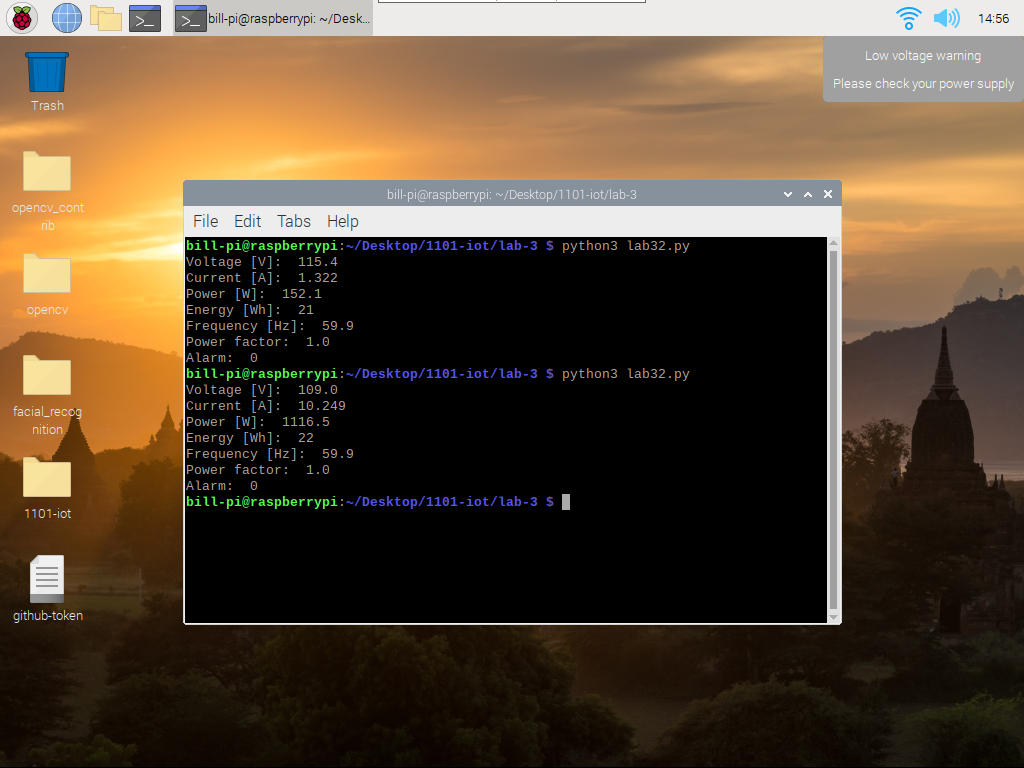
\includegraphics[width=0.6\textwidth]{img/1_res_hair_dryer_temp_file_1_then_2}
  \caption{Hair dryer result}
  \label{hair-dryer}
\end{figure}
\begin{figure}[h]
  \centering
  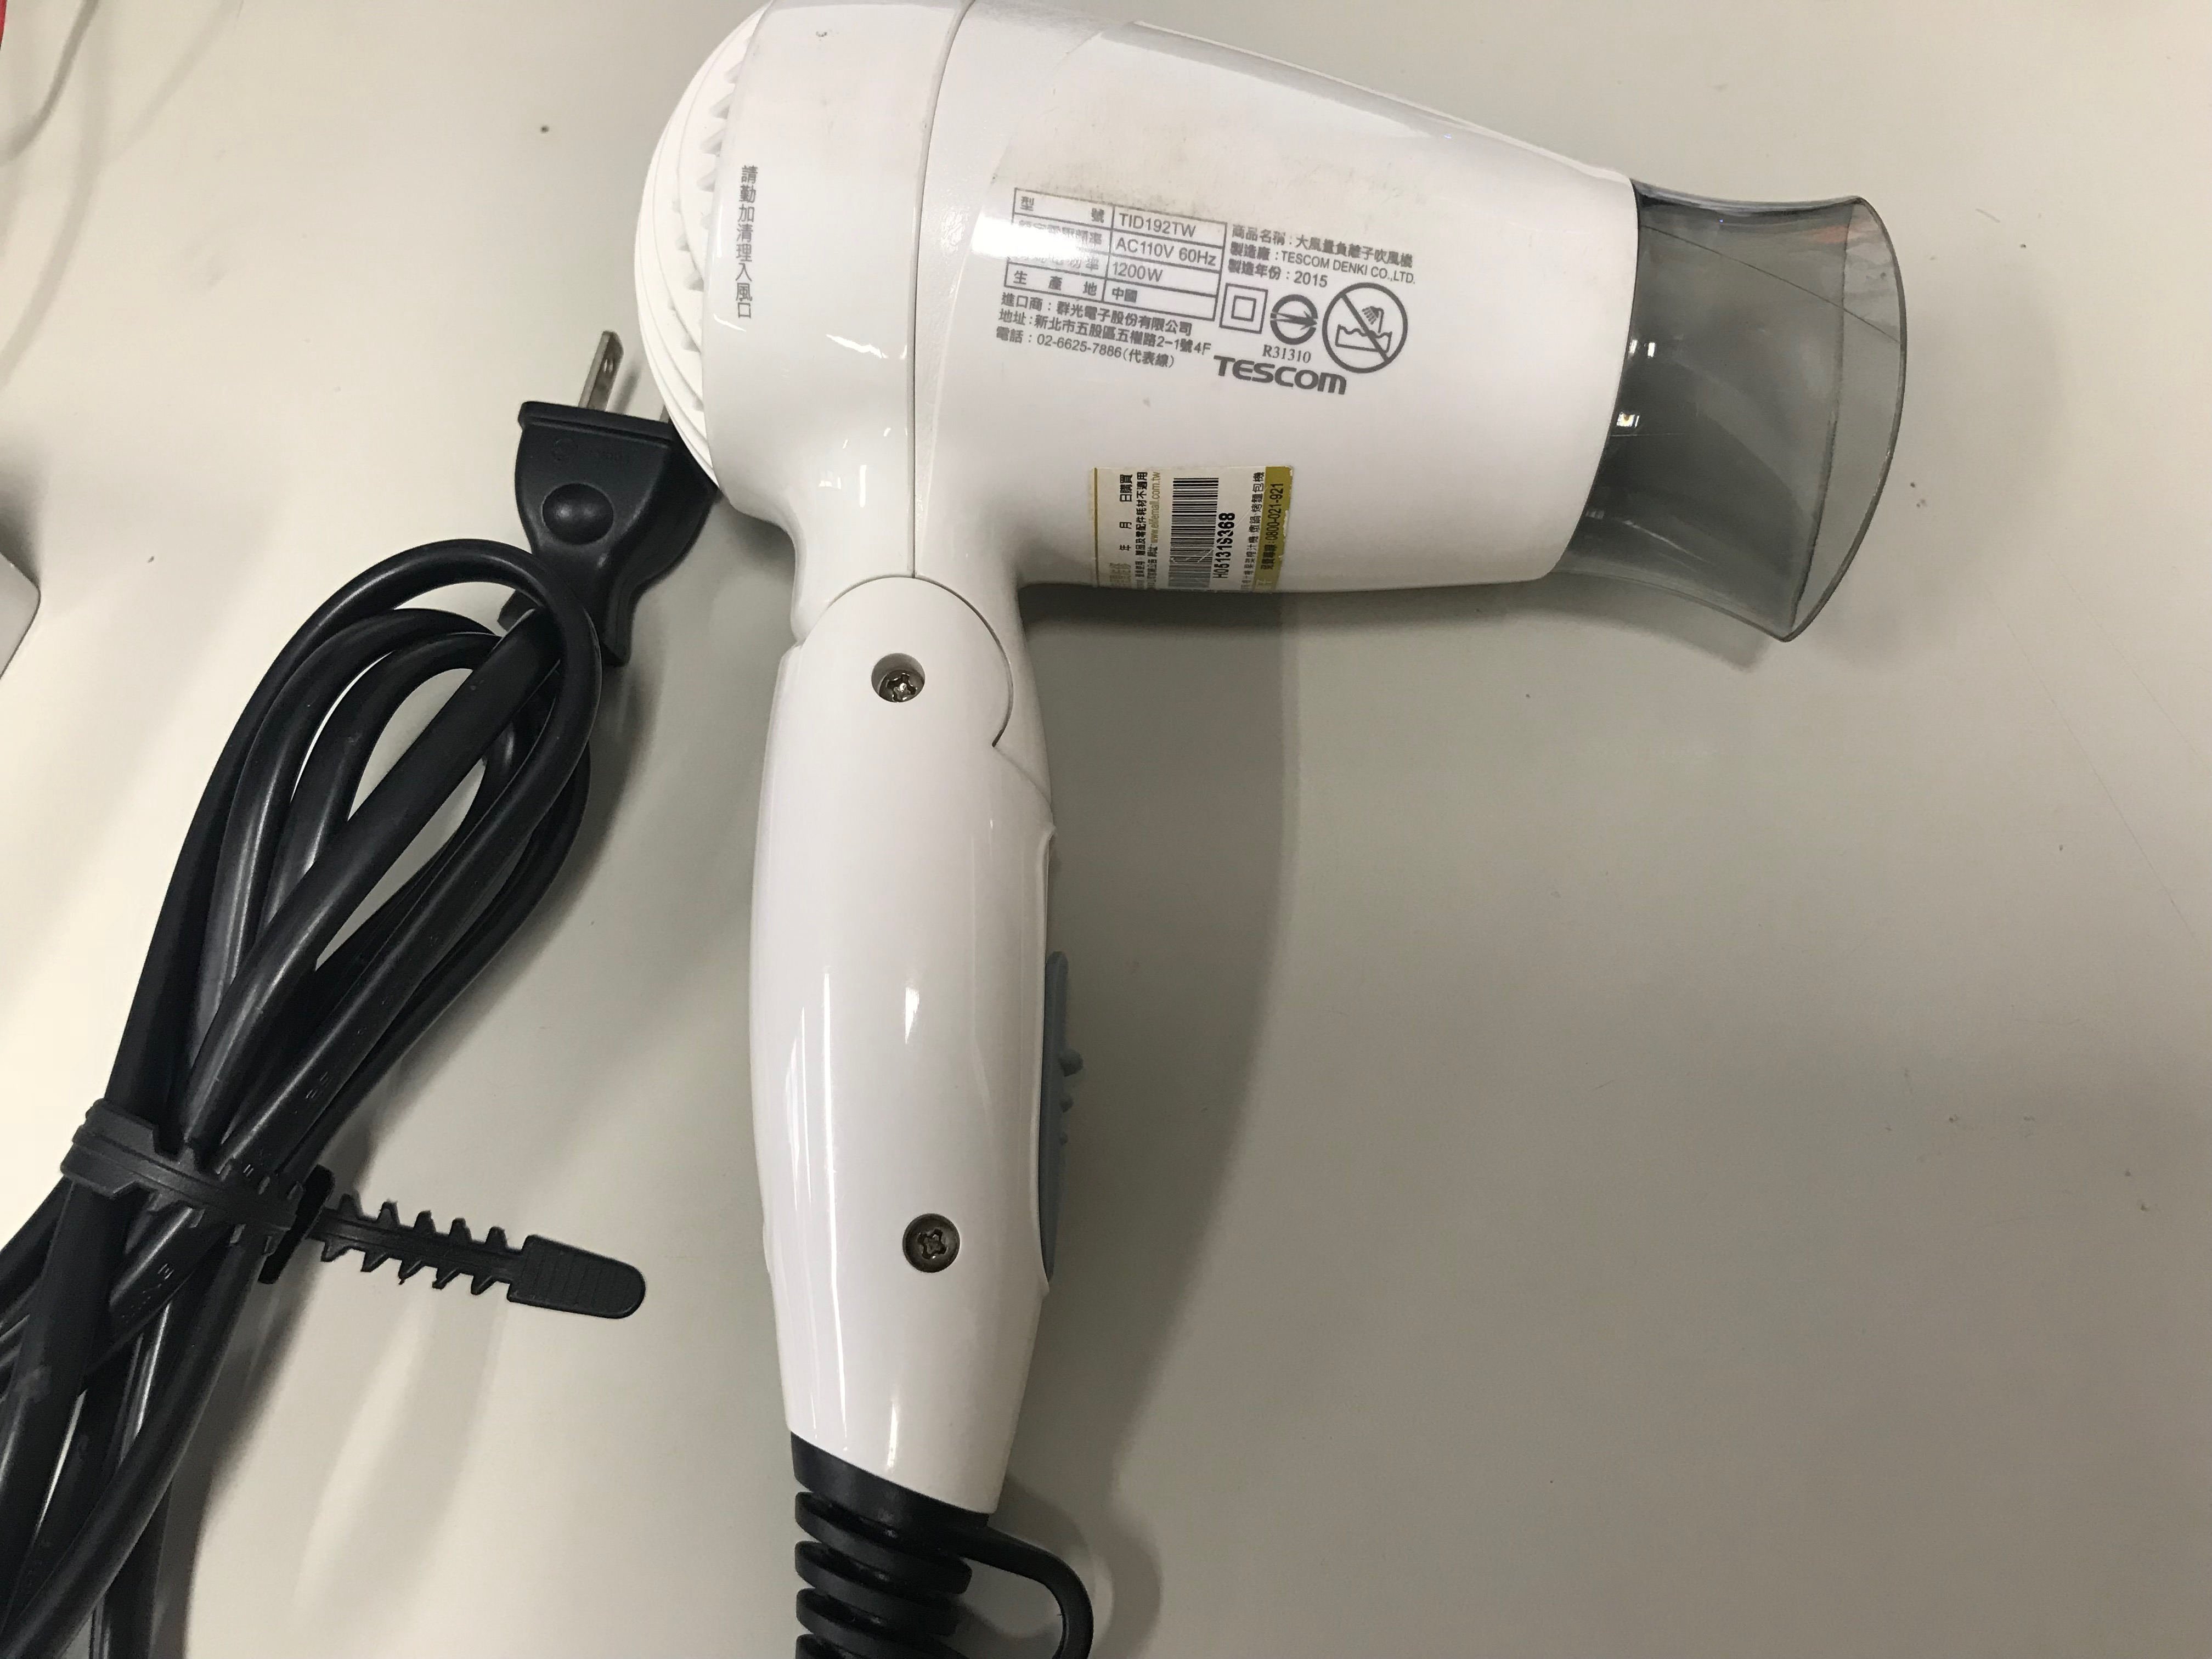
\includegraphics[width=0.6\textwidth]{img/1_spe_hair_dryer}
  \caption{Hair dryer specifications}
\end{figure}
\begin{figure}[h]
  \centering
  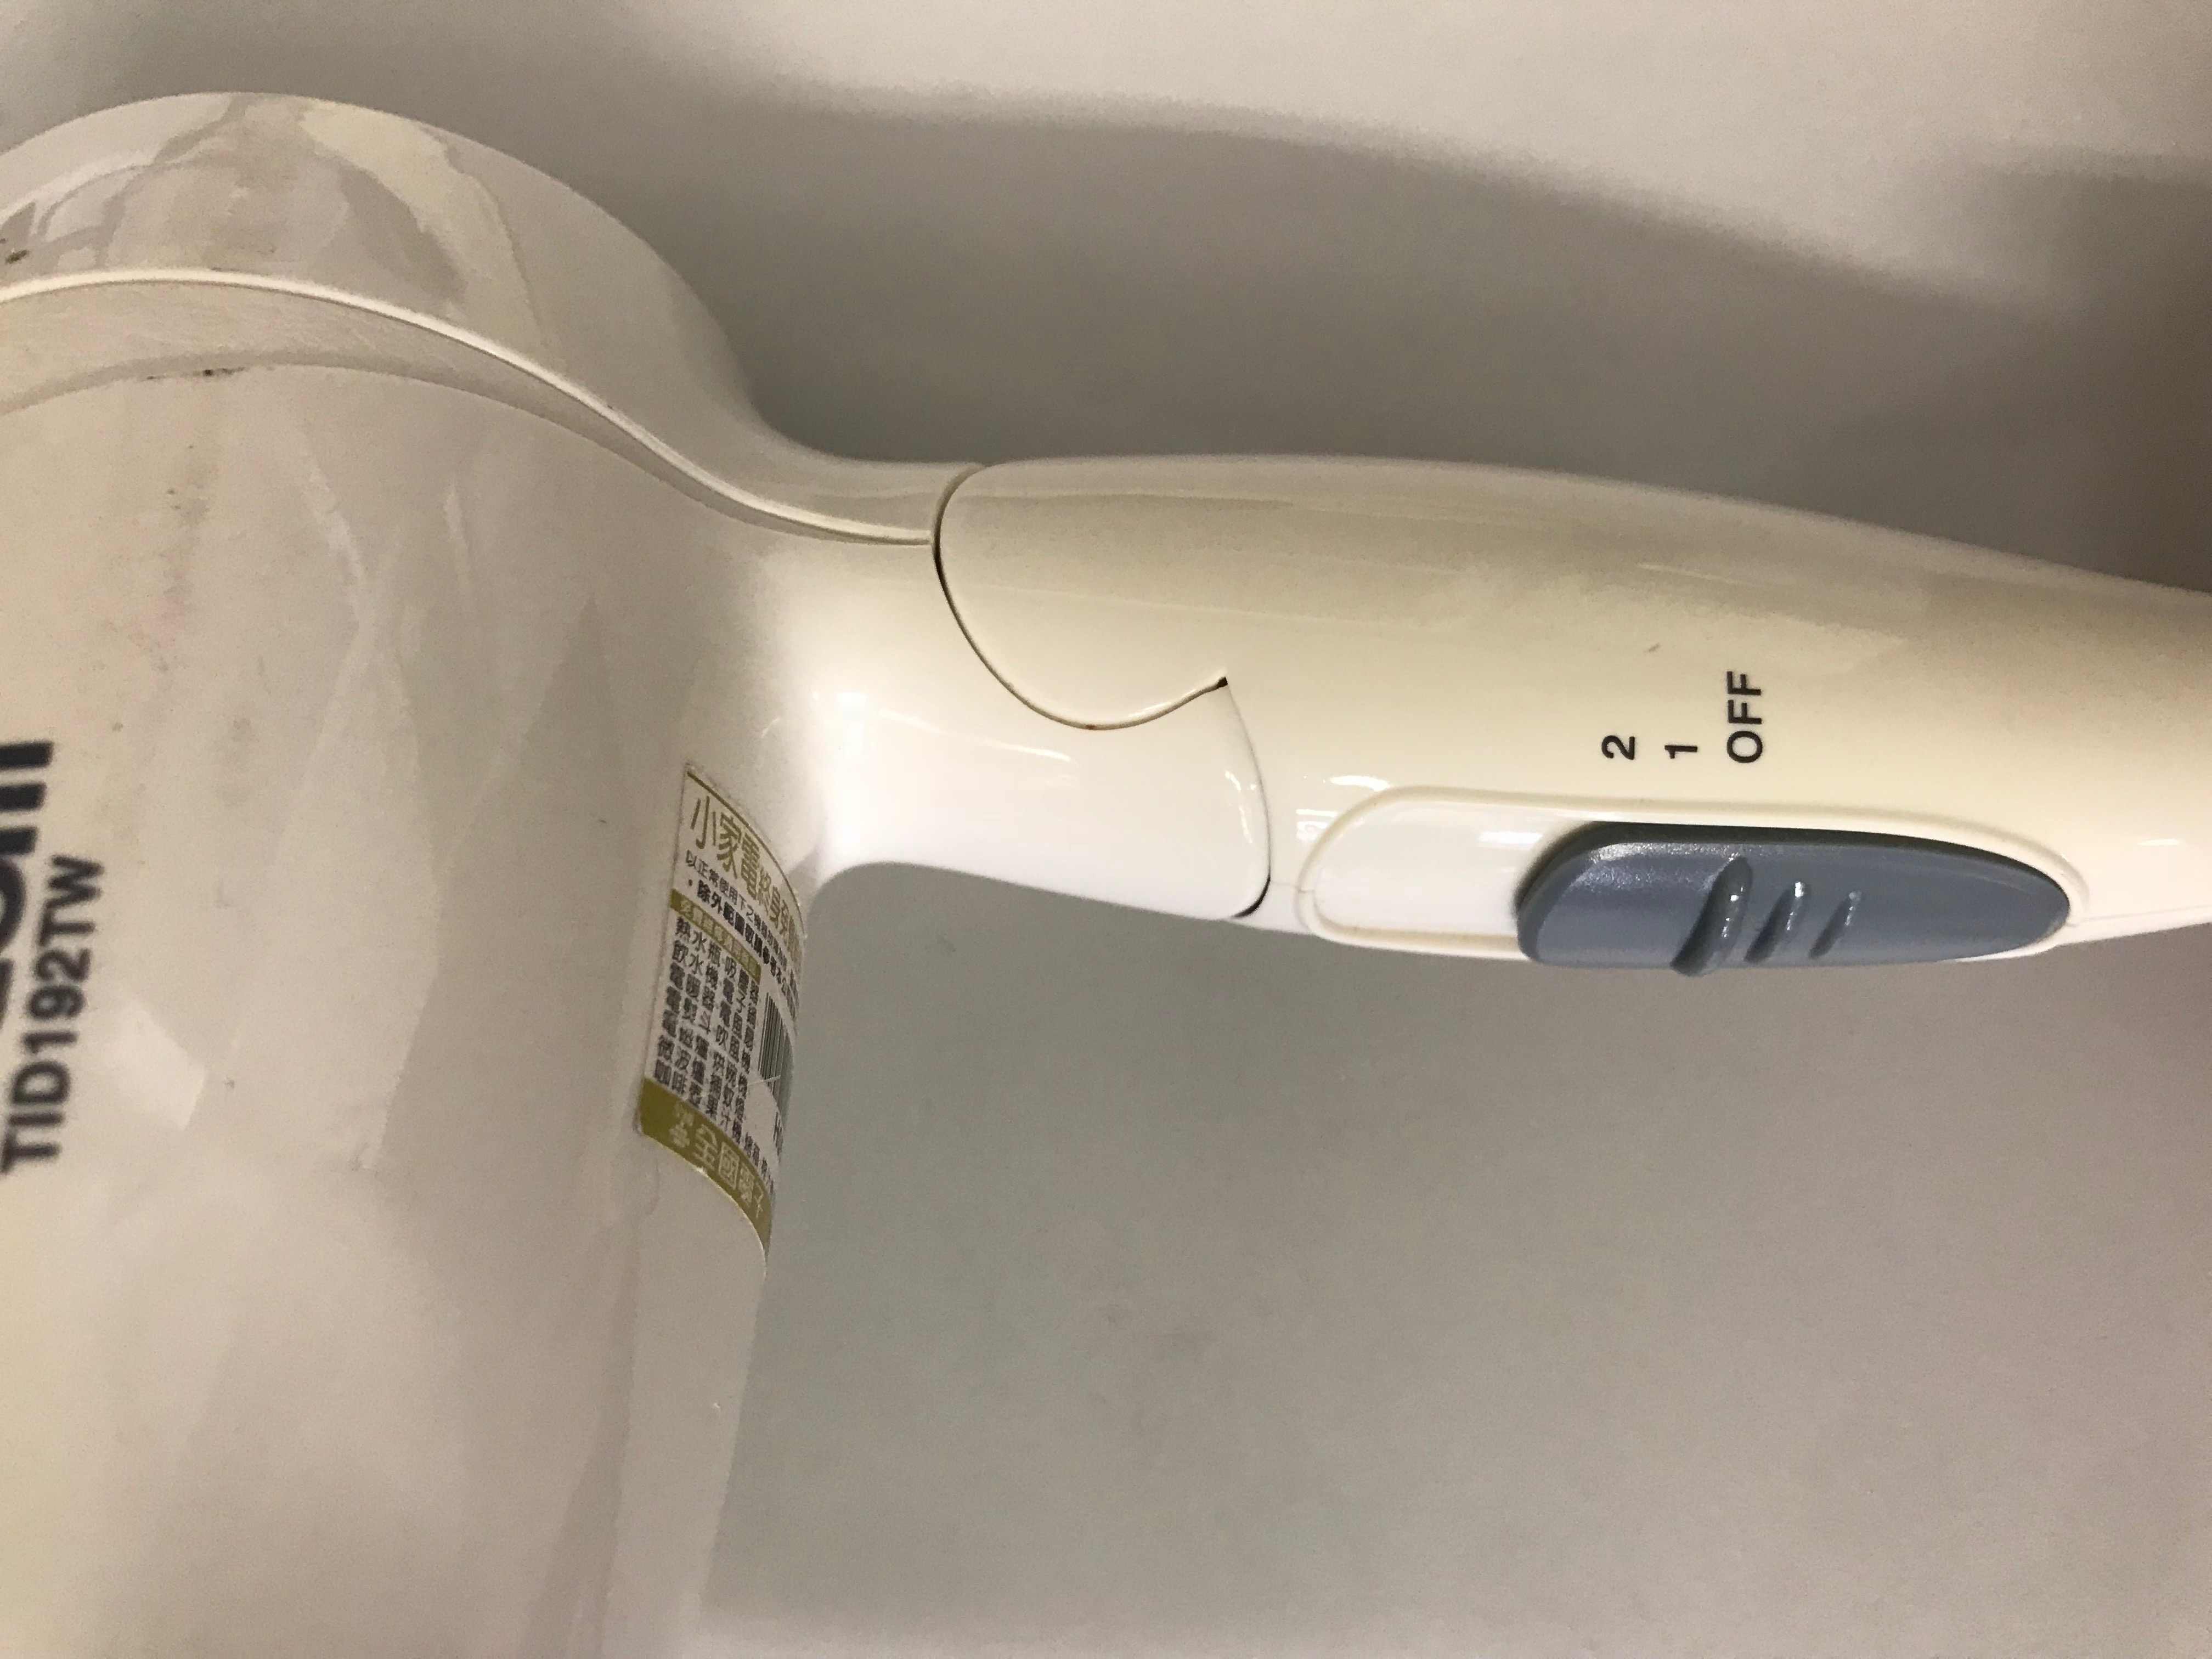
\includegraphics[angle=-90, origin=c, width=0.45\textwidth]{img/1_pic_hair_dryer_temp_file}
  \caption{Hair dryer temperature files}
\end{figure}

\clearpage

\subsection{Electric fan}
The process is pretty much the same for the electric fan: We first switch the speed button level to the lowest, recording the measurements, and then move on to the highest speed. Figure \ref{electric-fan} illustrates a two-third power ratio in the former test relative to the latter one, which corresponds to their respective fan speeds.
\begin{figure}[h]
  \centering
  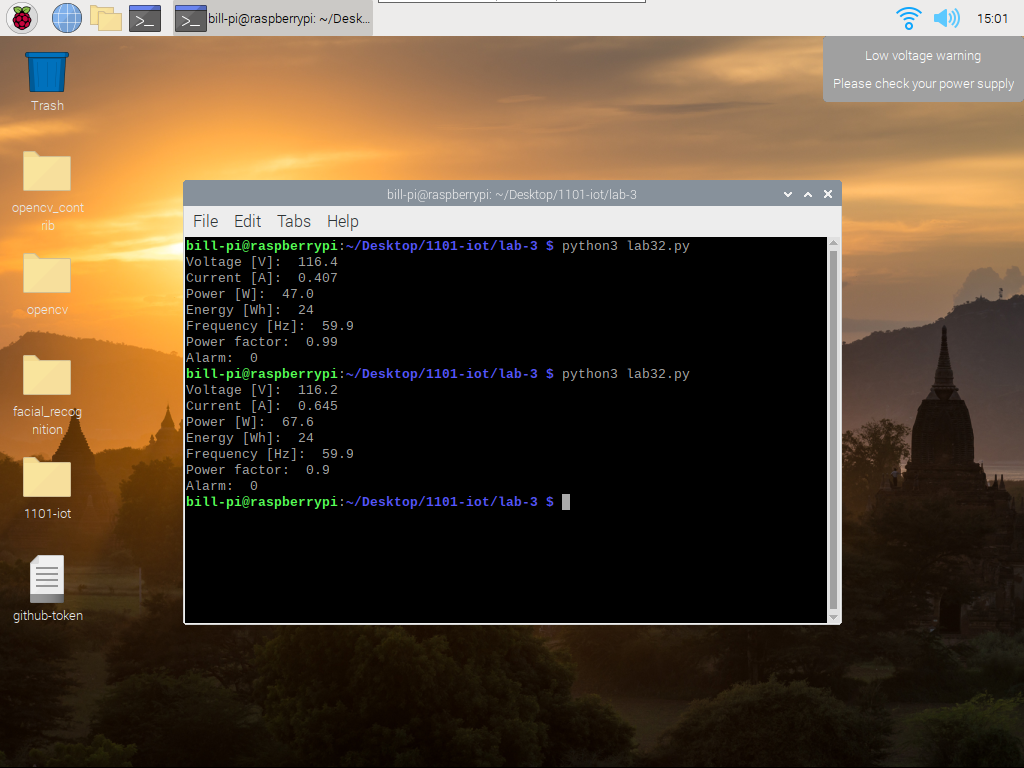
\includegraphics[width=0.6\textwidth]{img/2_res_electric_fan_speed_button_low_then_high}
  \caption{Electric fan result}
  \label{electric-fan}
\end{figure}
\begin{figure}[h]
  \centering
  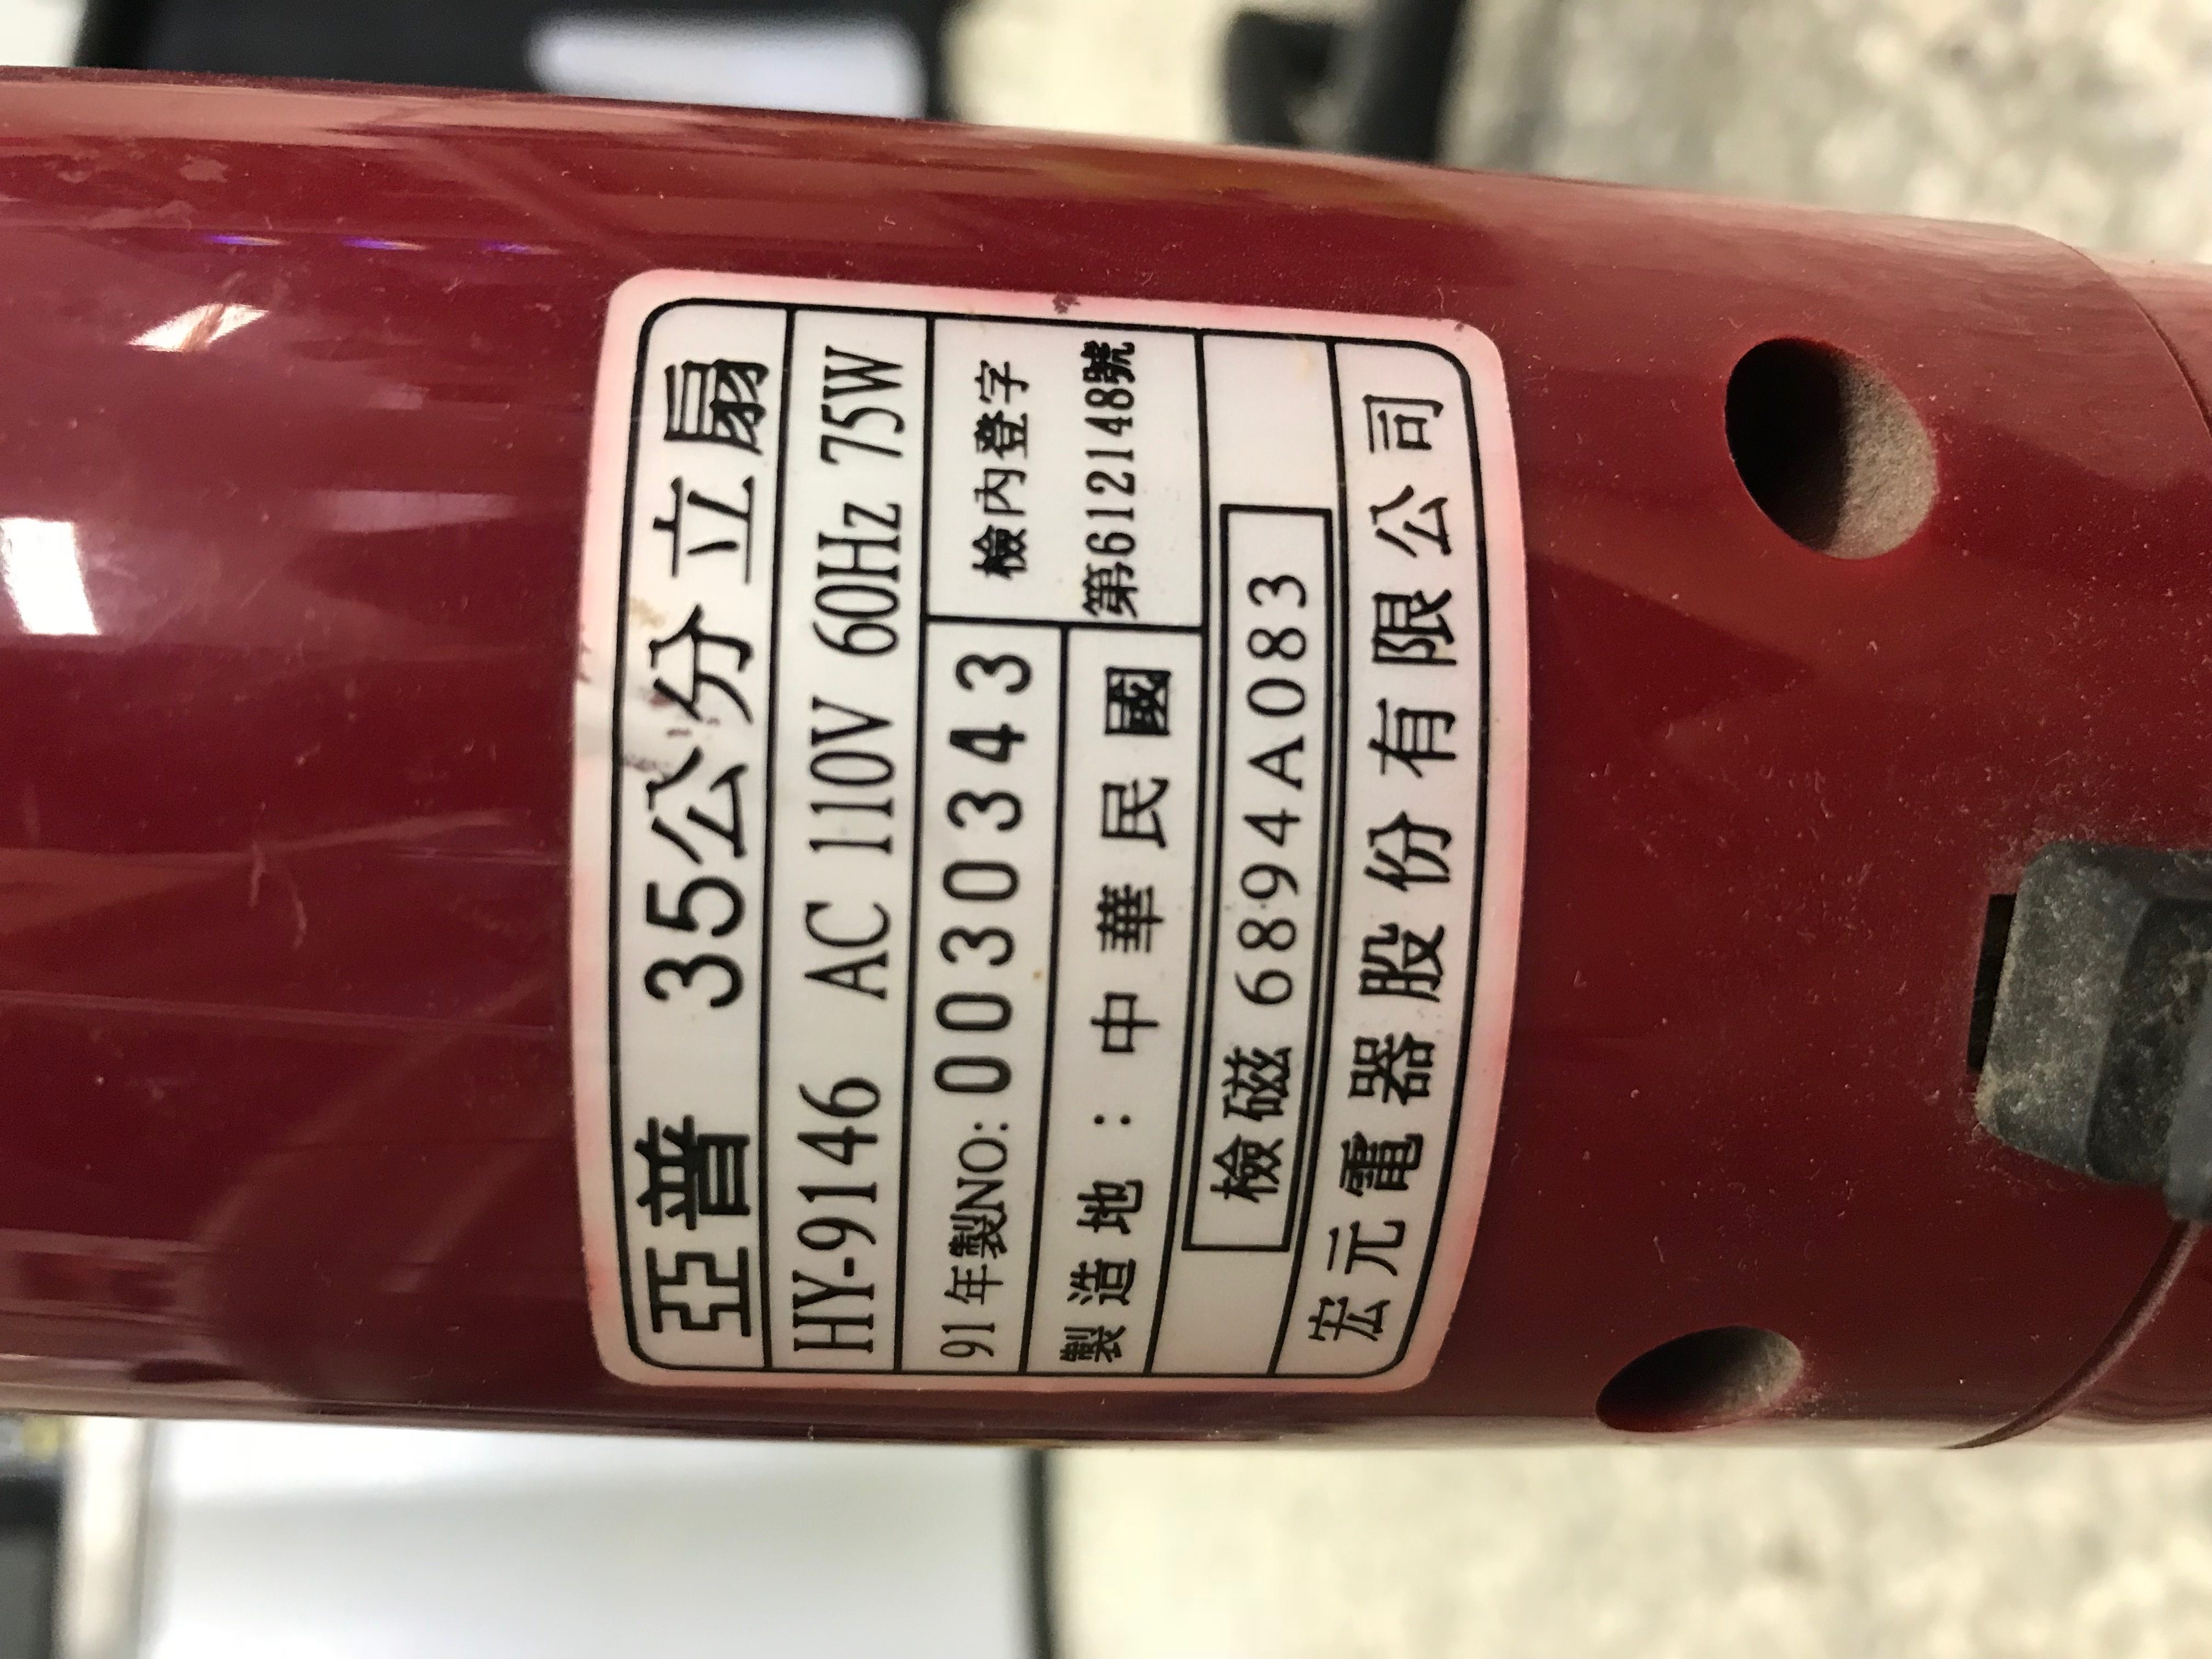
\includegraphics[angle=-90, origin=c, width=0.45\textwidth]{img/2_spe_electric_fan}
  \caption{Electric fan specifications}
\end{figure}
\begin{figure}[h]
  \centering
  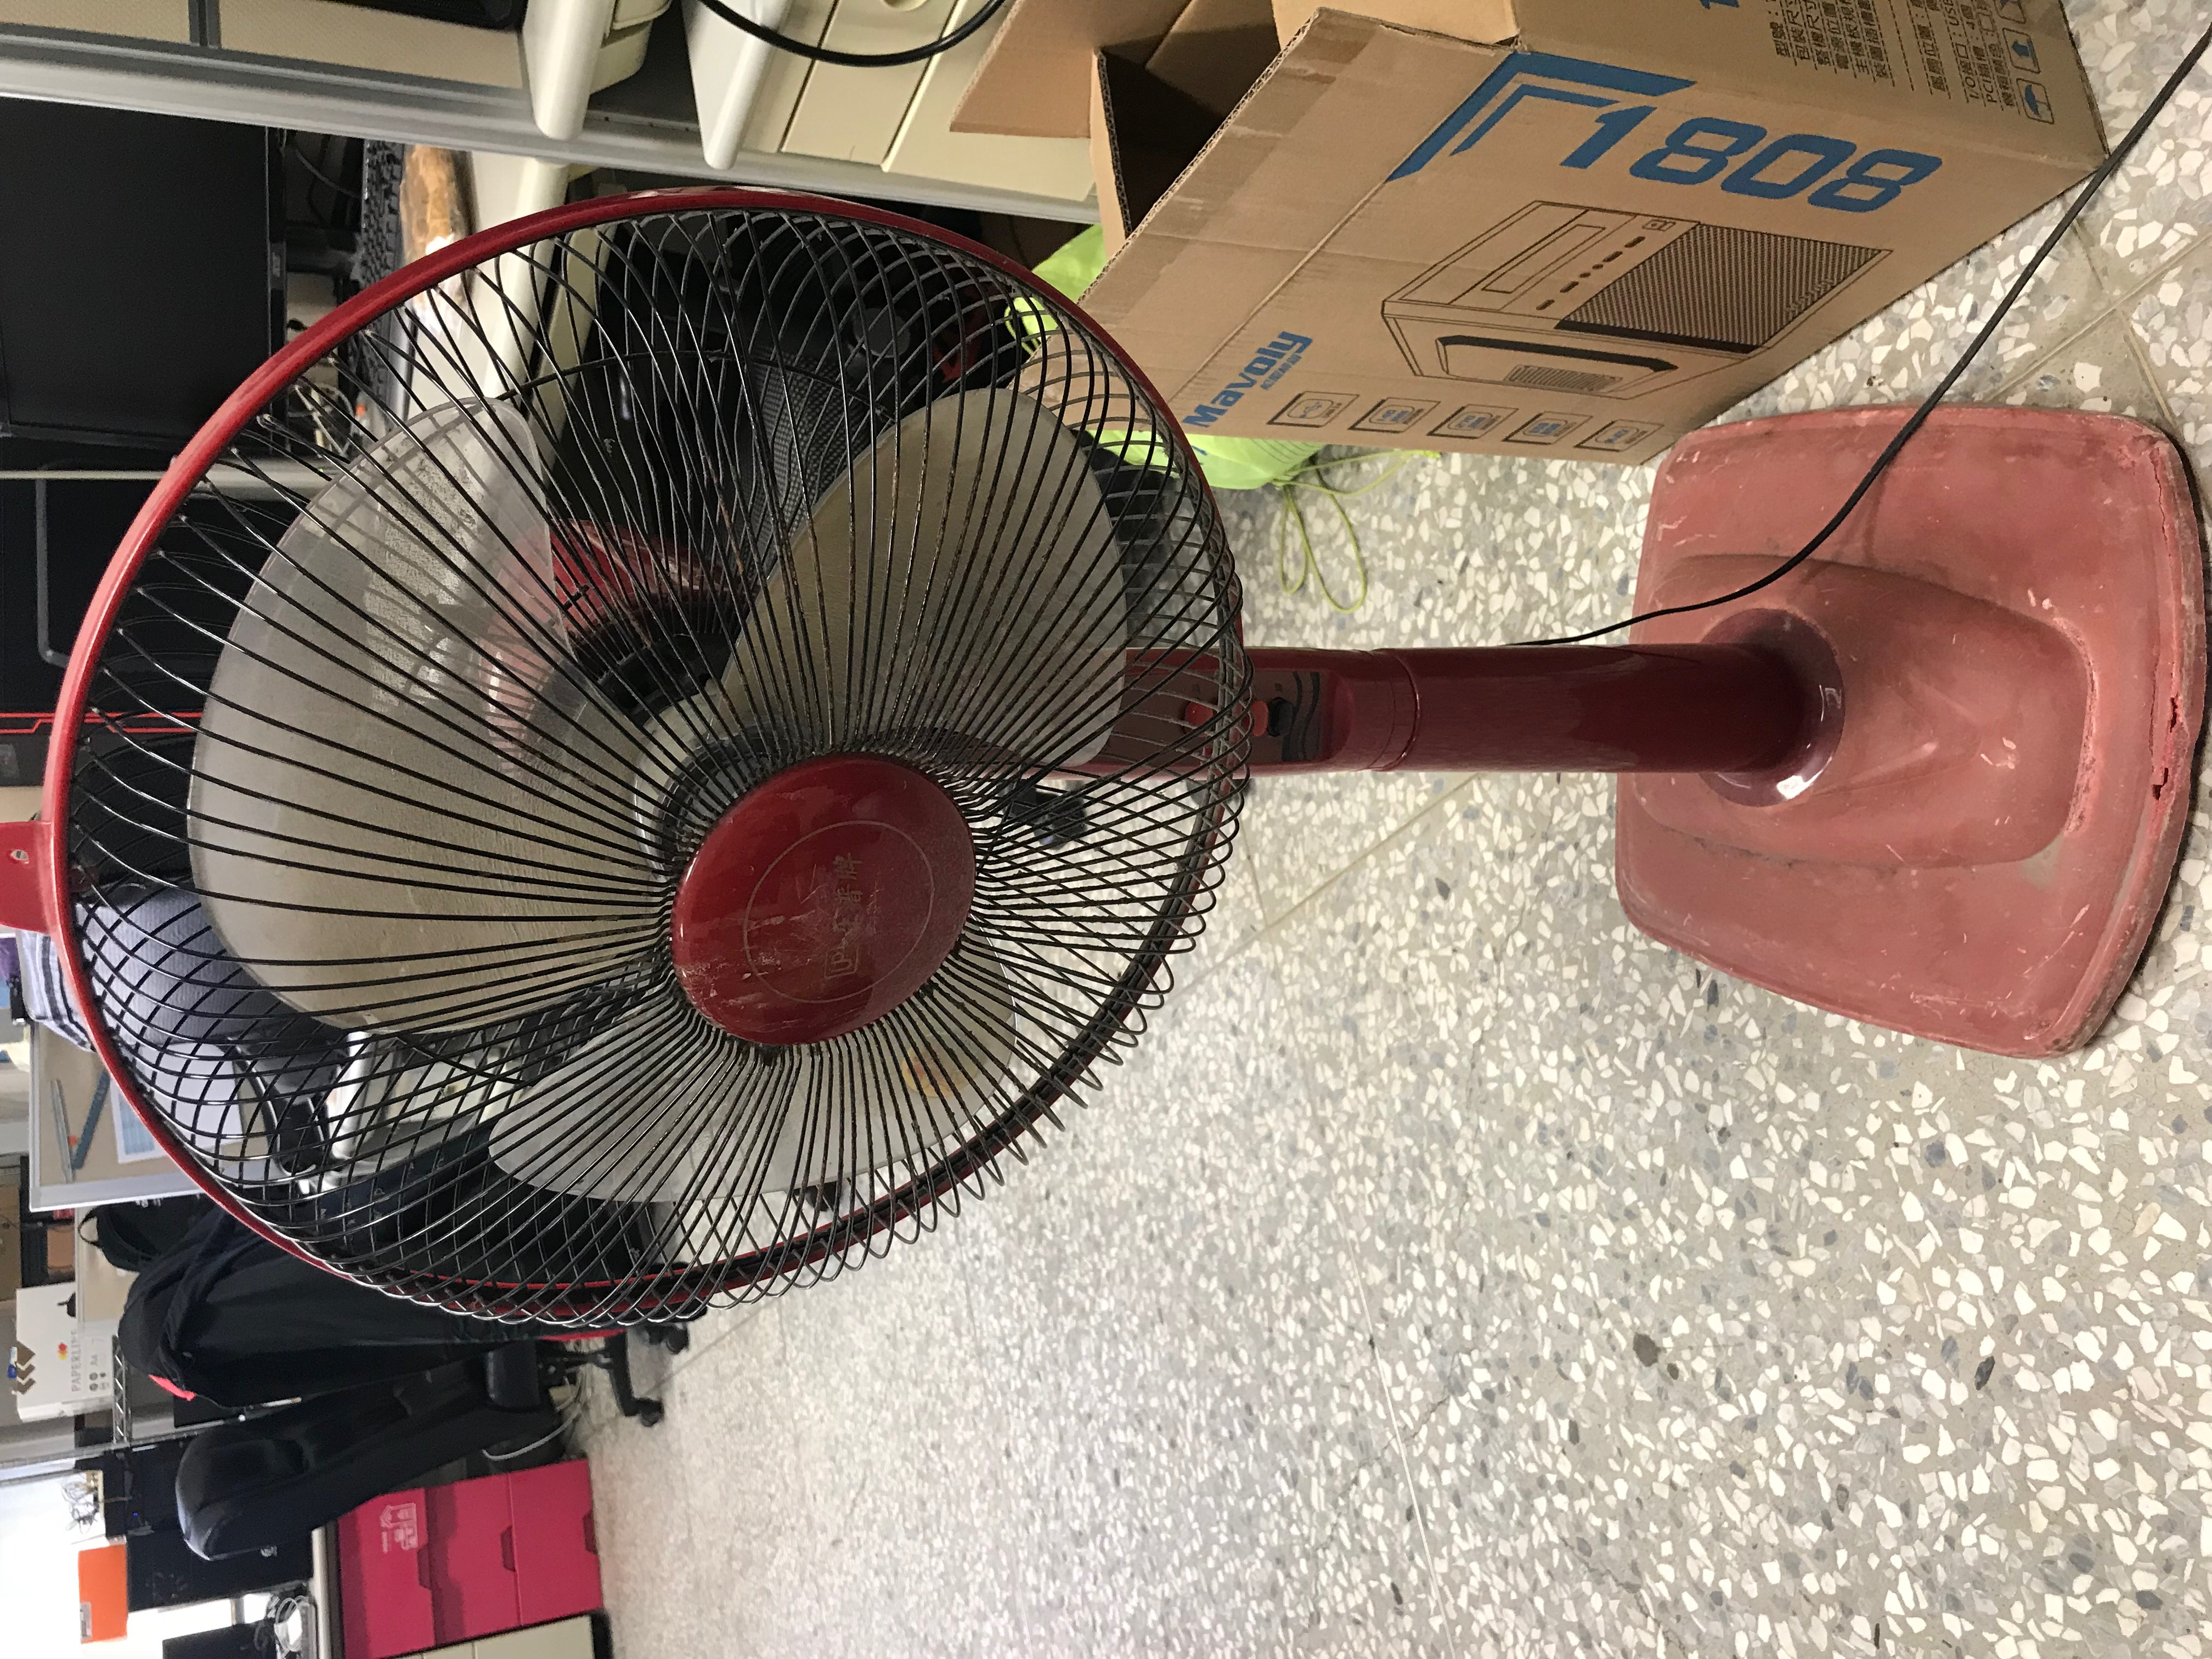
\includegraphics[angle=-90, origin=c, width=0.45\textwidth]{img/2_pic_elecric_fan}
  \caption{Electric fan}
\end{figure}
\begin{figure}[h]
  \centering
  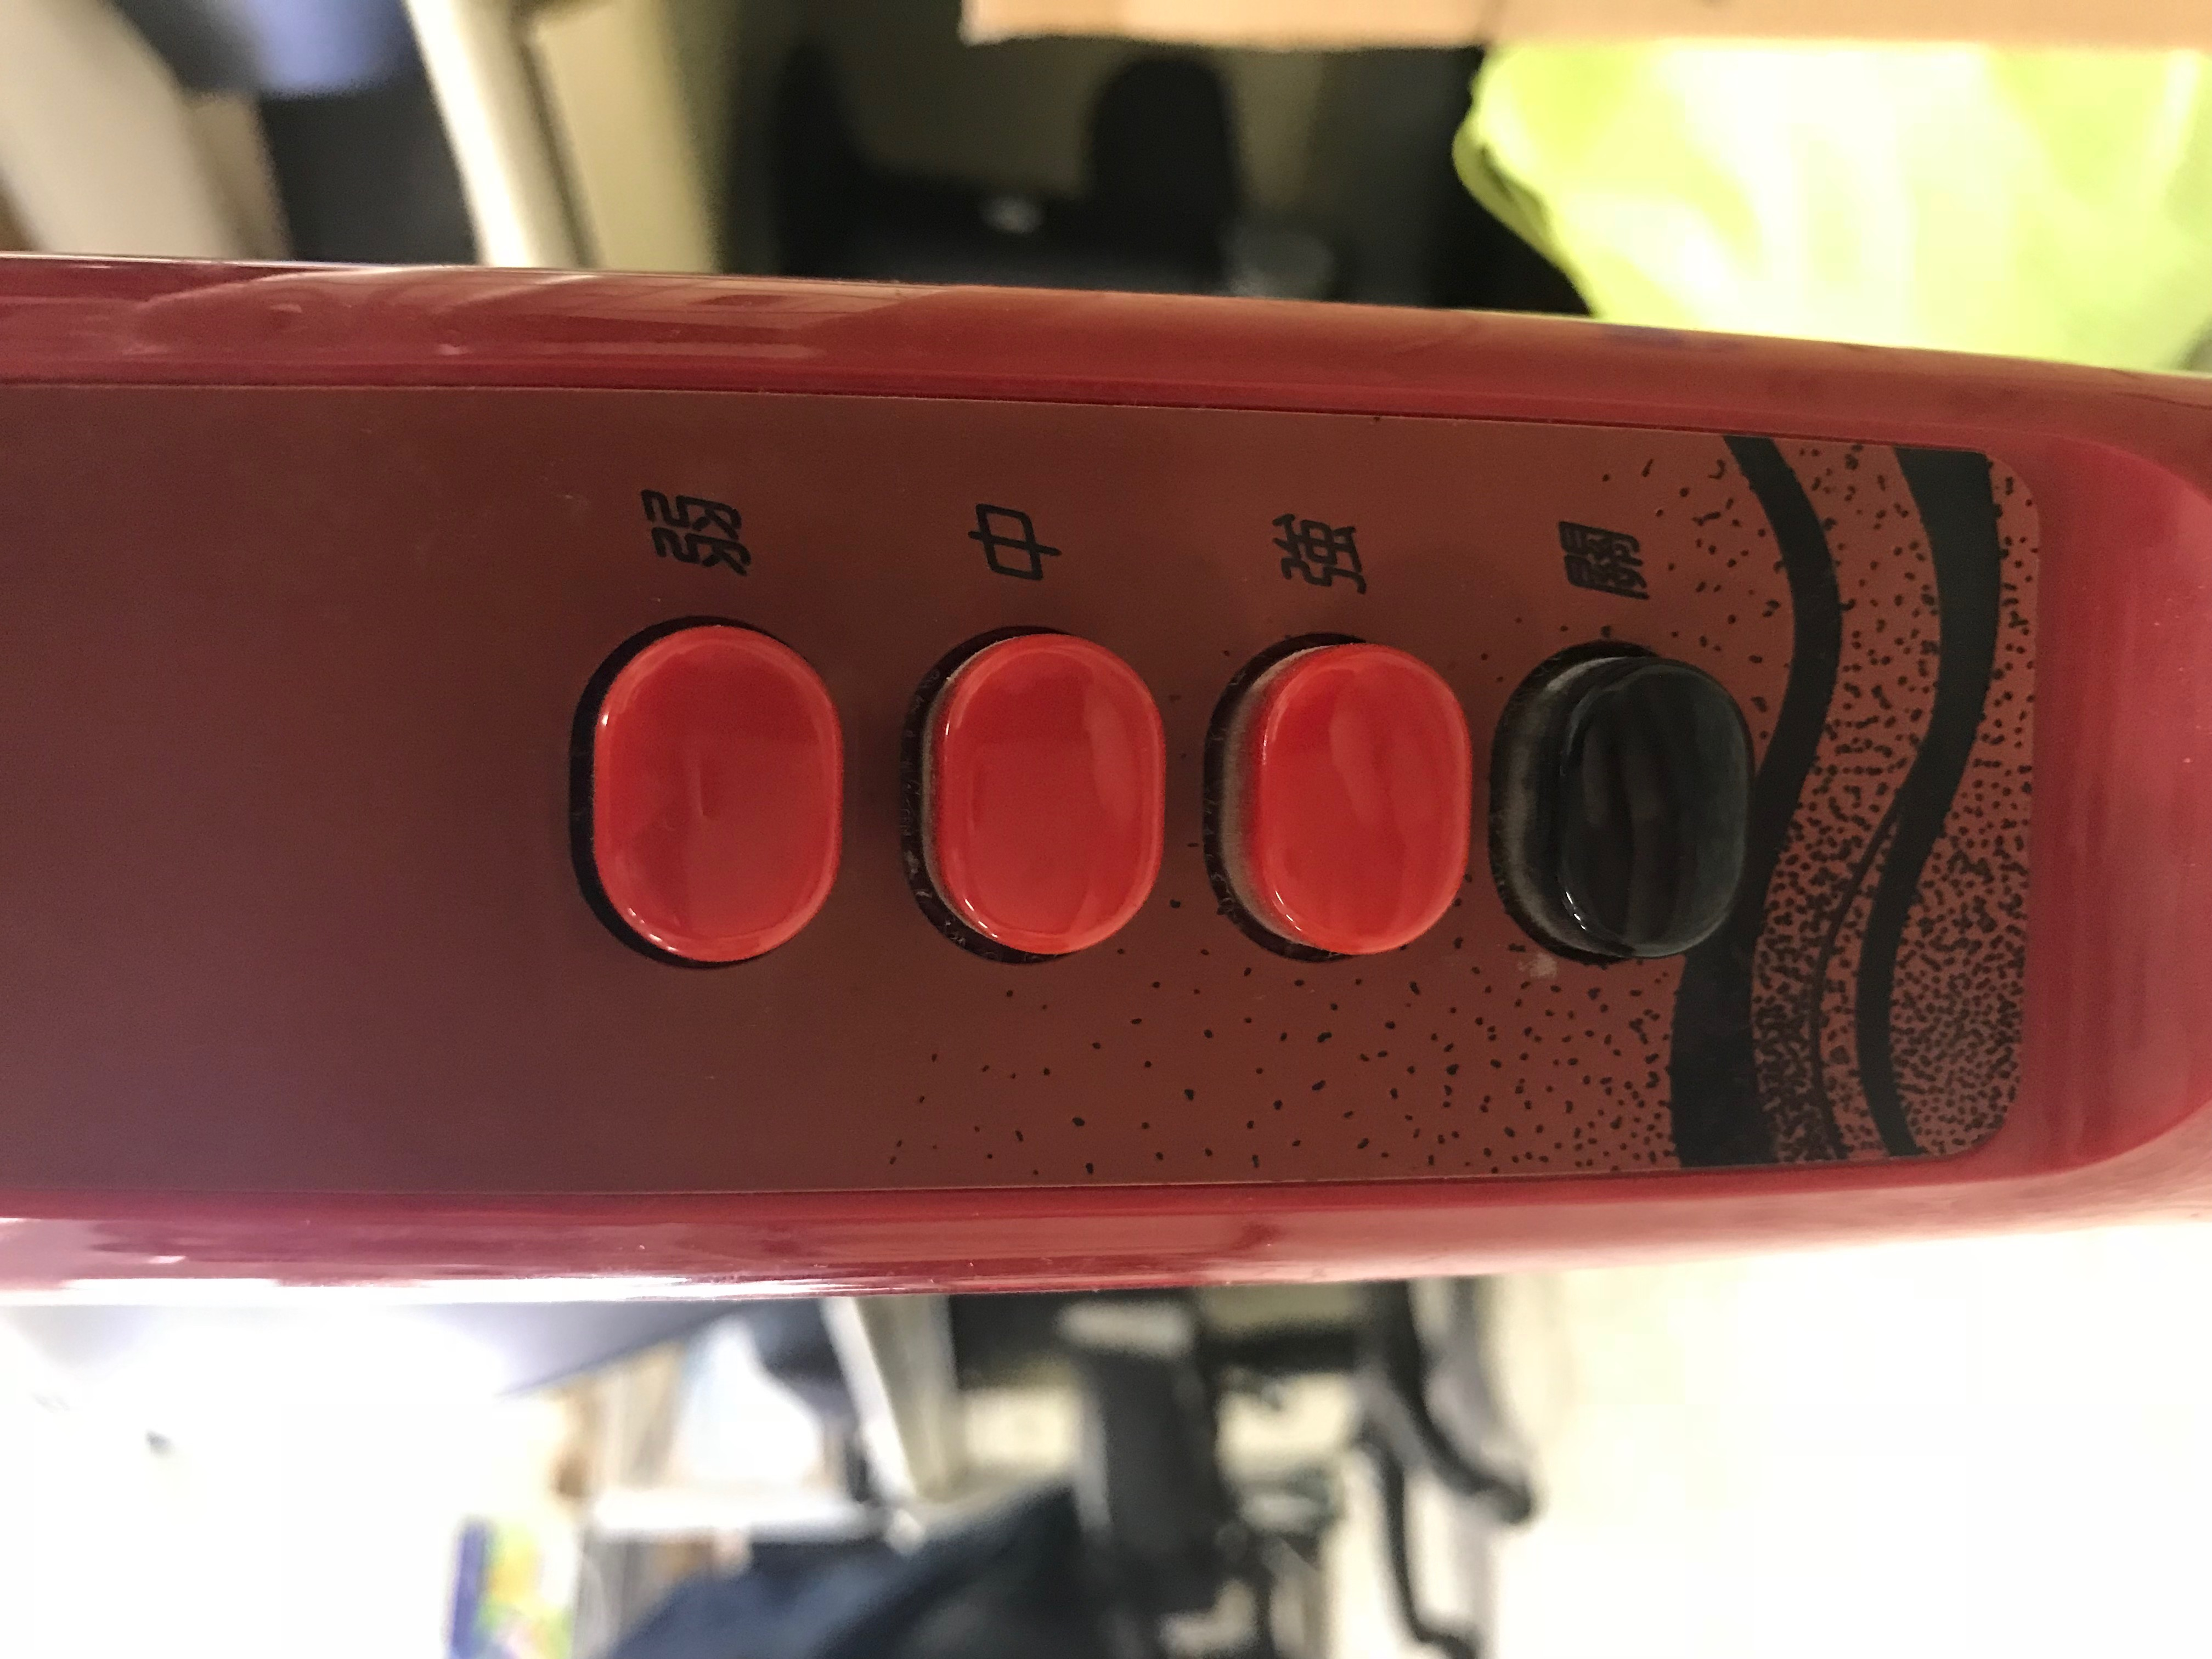
\includegraphics[angle=-90, origin=c, width=0.45\textwidth]{img/2_pic_electric_fan_speed_button}
  \caption{Electric fan speed buttons}
\end{figure}

\clearpage

\subsection{Table lamp}
Subsequent tests are comparatively straightforward: We plug in the power cable, turning on the device, and then record the data. The results are depicted in the several figures.
\begin{figure}[h]
  \centering
  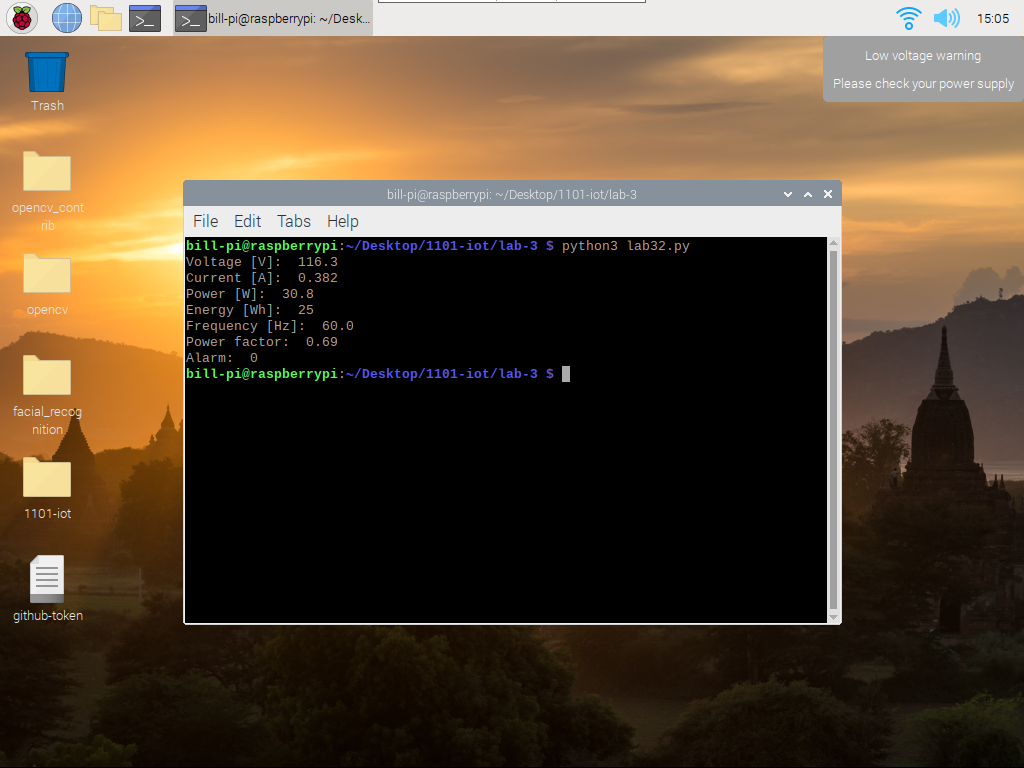
\includegraphics[width=0.6\textwidth]{img/3_res_table_lamp}
  \caption{Table lamp result}
\end{figure}
\begin{figure}[h]
  \centering
  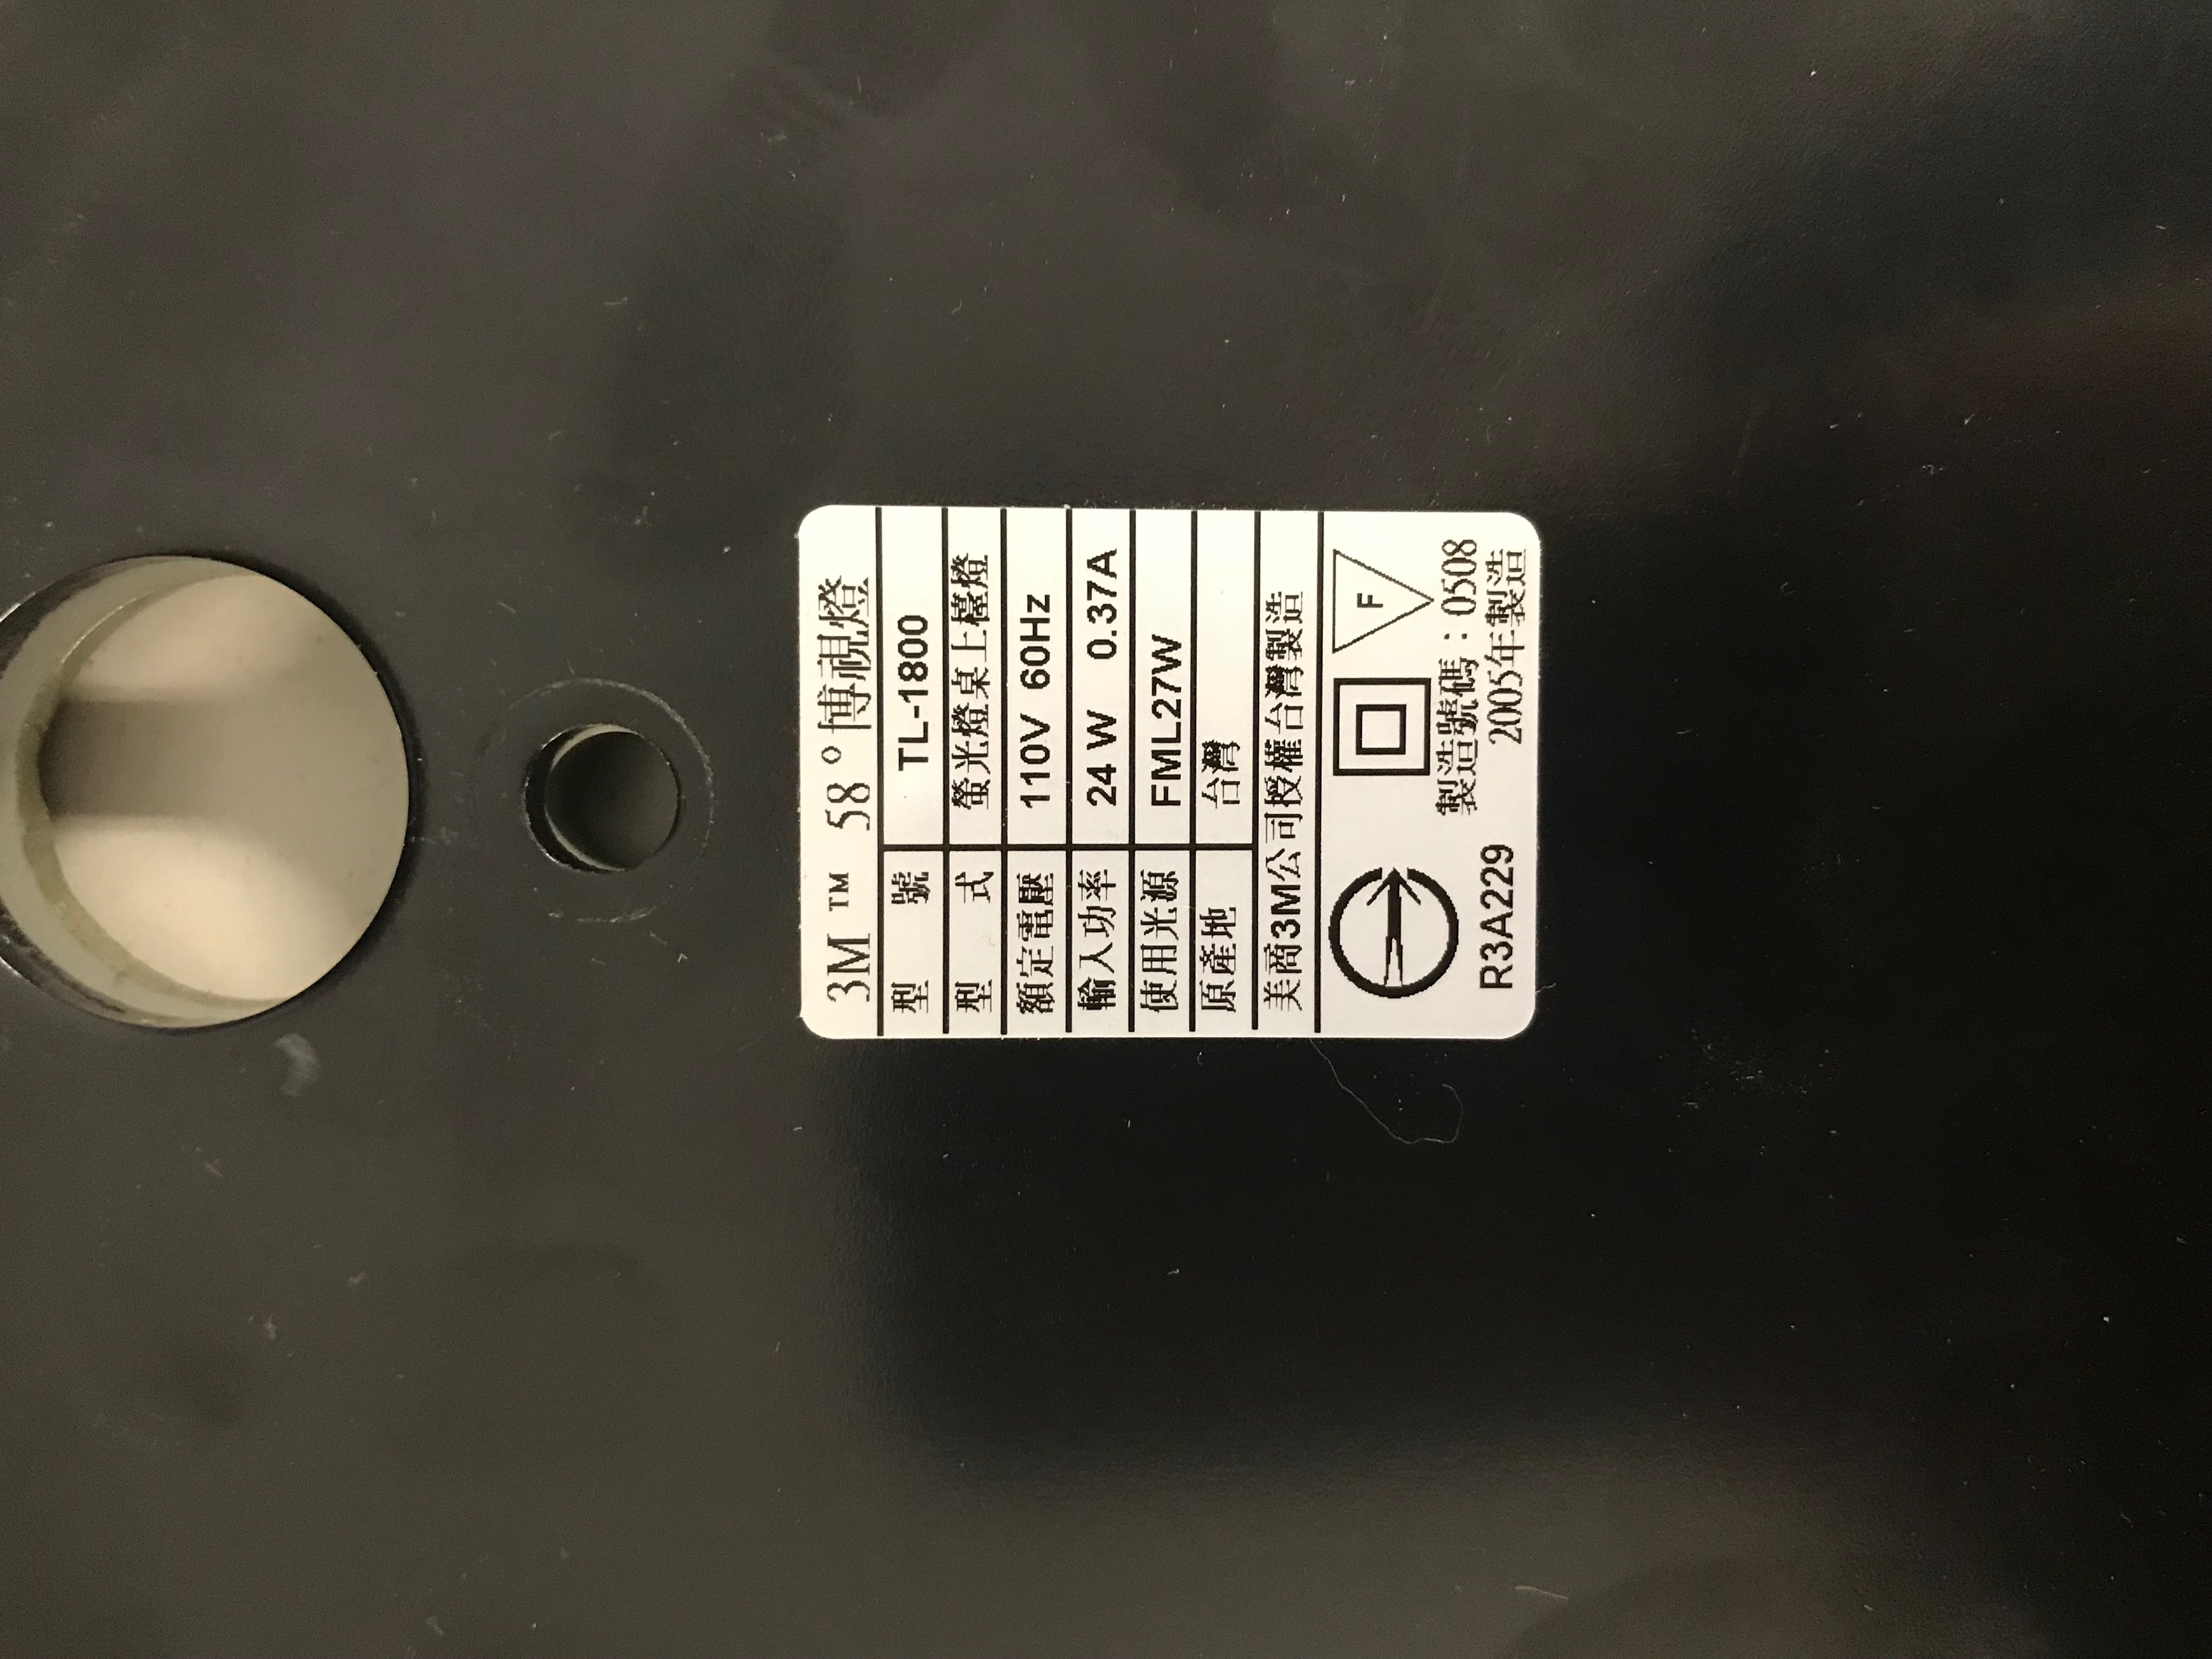
\includegraphics[angle=-90, origin=c, width=0.45\textwidth]{img/3_spe_table_lamp}
  \caption{Table lamp specifications}
\end{figure}
\begin{figure}[h]
  \centering
  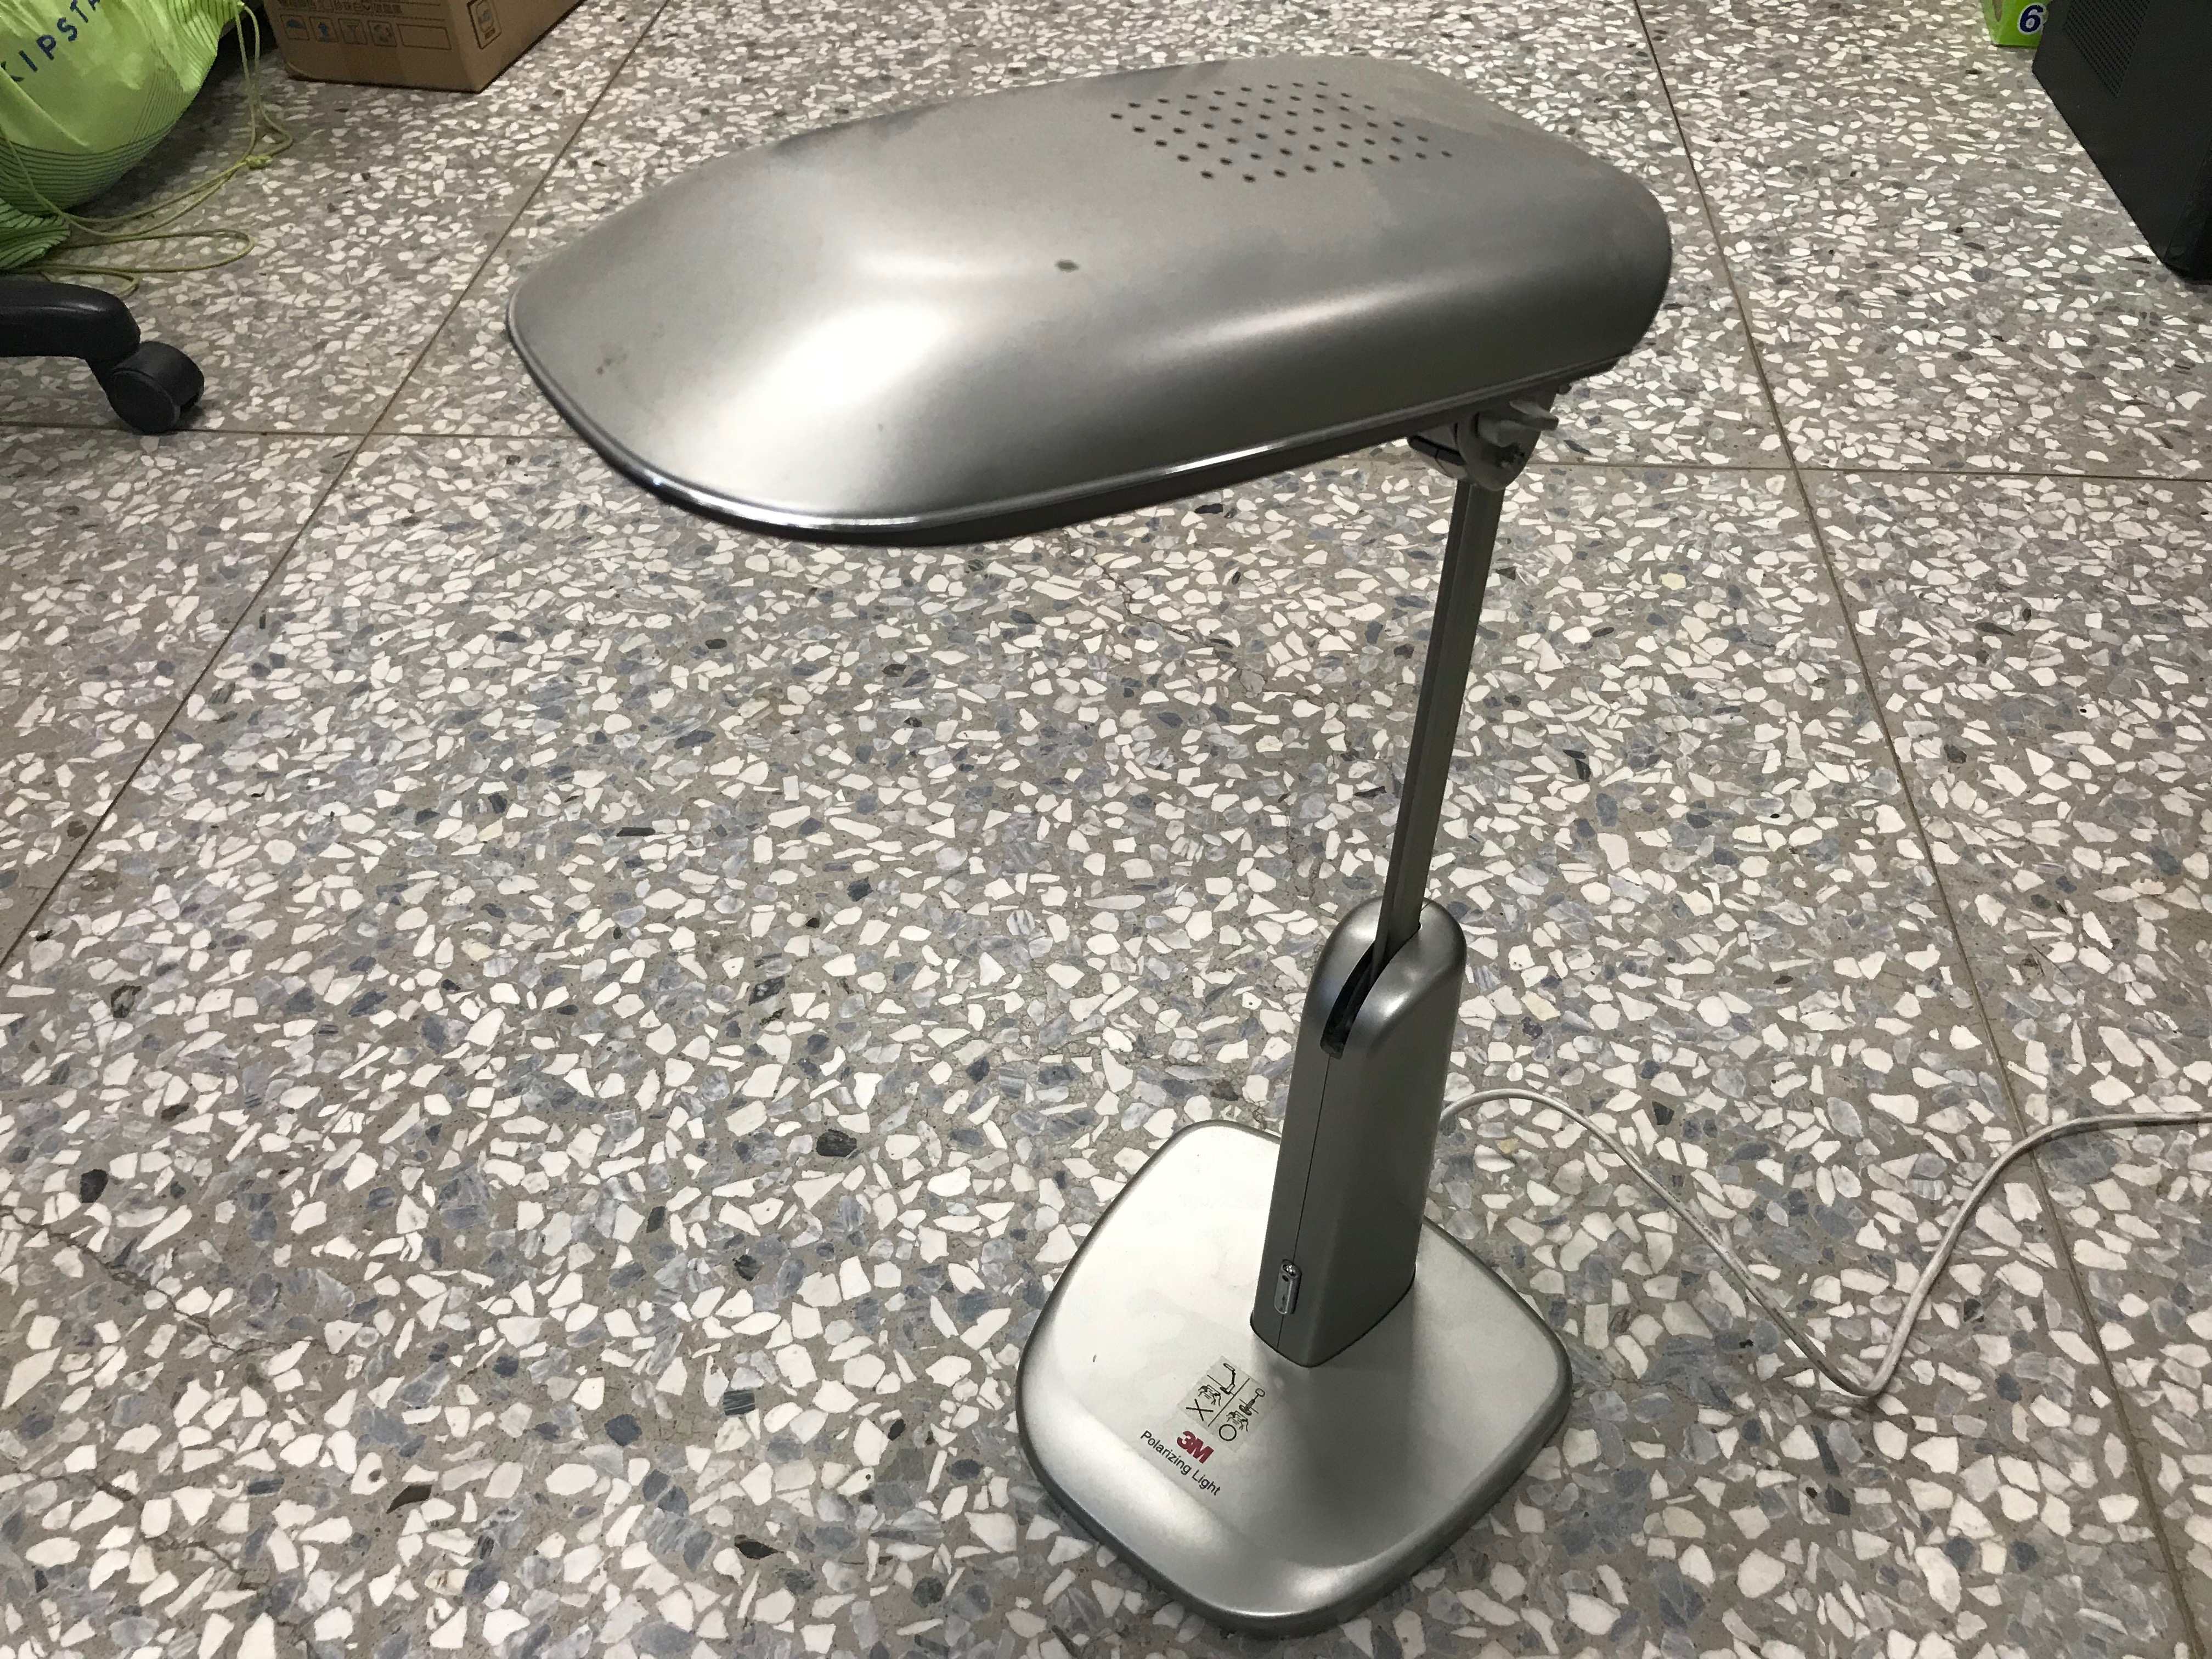
\includegraphics[width=0.6\textwidth]{img/3_pic_table_lamp}
  \caption{Table lamp}
\end{figure}

\clearpage

\subsection{Speaker}
\begin{figure}[h]
  \centering
  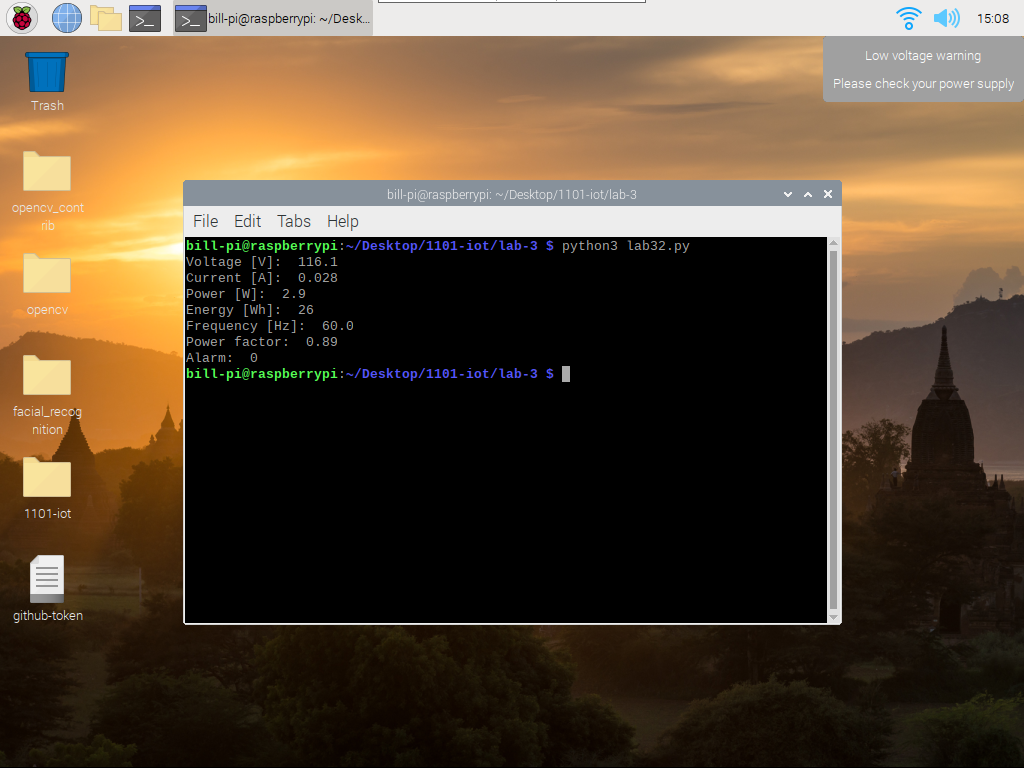
\includegraphics[width=0.6\textwidth]{img/4_res_speaker}
  \caption{Speaker result}
\end{figure}
\begin{figure}[h]
  \centering
  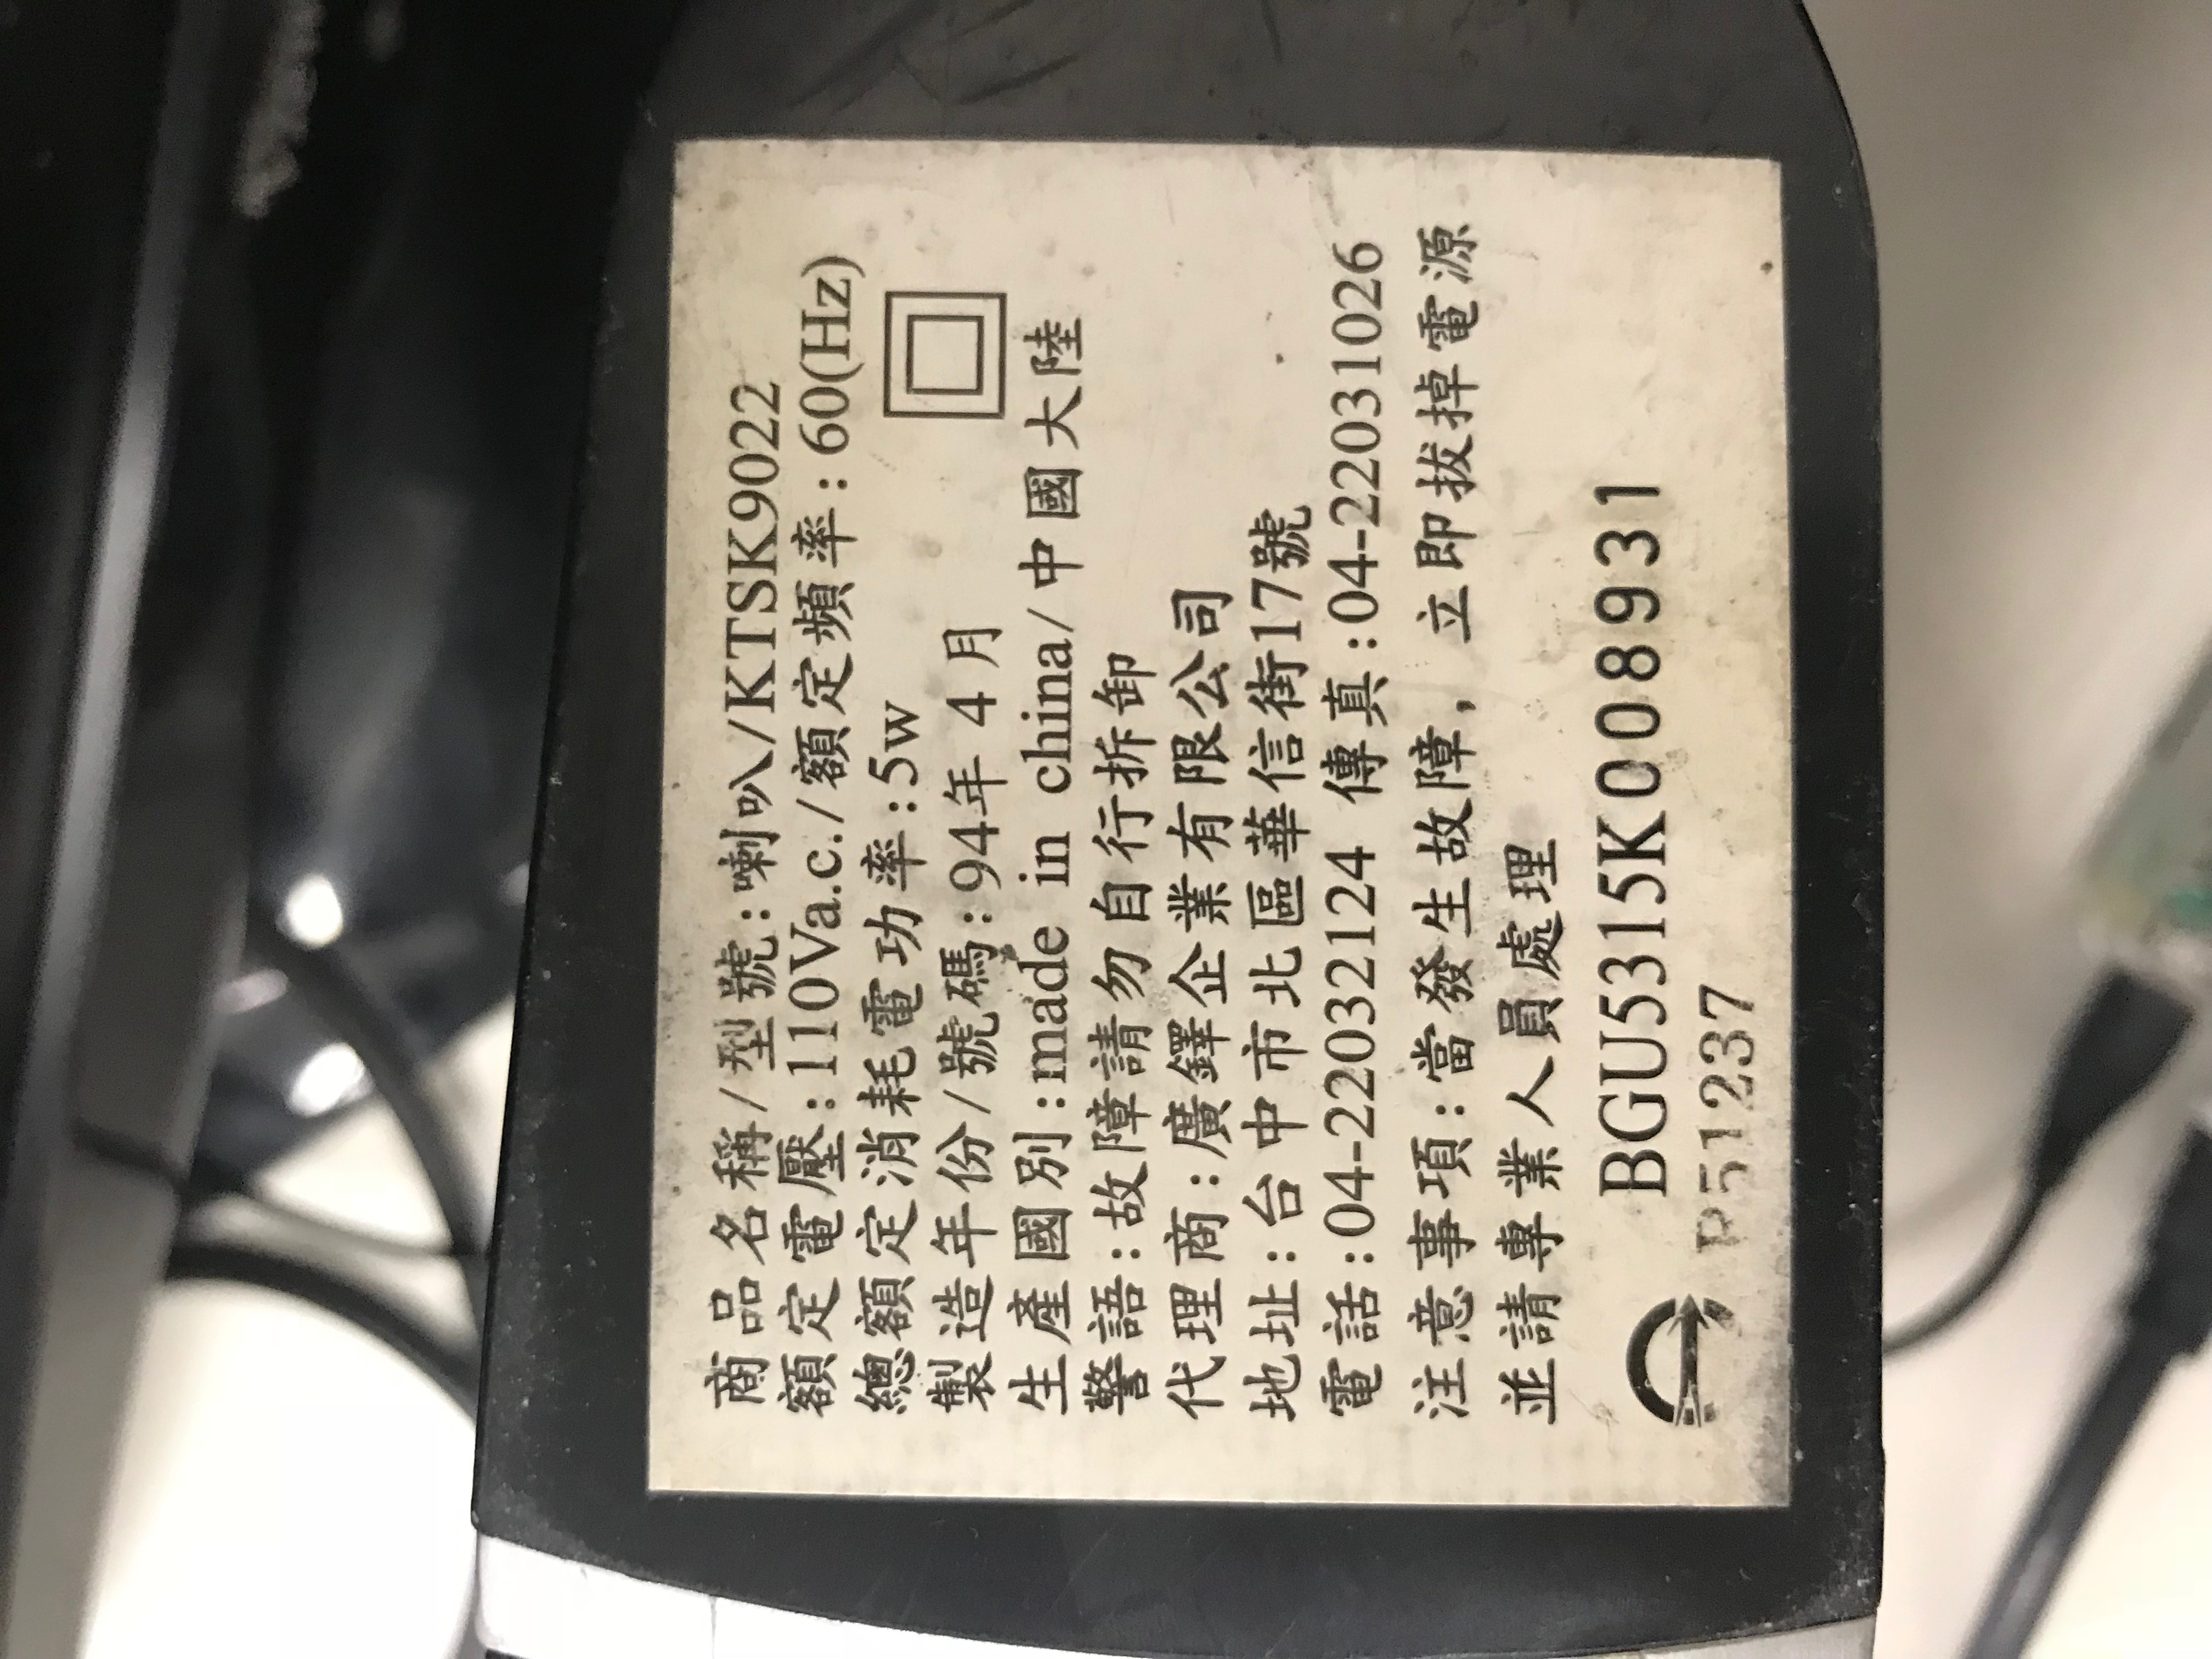
\includegraphics[angle=-90, origin=c, width=0.45\textwidth]{img/4_spe_speaker}
  \caption{Speaker specifications}
\end{figure}
\begin{figure}[h]
  \centering
  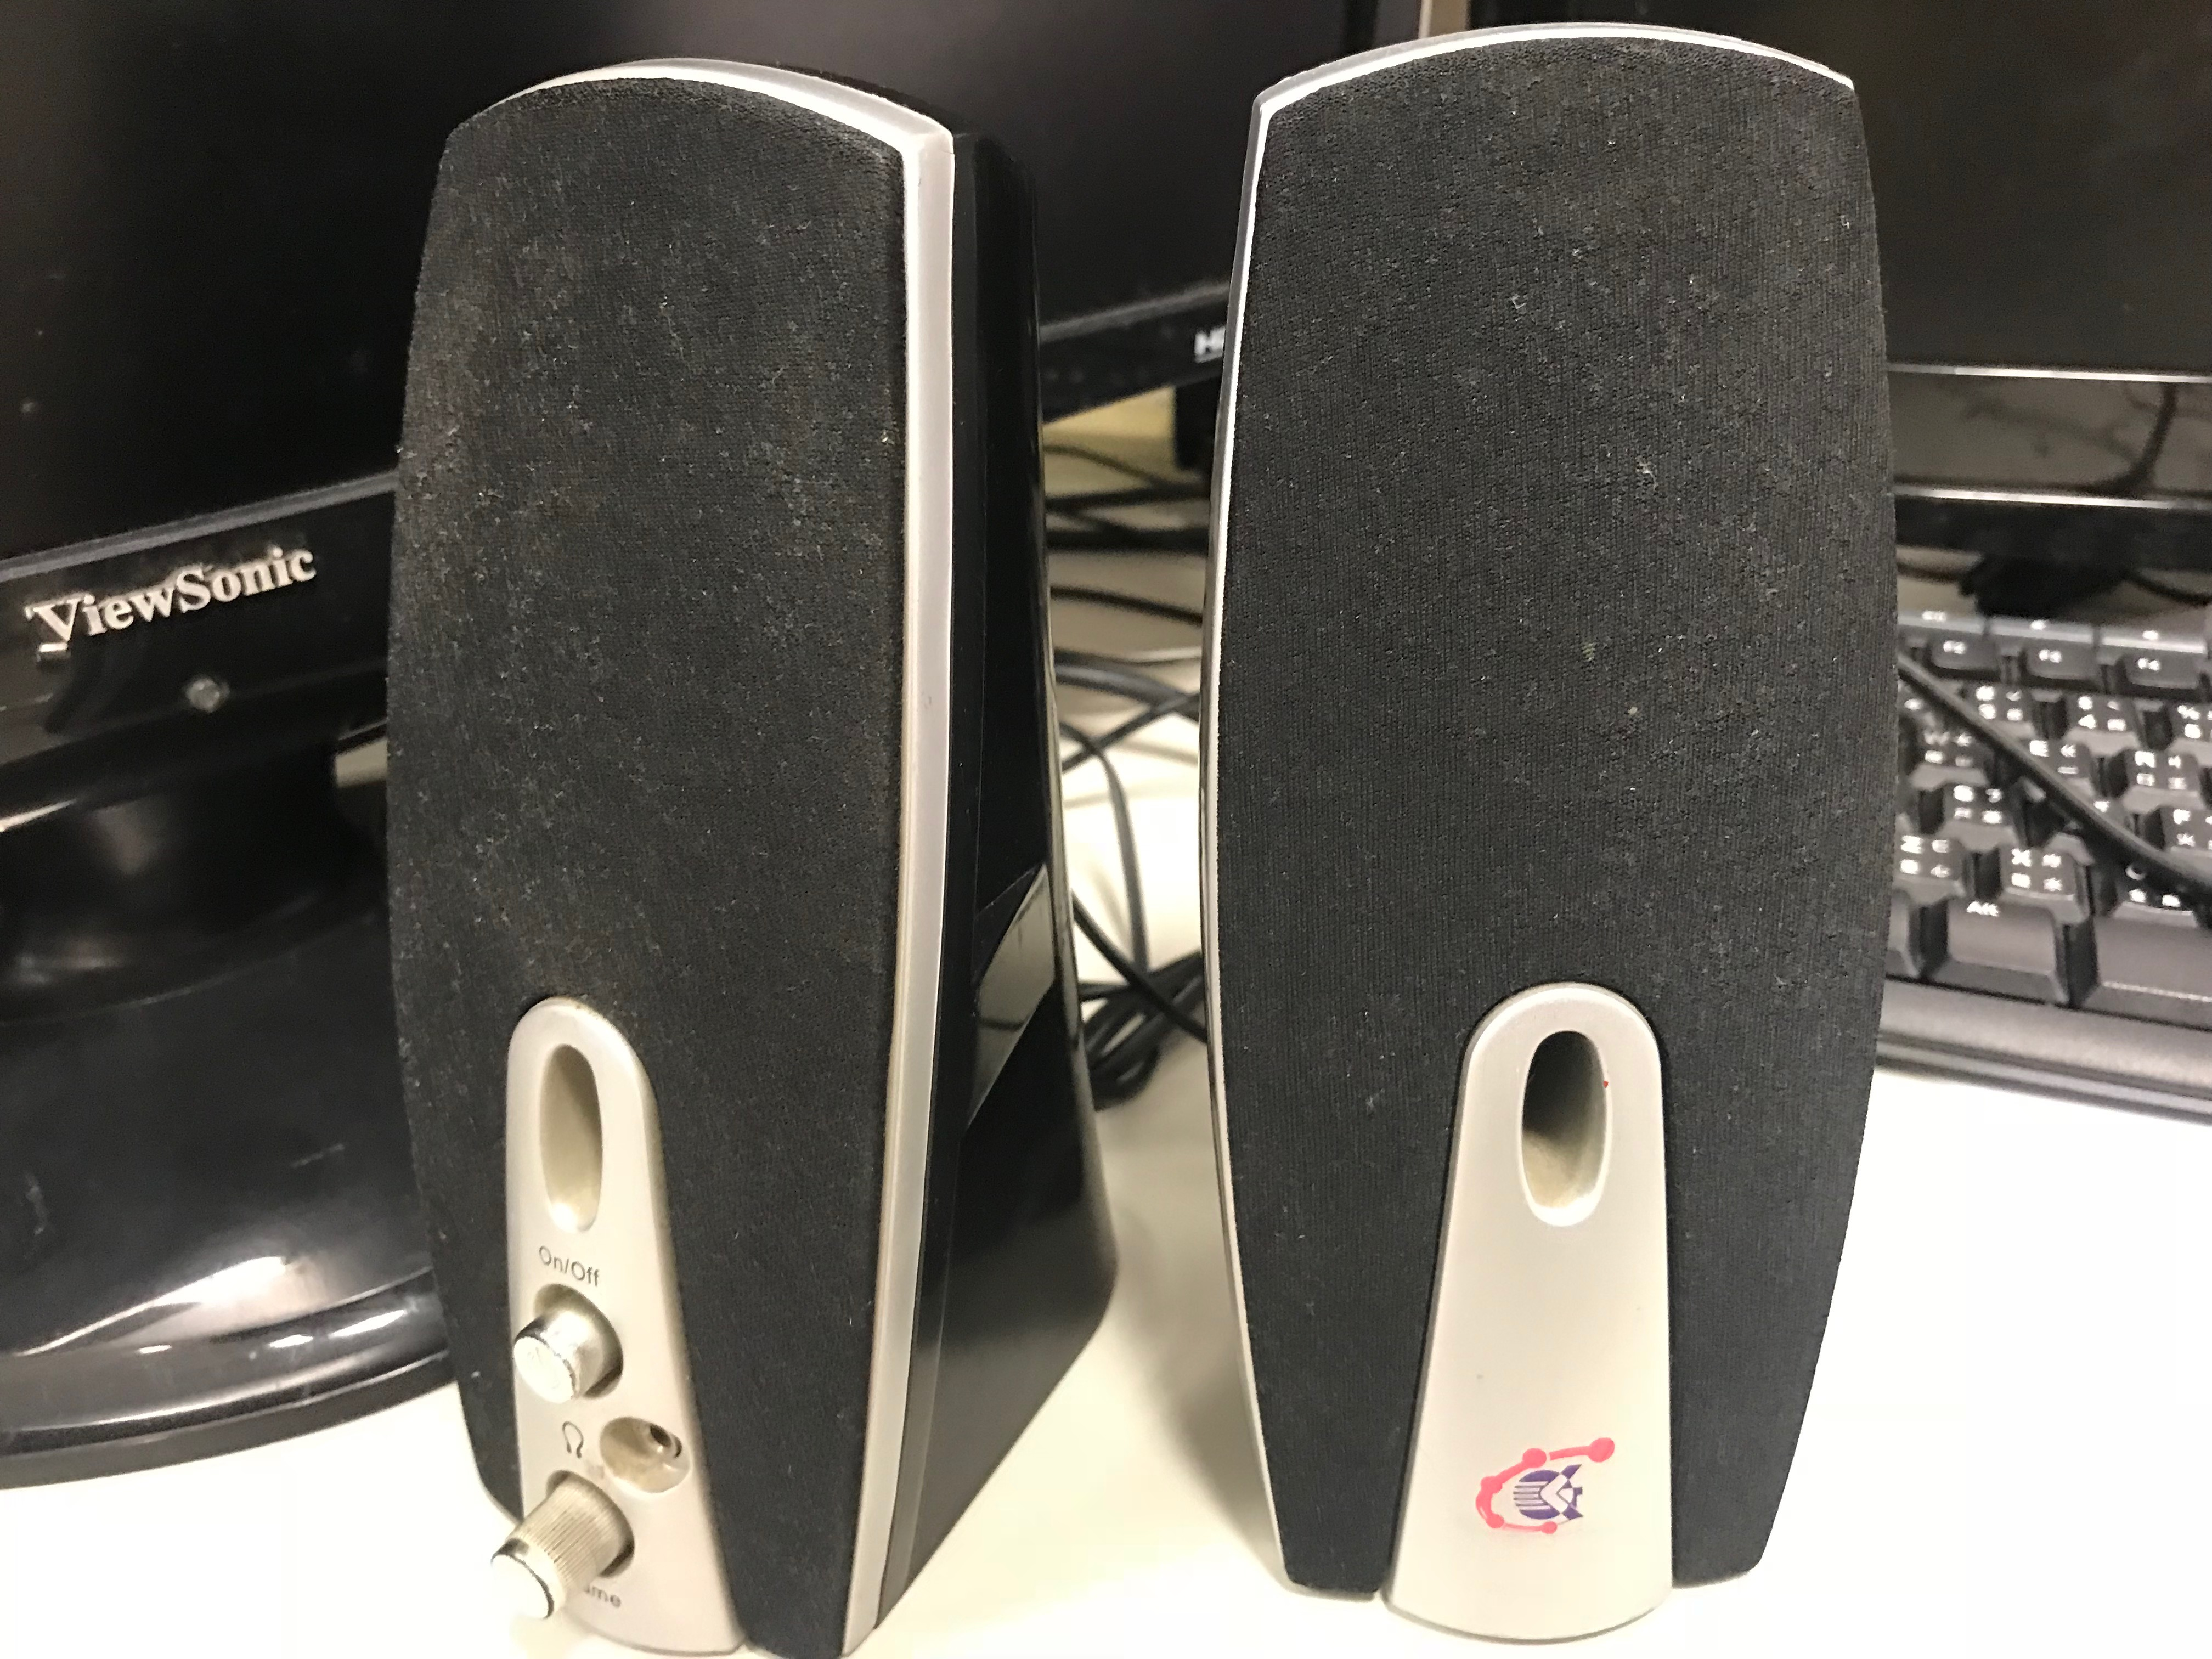
\includegraphics[width=0.6\textwidth]{img/4_pic_speaker}
  \caption{Speaker}
\end{figure}

\clearpage

\subsection{Monitor}
\begin{figure}[h]
  \centering
  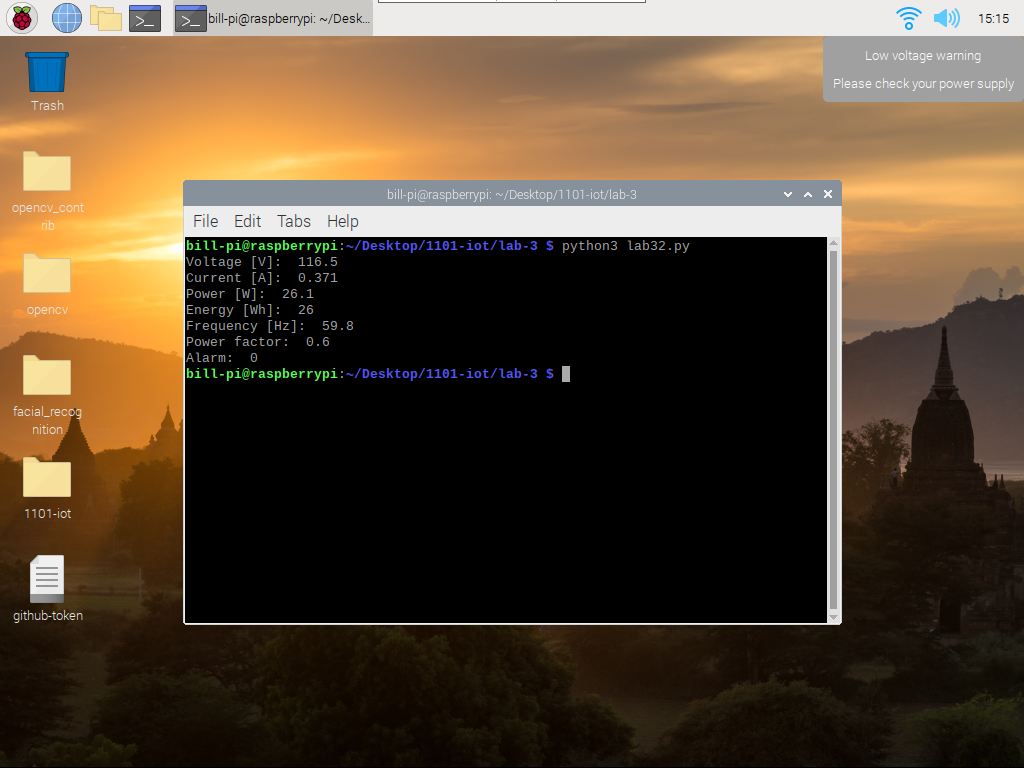
\includegraphics[width=0.6\textwidth]{img/5_res_monitor}
  \caption{Monitor result}
\end{figure}
\begin{figure}[h]
  \centering
  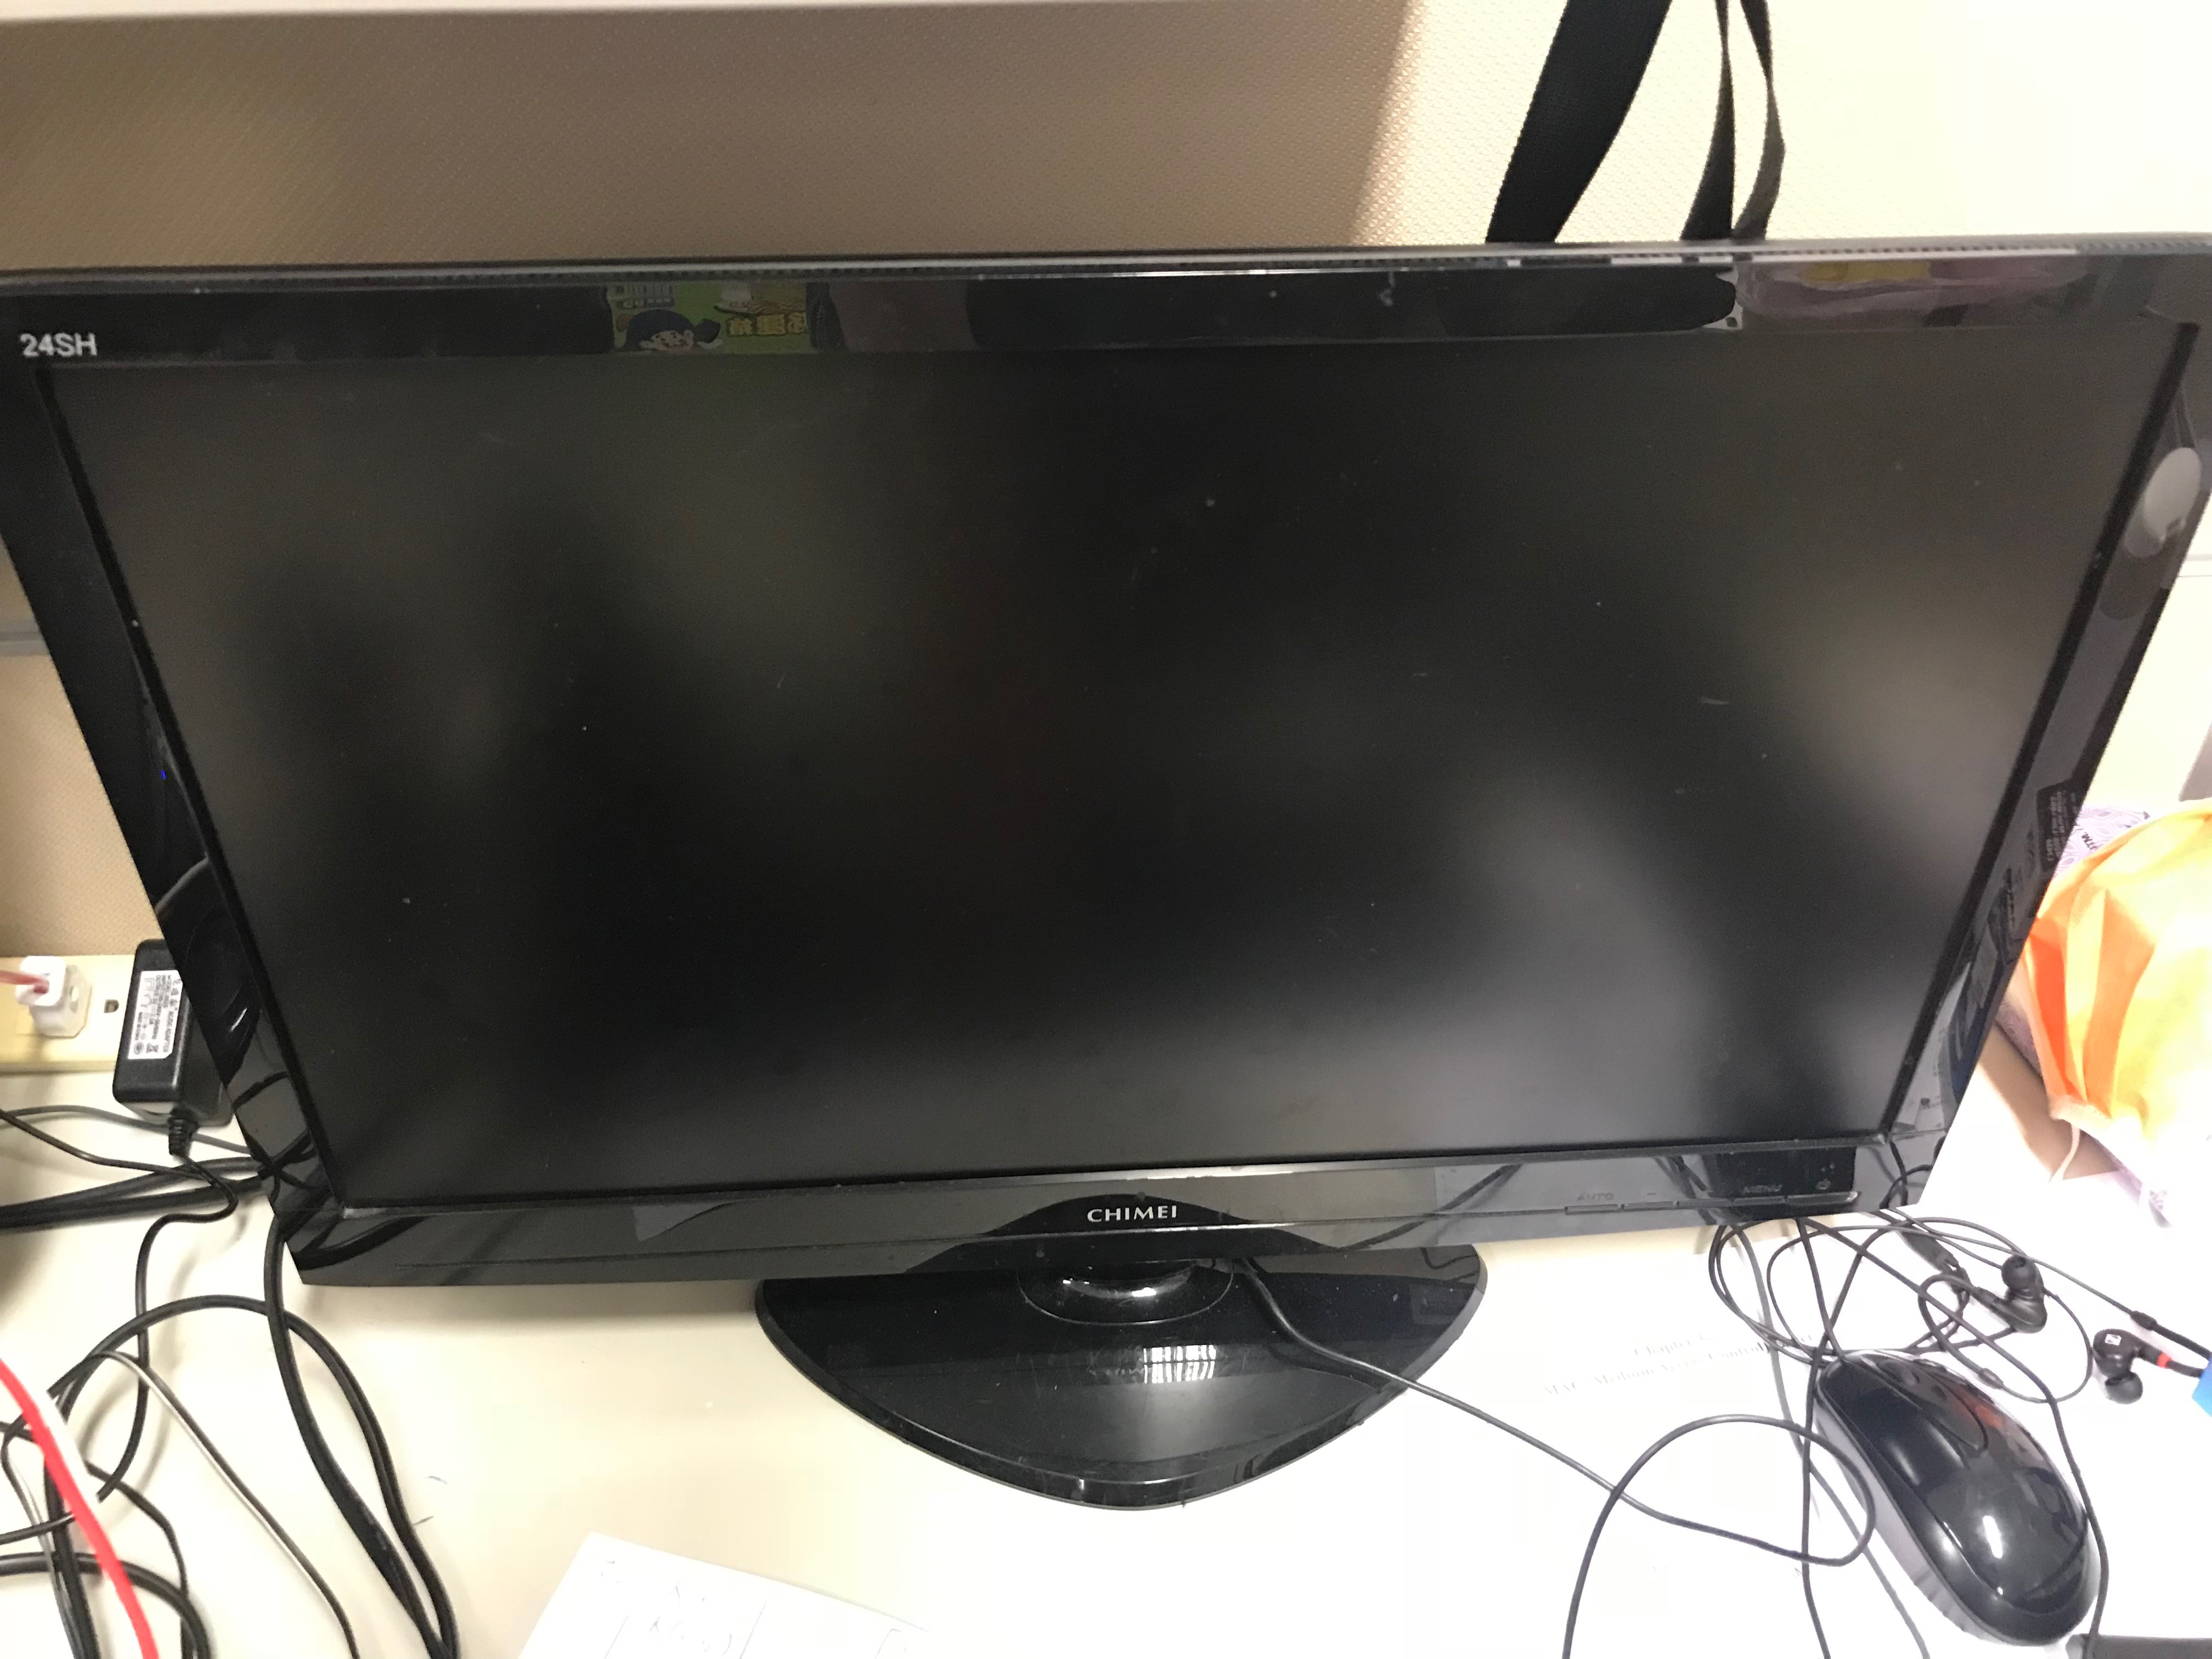
\includegraphics[width=0.6\textwidth]{img/5_pic_monitor}
  \caption{Monitor}
\end{figure}

\clearpage

\subsection{Microwave}
\begin{figure}[h]
  \centering
  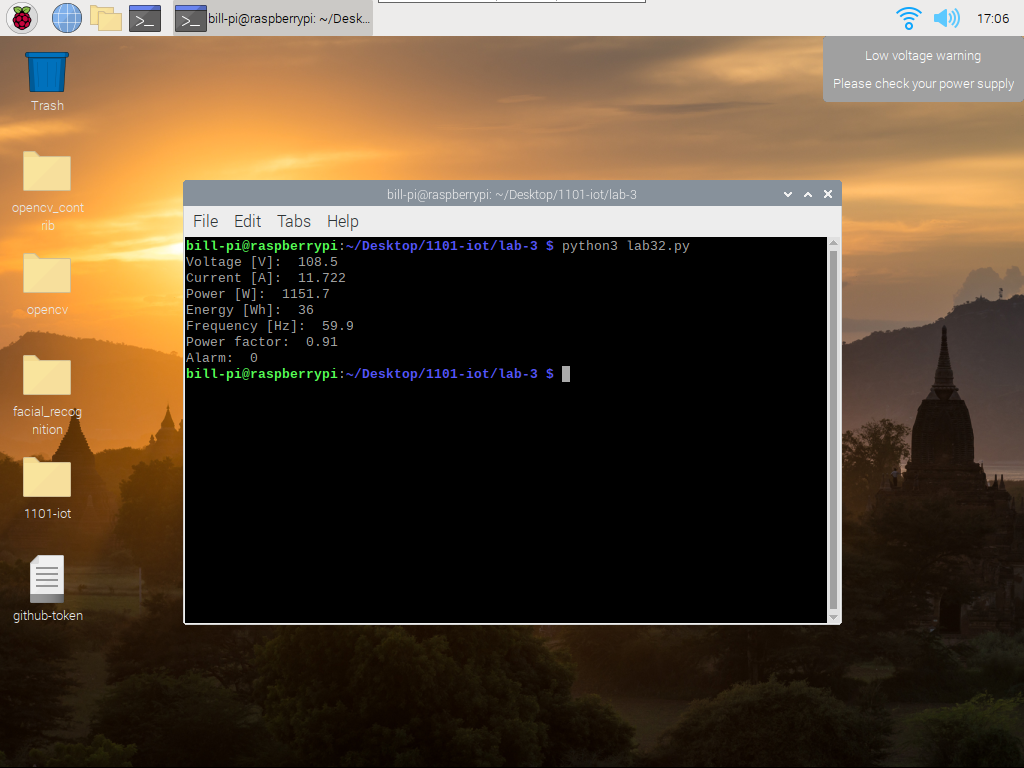
\includegraphics[width=0.6\textwidth]{img/6_res_microwave}
  \caption{Microwave result}
\end{figure}
\begin{figure}[h]
  \centering
  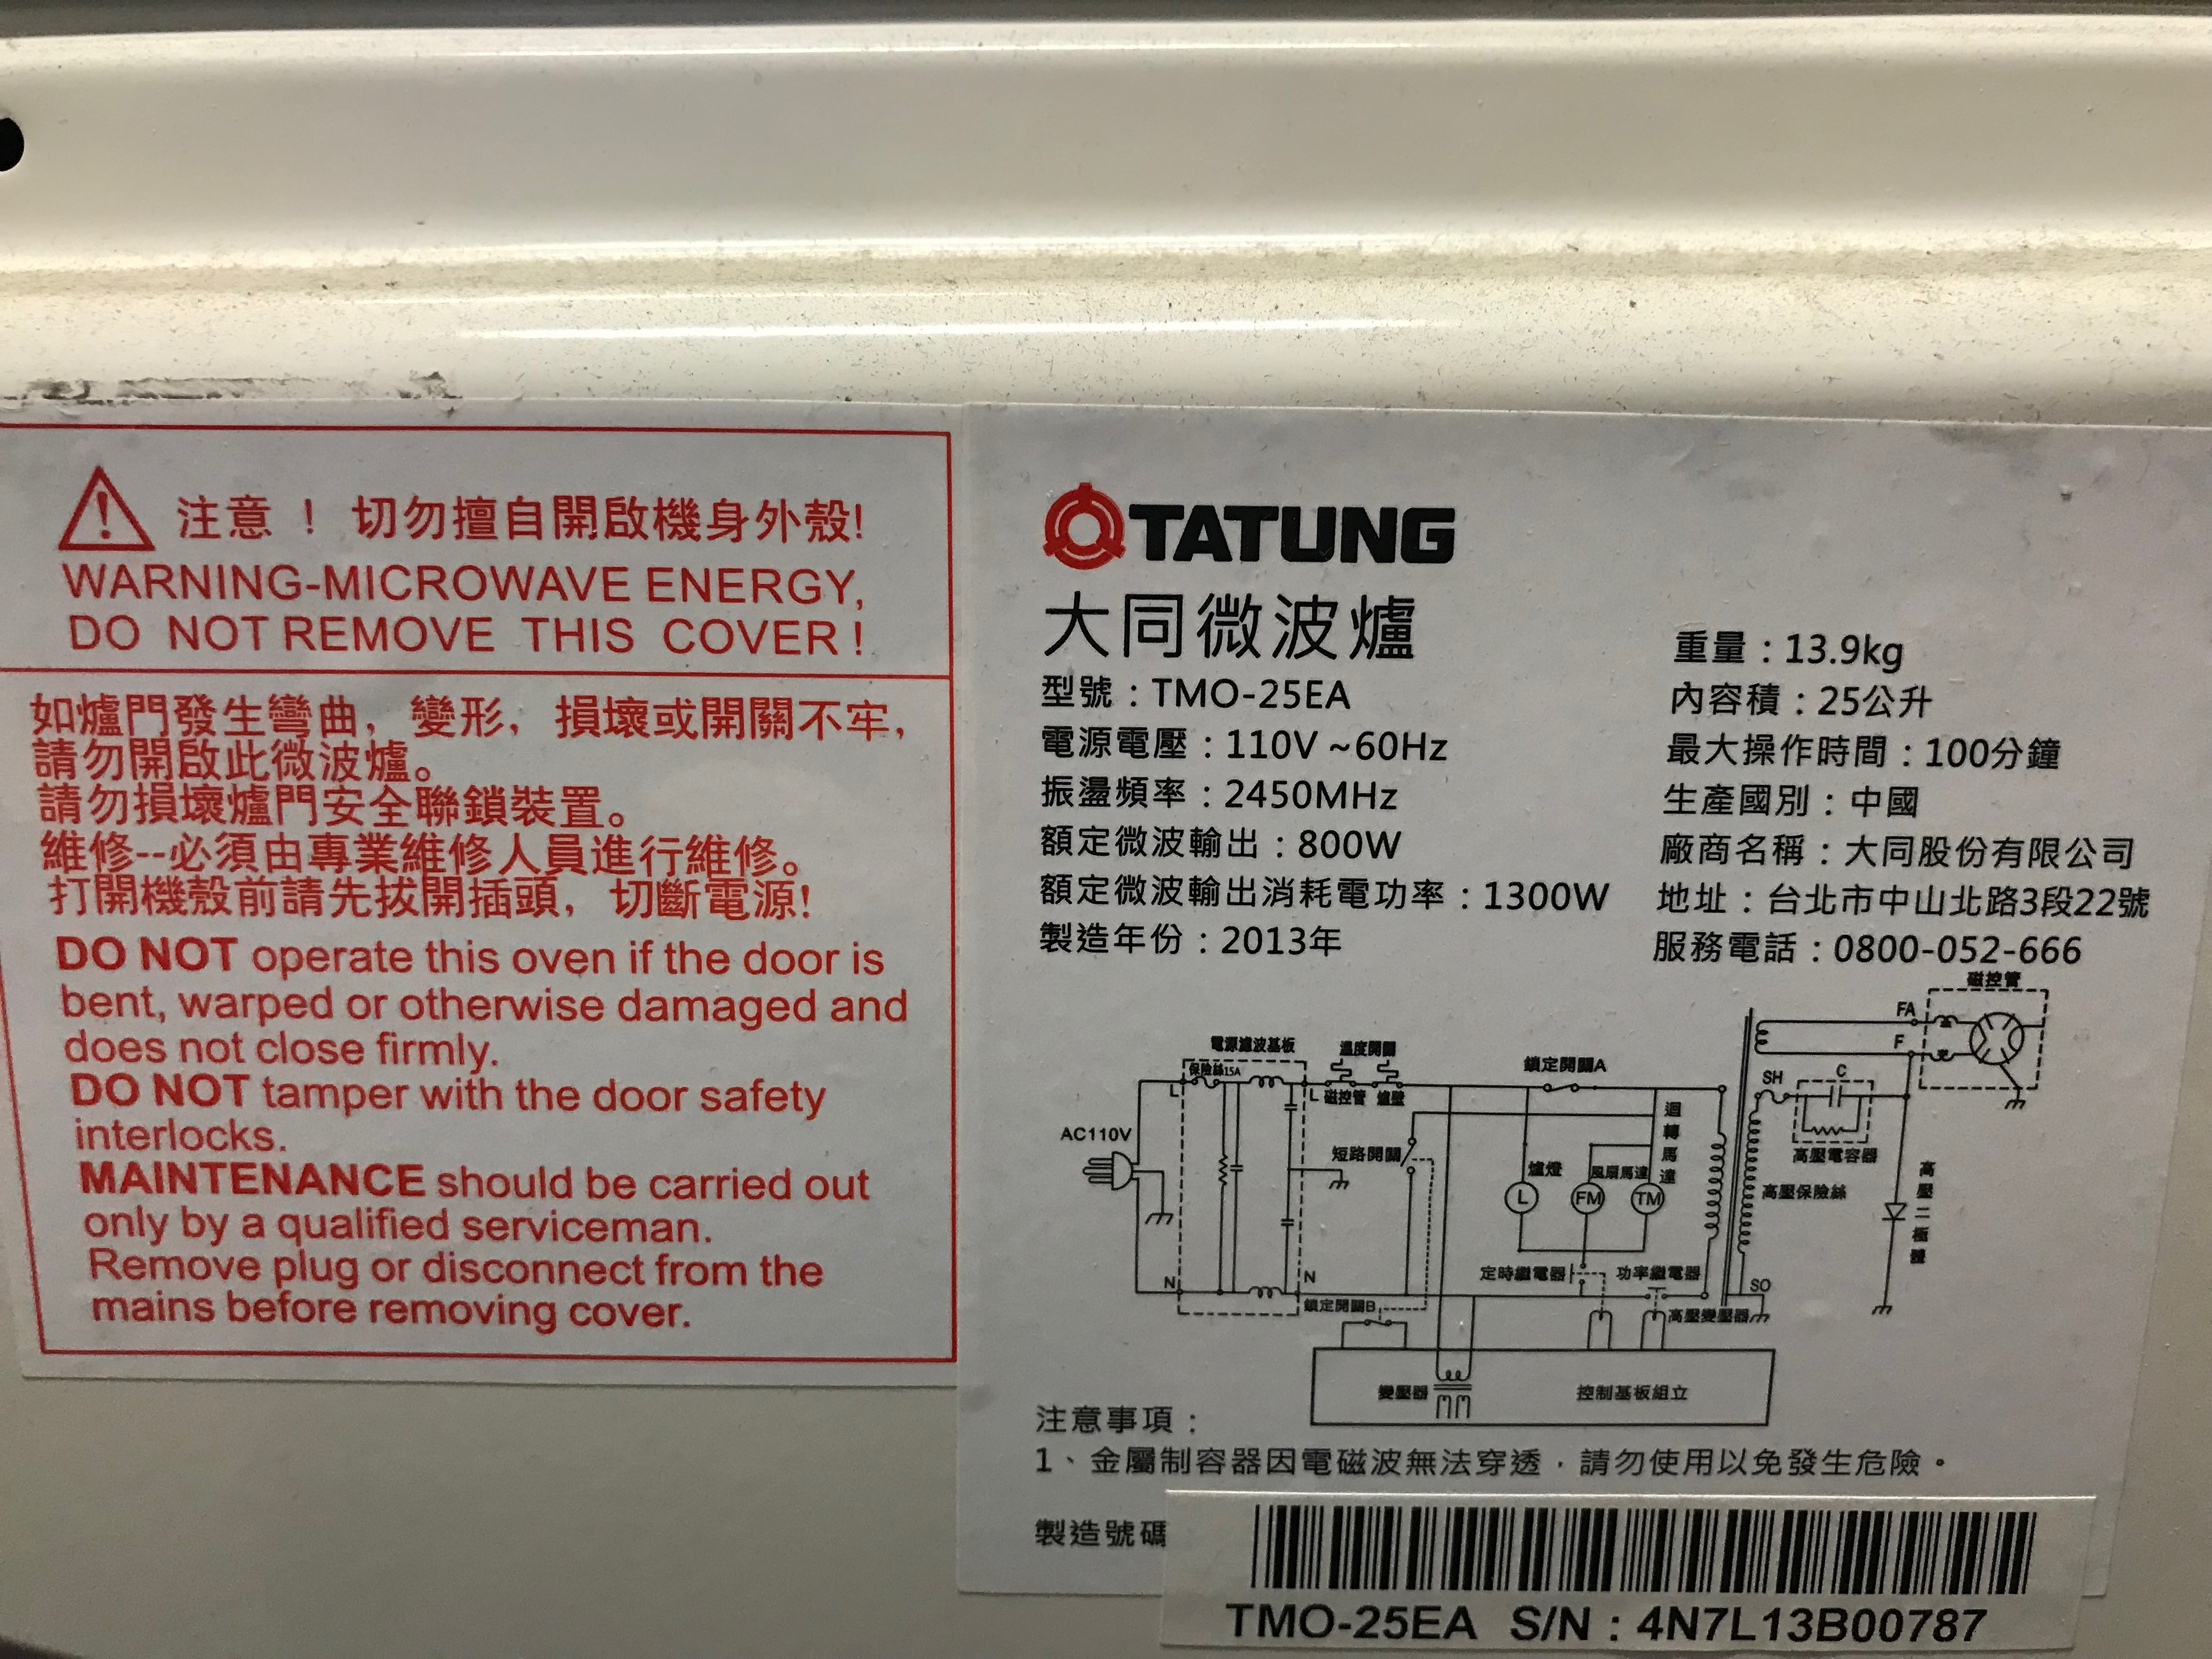
\includegraphics[width=0.6\textwidth]{img/6_spe_microwave}
  \caption{Microwave specifications}
\end{figure}
\begin{figure}[h]
  \centering
  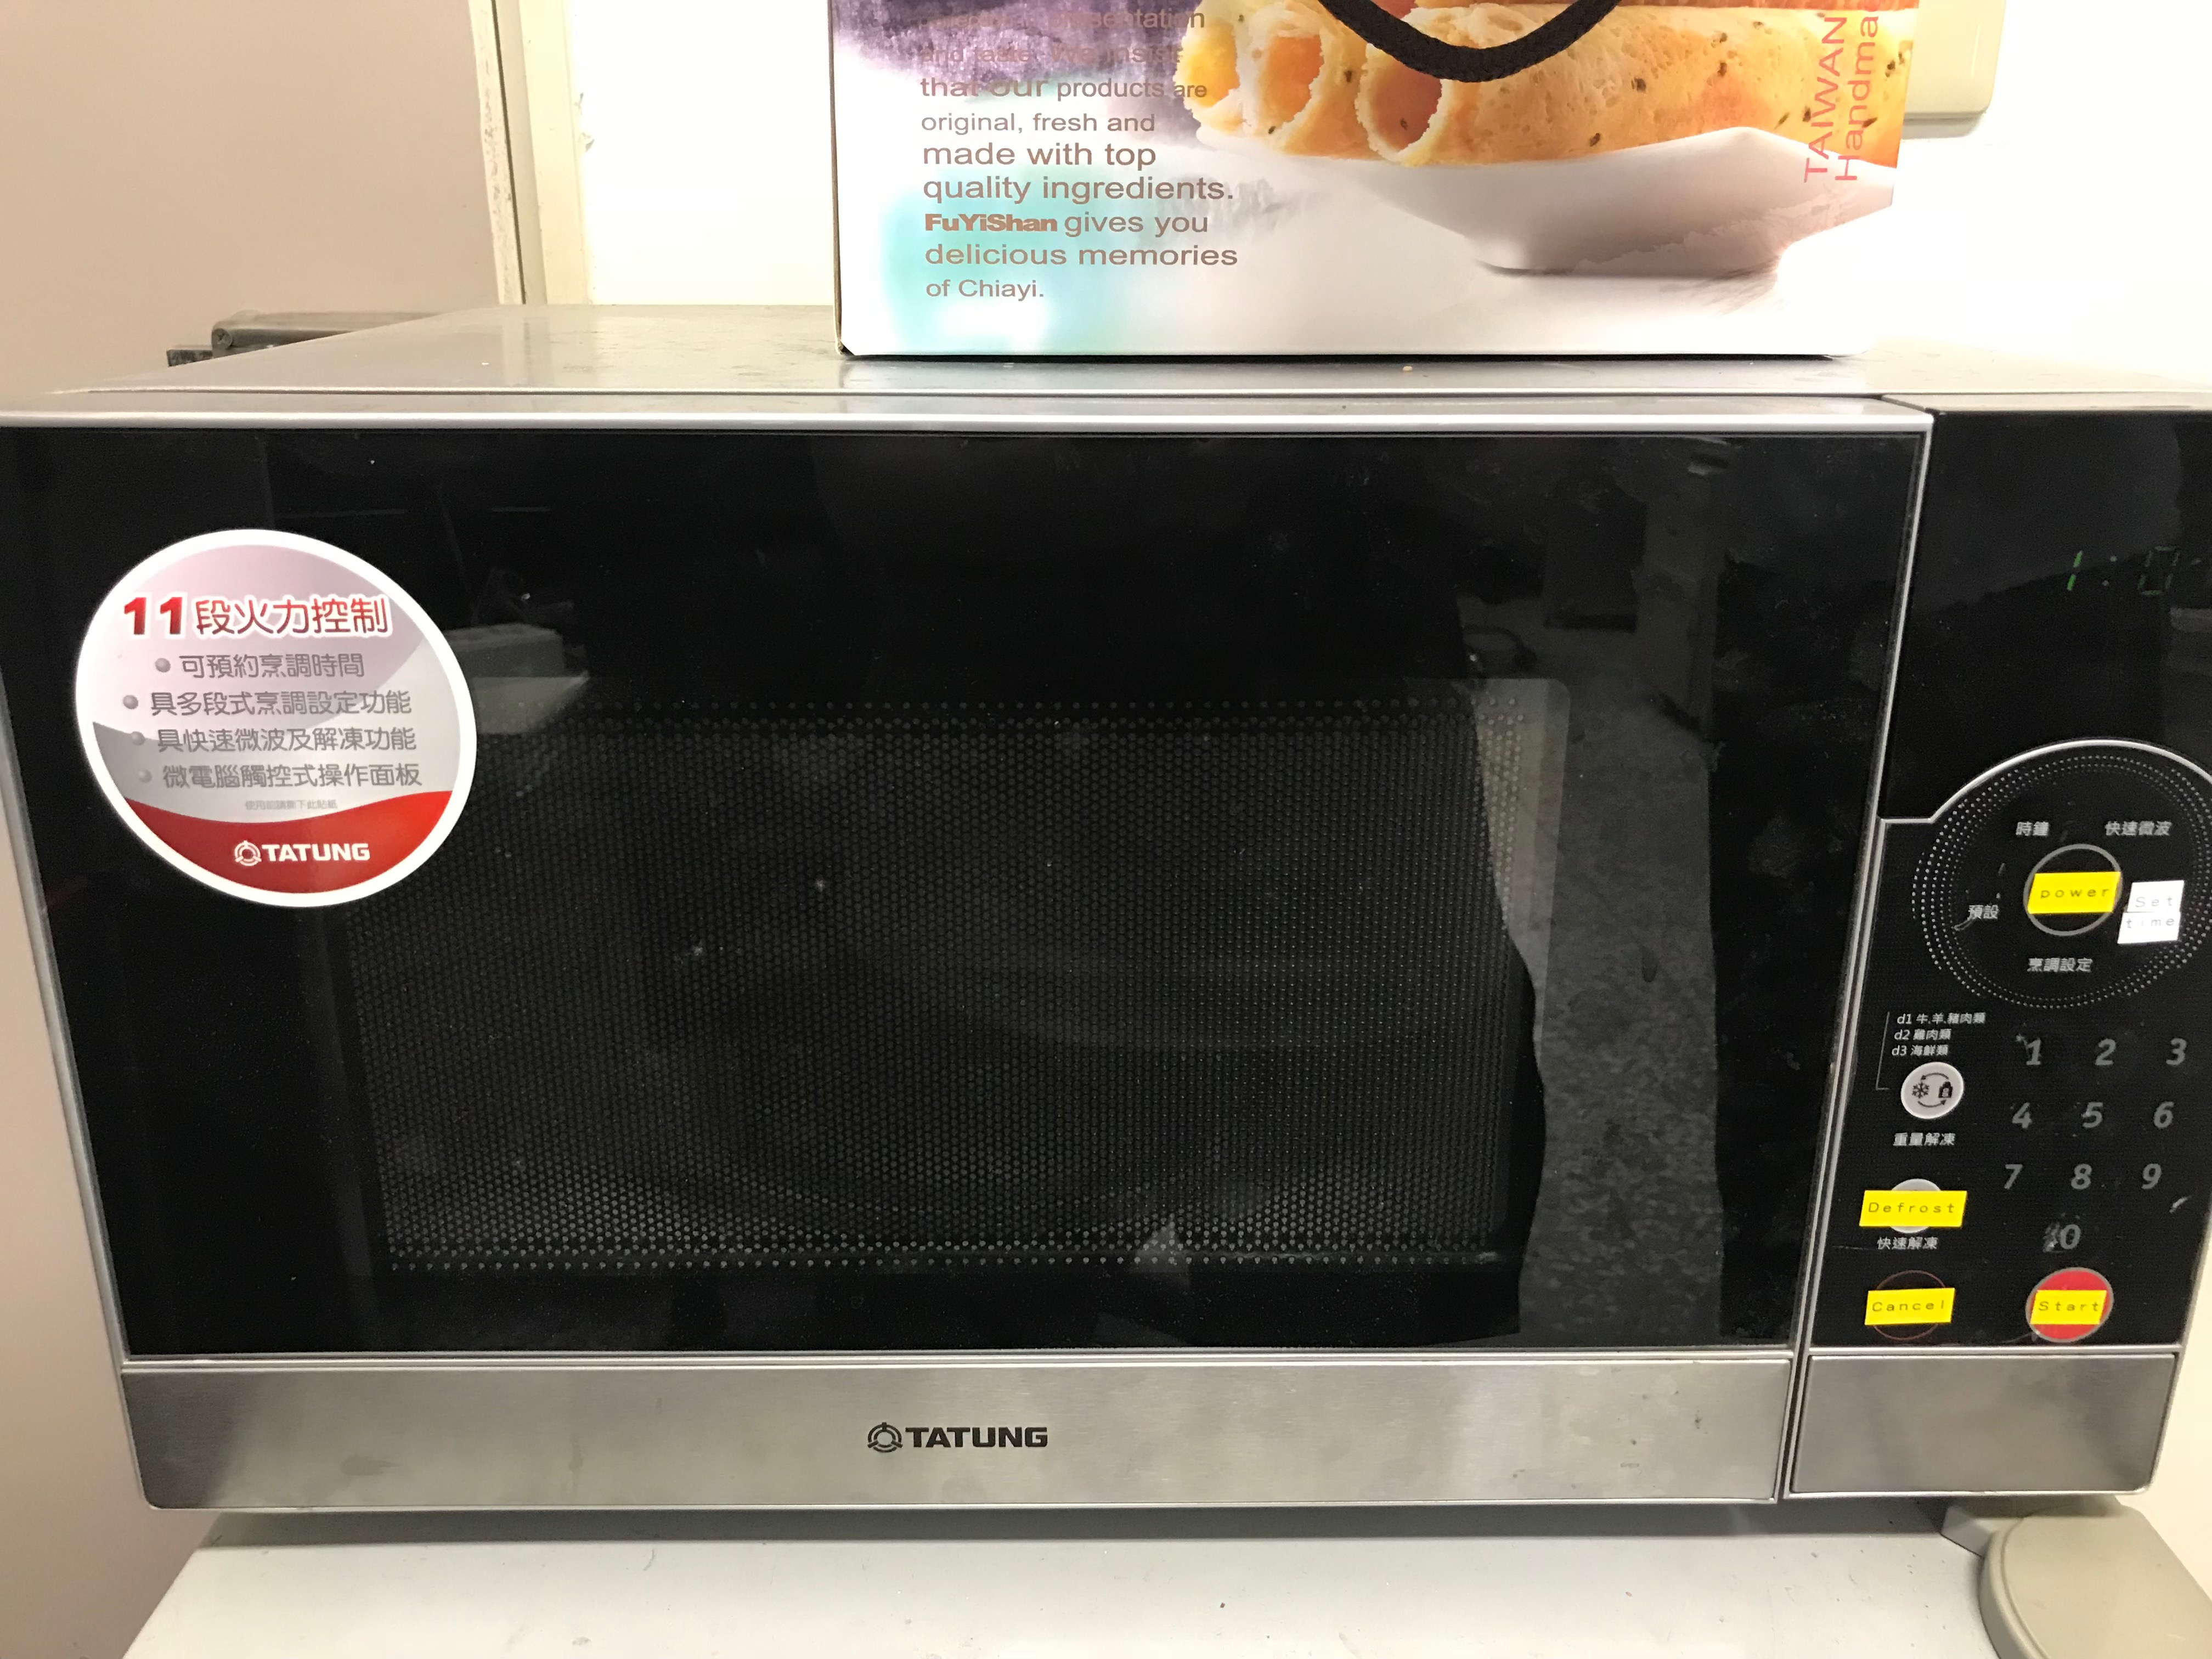
\includegraphics[width=0.6\textwidth]{img/6_pic_microwave}
  \caption{Microwave}
\end{figure}

\clearpage

\subsection{Street light}
\begin{figure}[h]
  \centering
  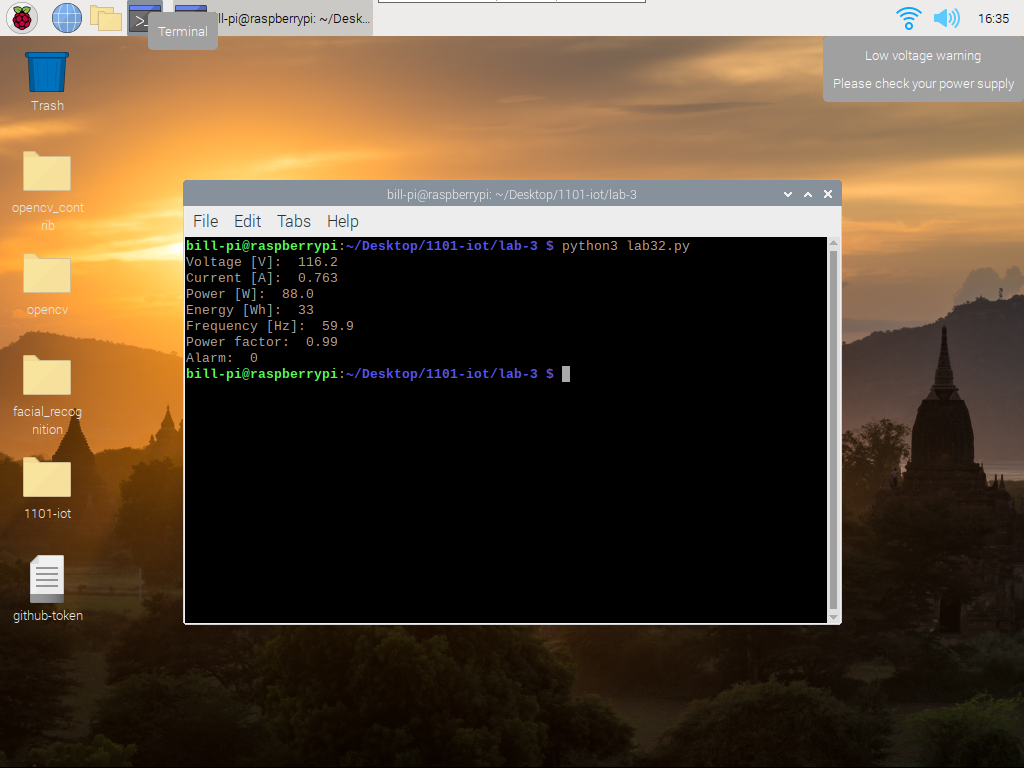
\includegraphics[width=0.6\textwidth]{img/7_res_street_light}
  \caption{Street light result}
\end{figure}
\begin{figure}[h]
  \centering
  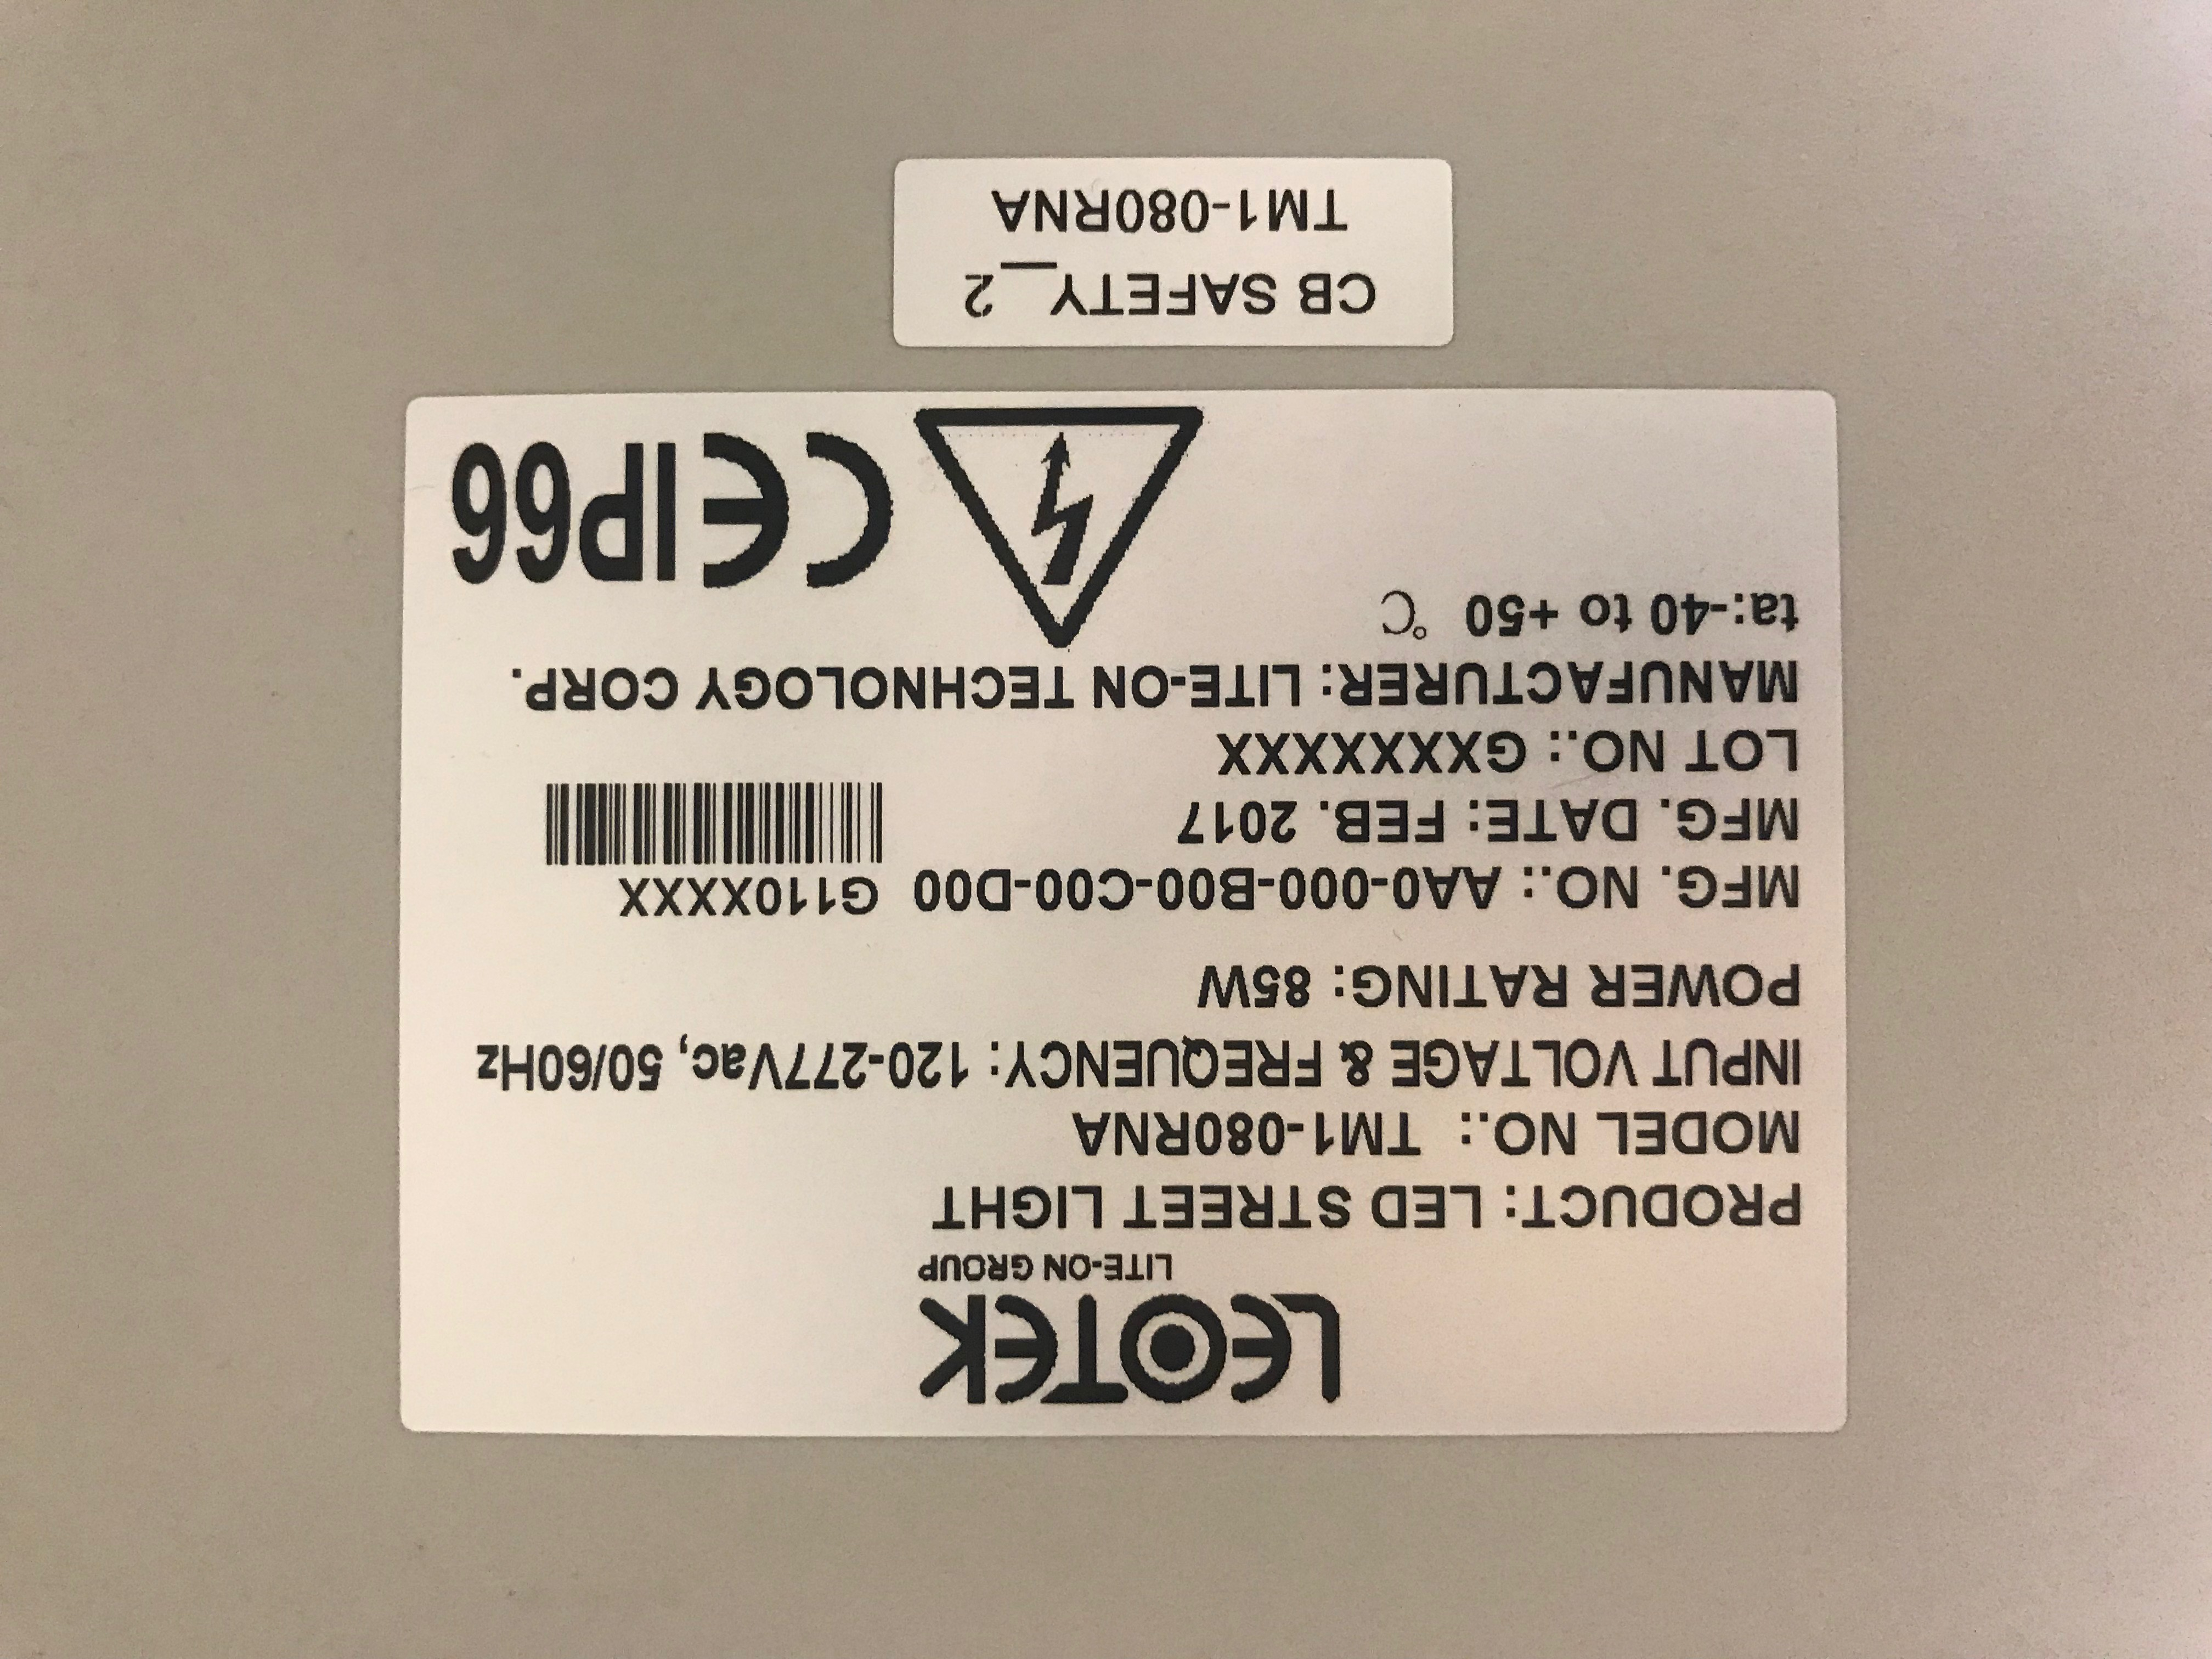
\includegraphics[angle=180, origin=c, width=0.6\textwidth]{img/7_spe_street_light}
  \caption{Street light specifications}
\end{figure}
\begin{figure}[h]
  \centering
  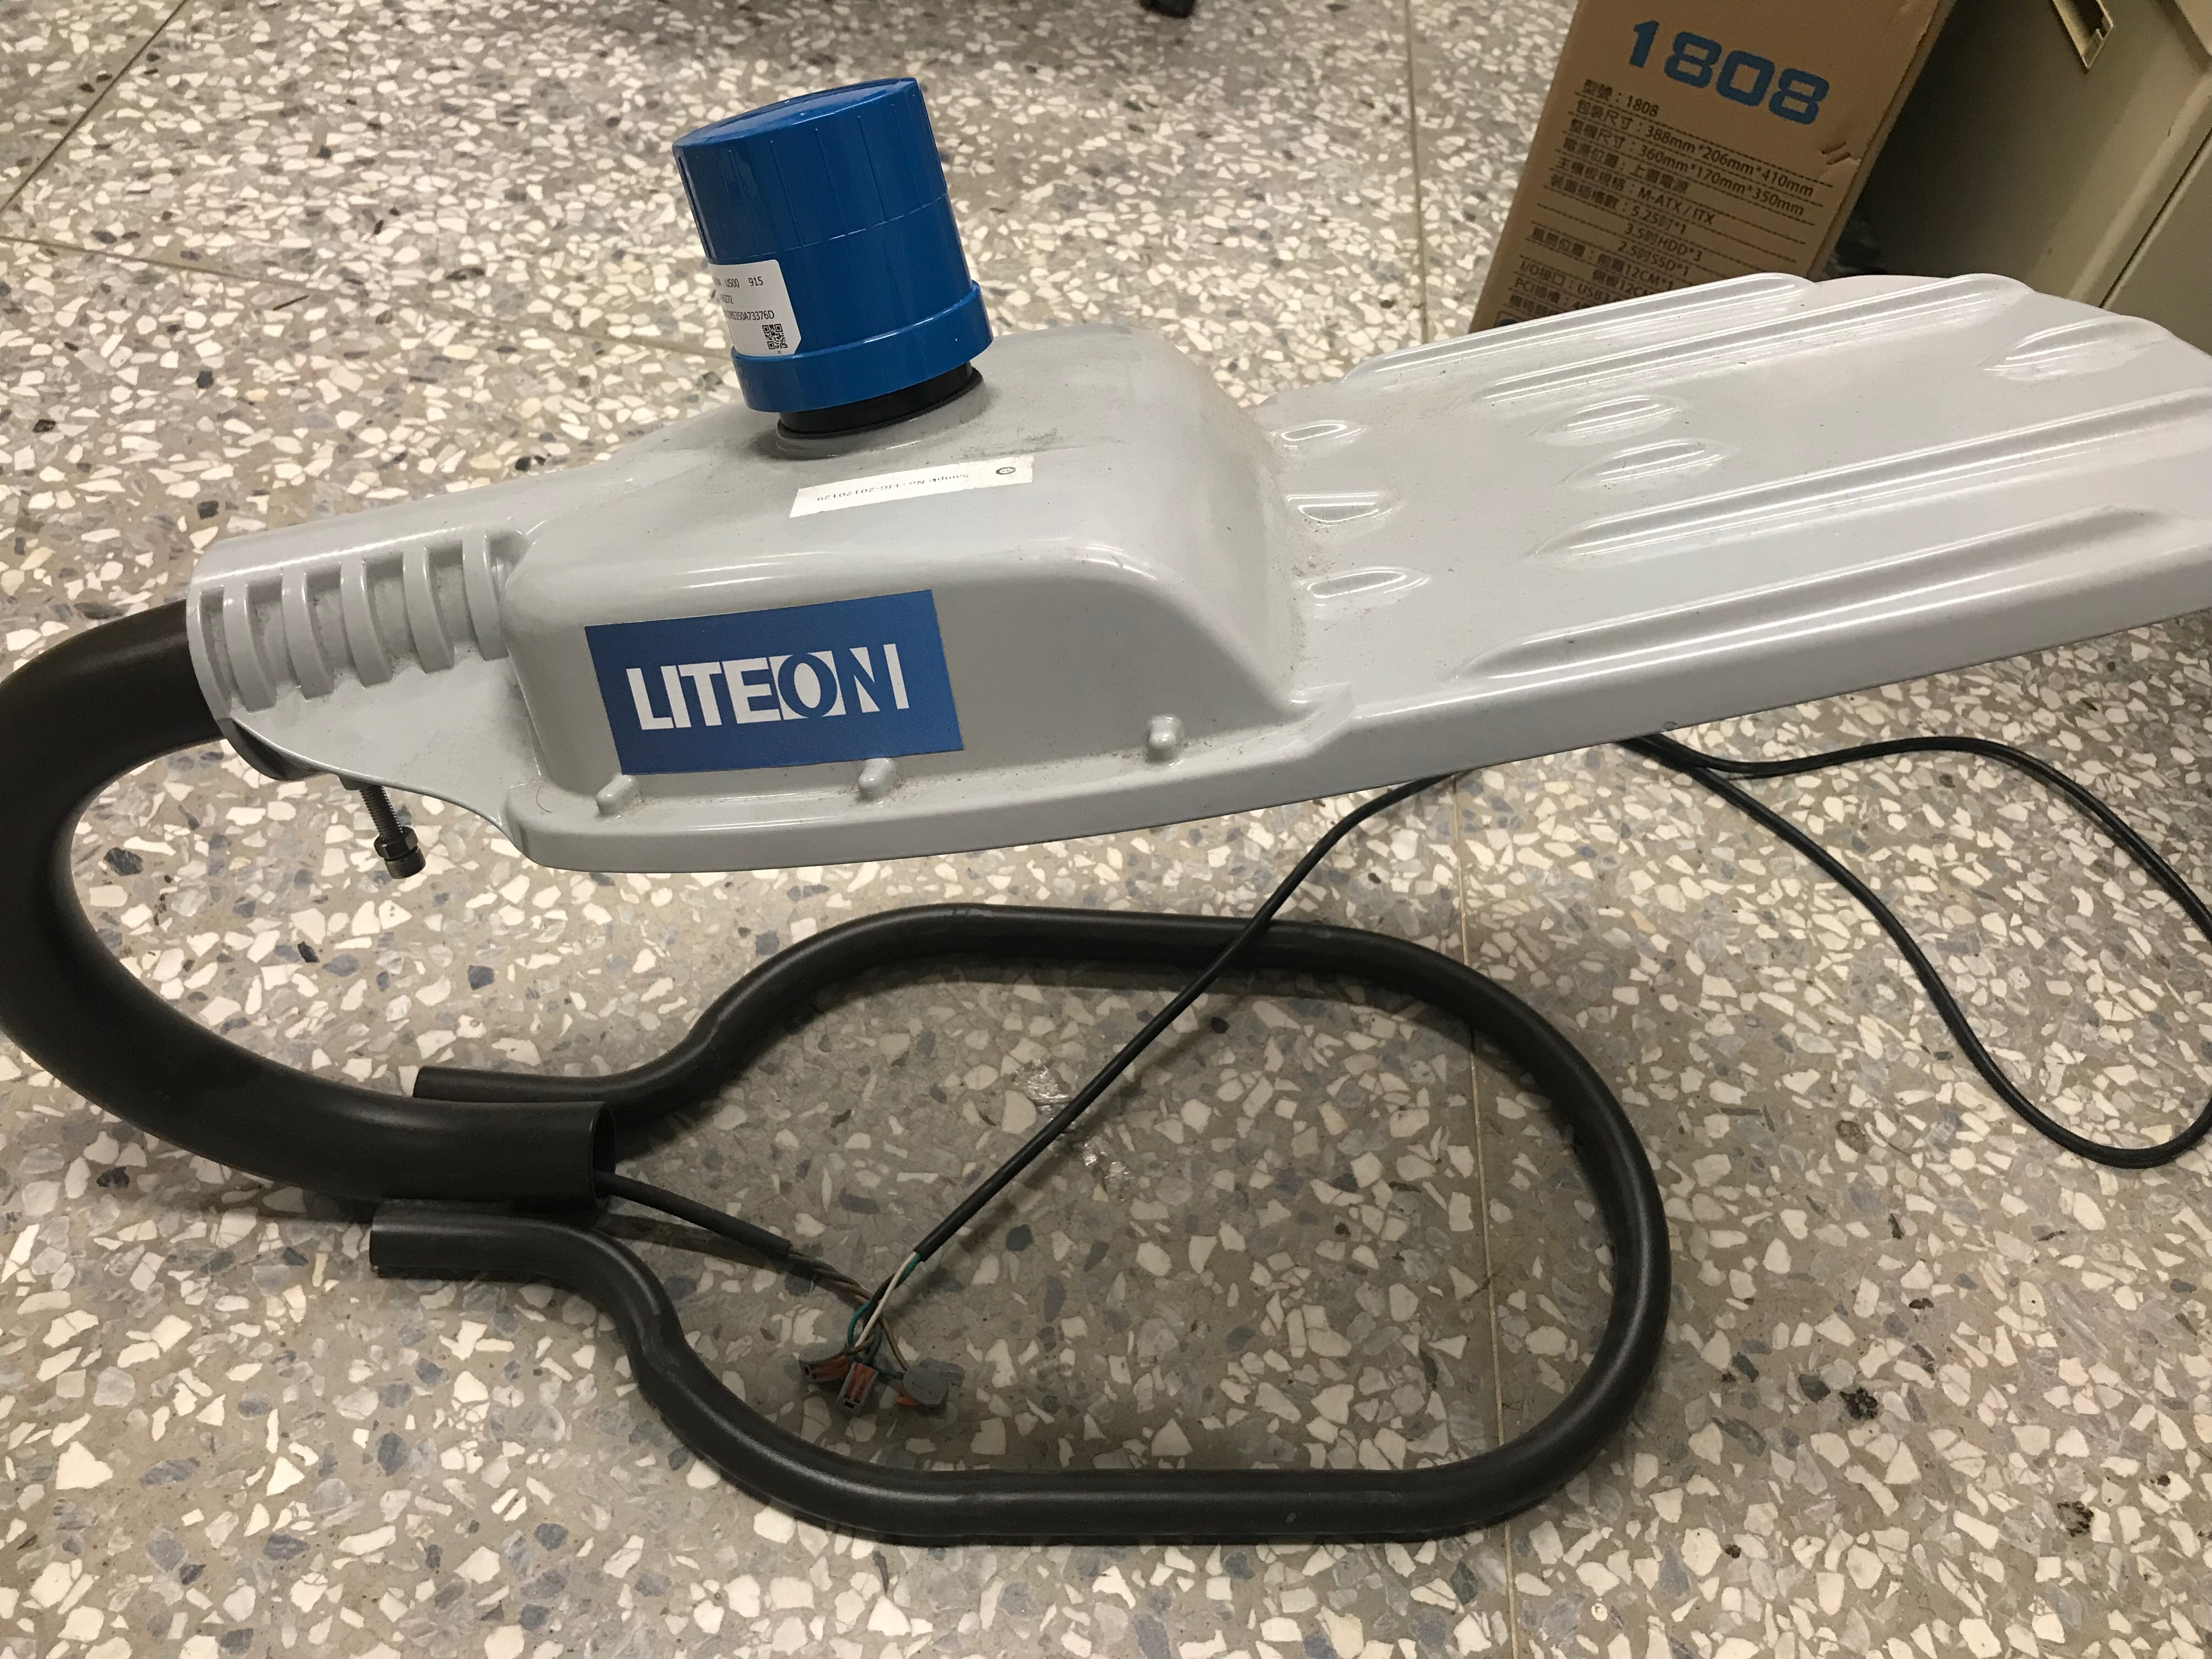
\includegraphics[width=0.6\textwidth]{img/7_pic_street_light}
  \caption{Street light}
\end{figure}

\clearpage

\subsection{Mini-monitor}
\begin{figure}[h]
  \centering
  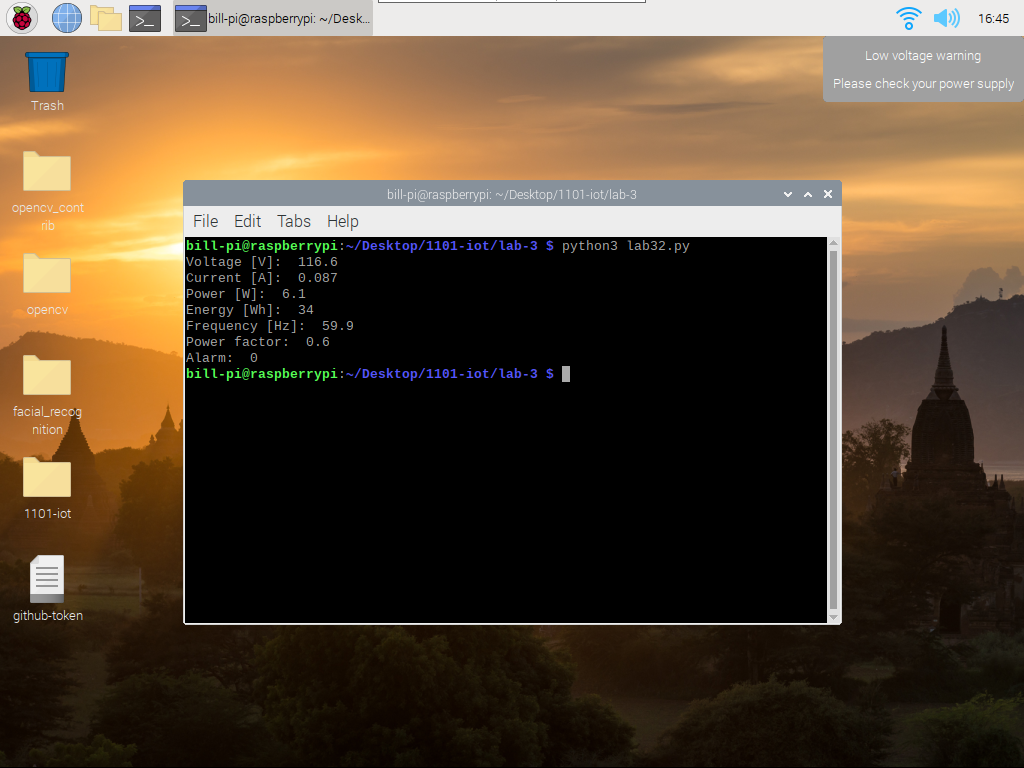
\includegraphics[width=0.6\textwidth]{img/8_res_minimonitor}
  \caption{Mini-monitor result}
\end{figure}
\begin{figure}[h]
  \centering
  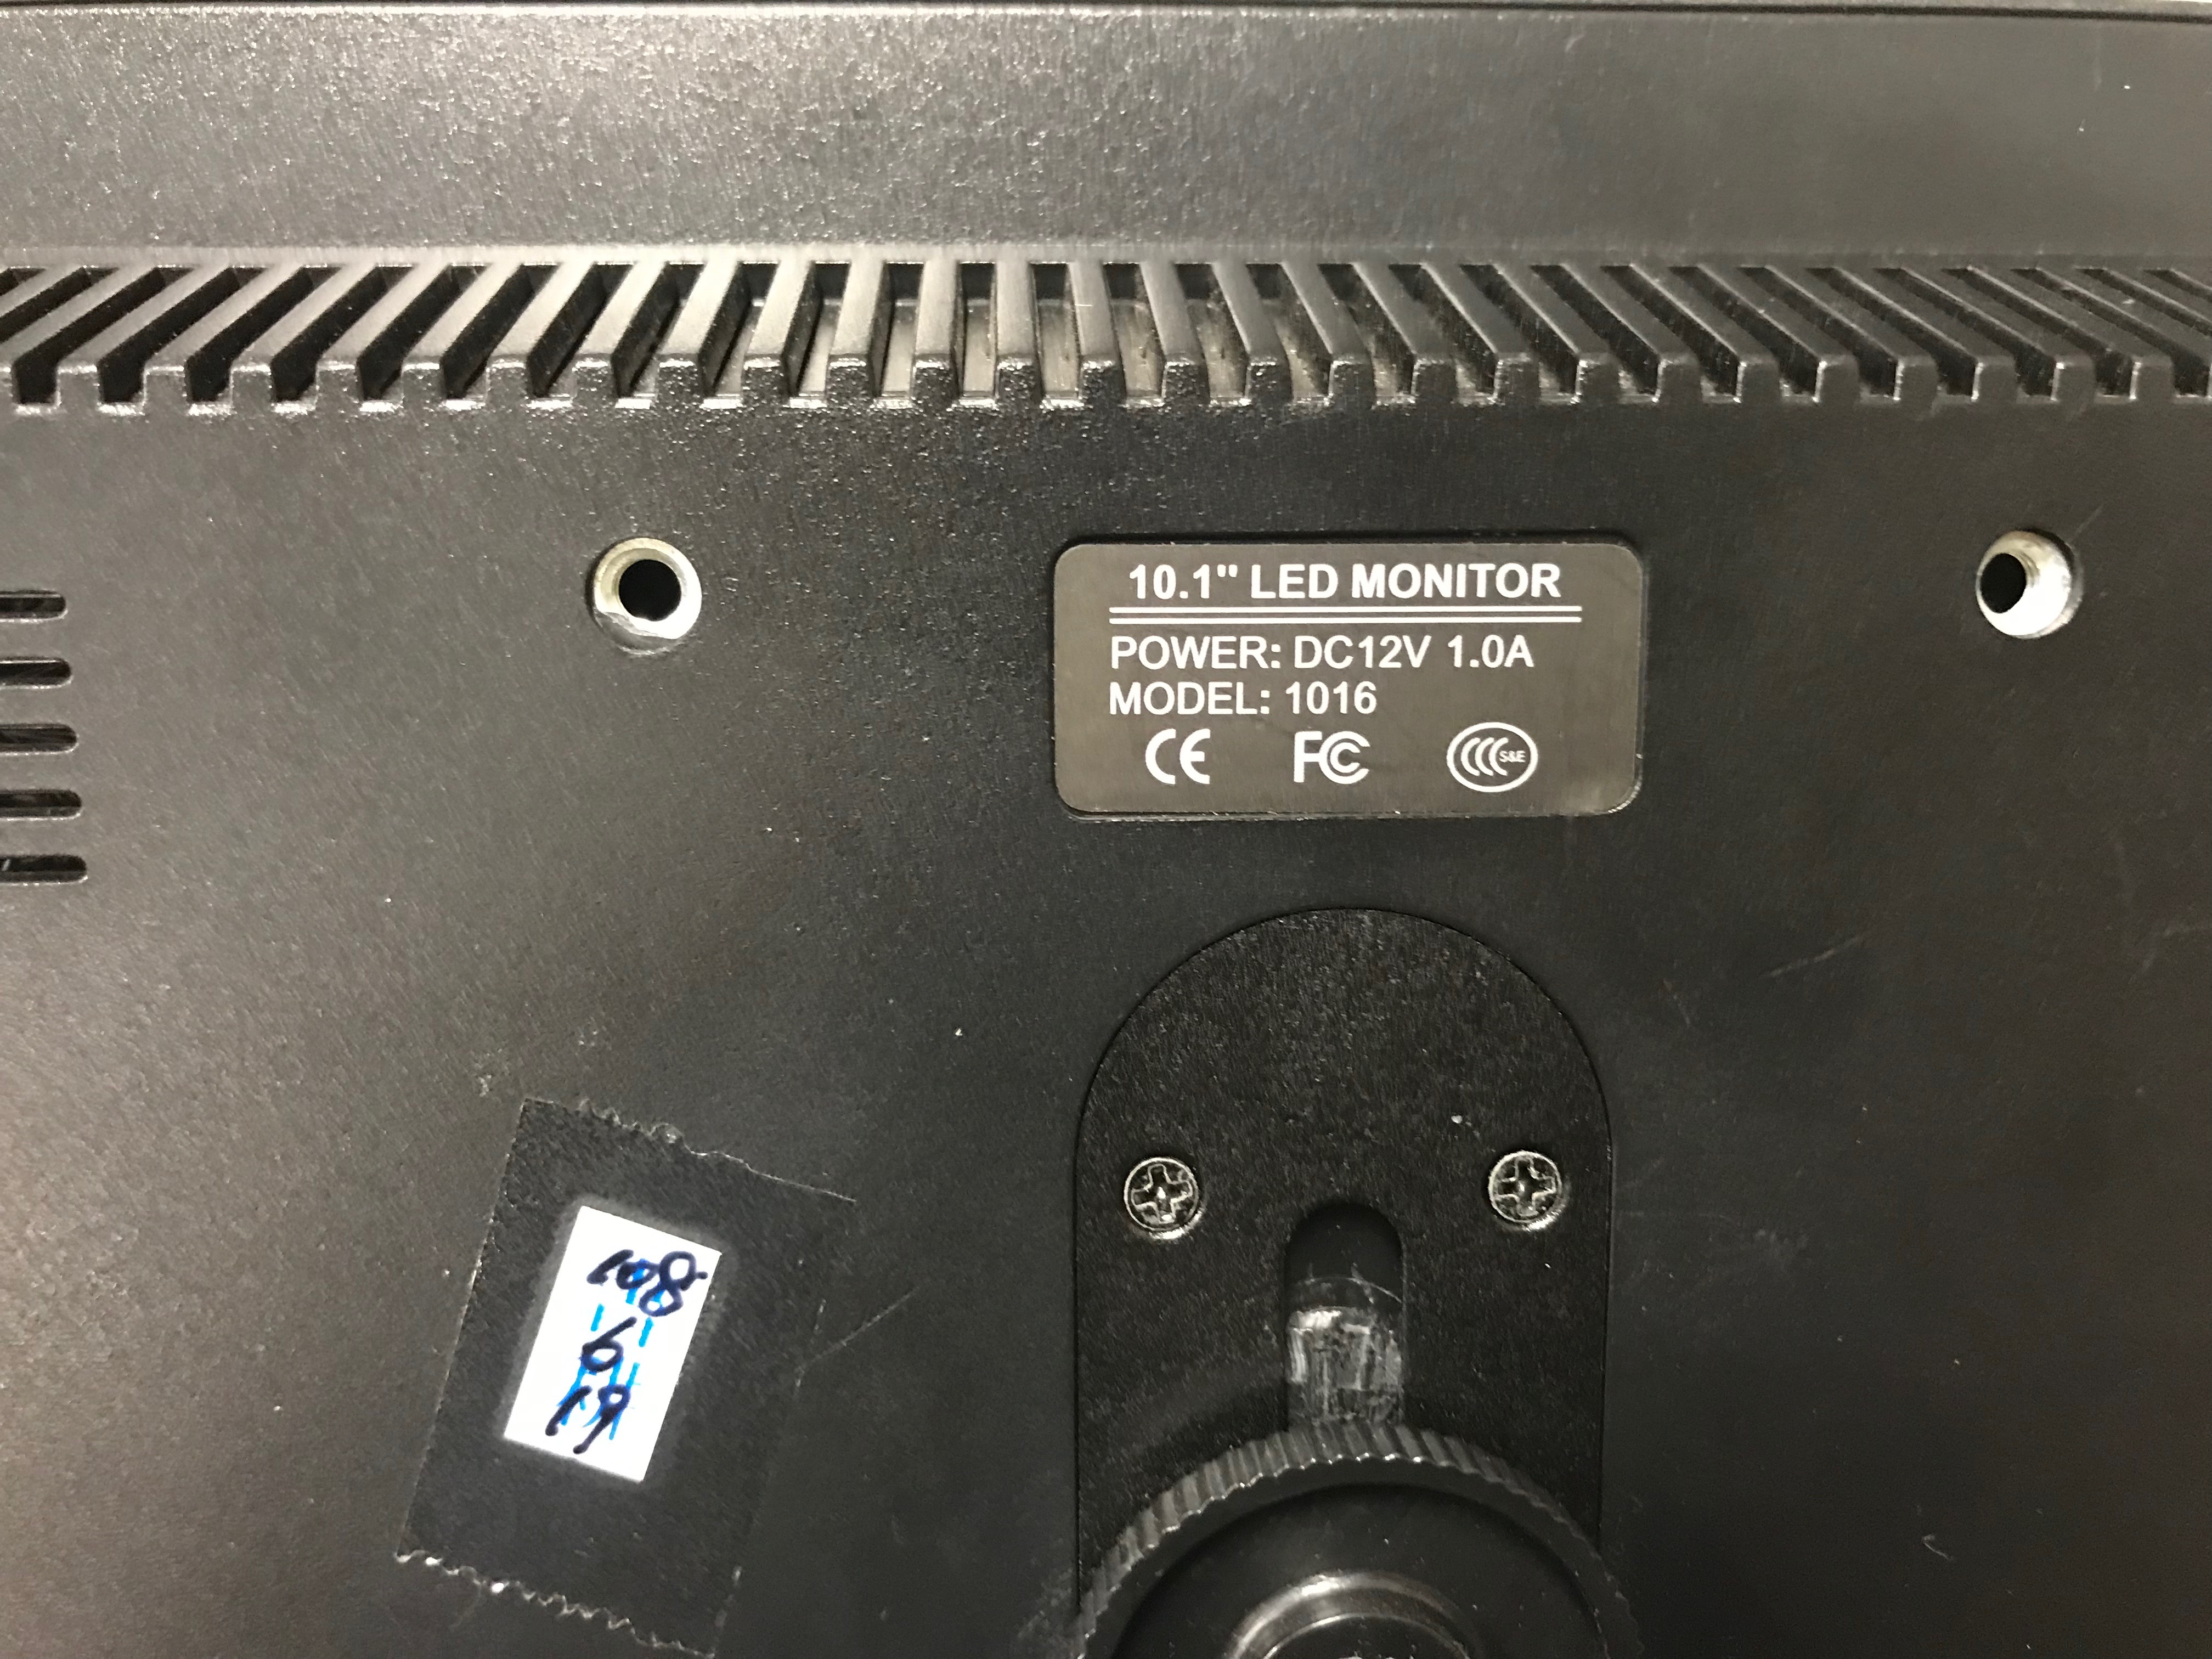
\includegraphics[width=0.6\textwidth]{img/8_spe_minimonitor}
  \caption{Mini-monitor specifications}
\end{figure}
\begin{figure}[h]
  \centering
  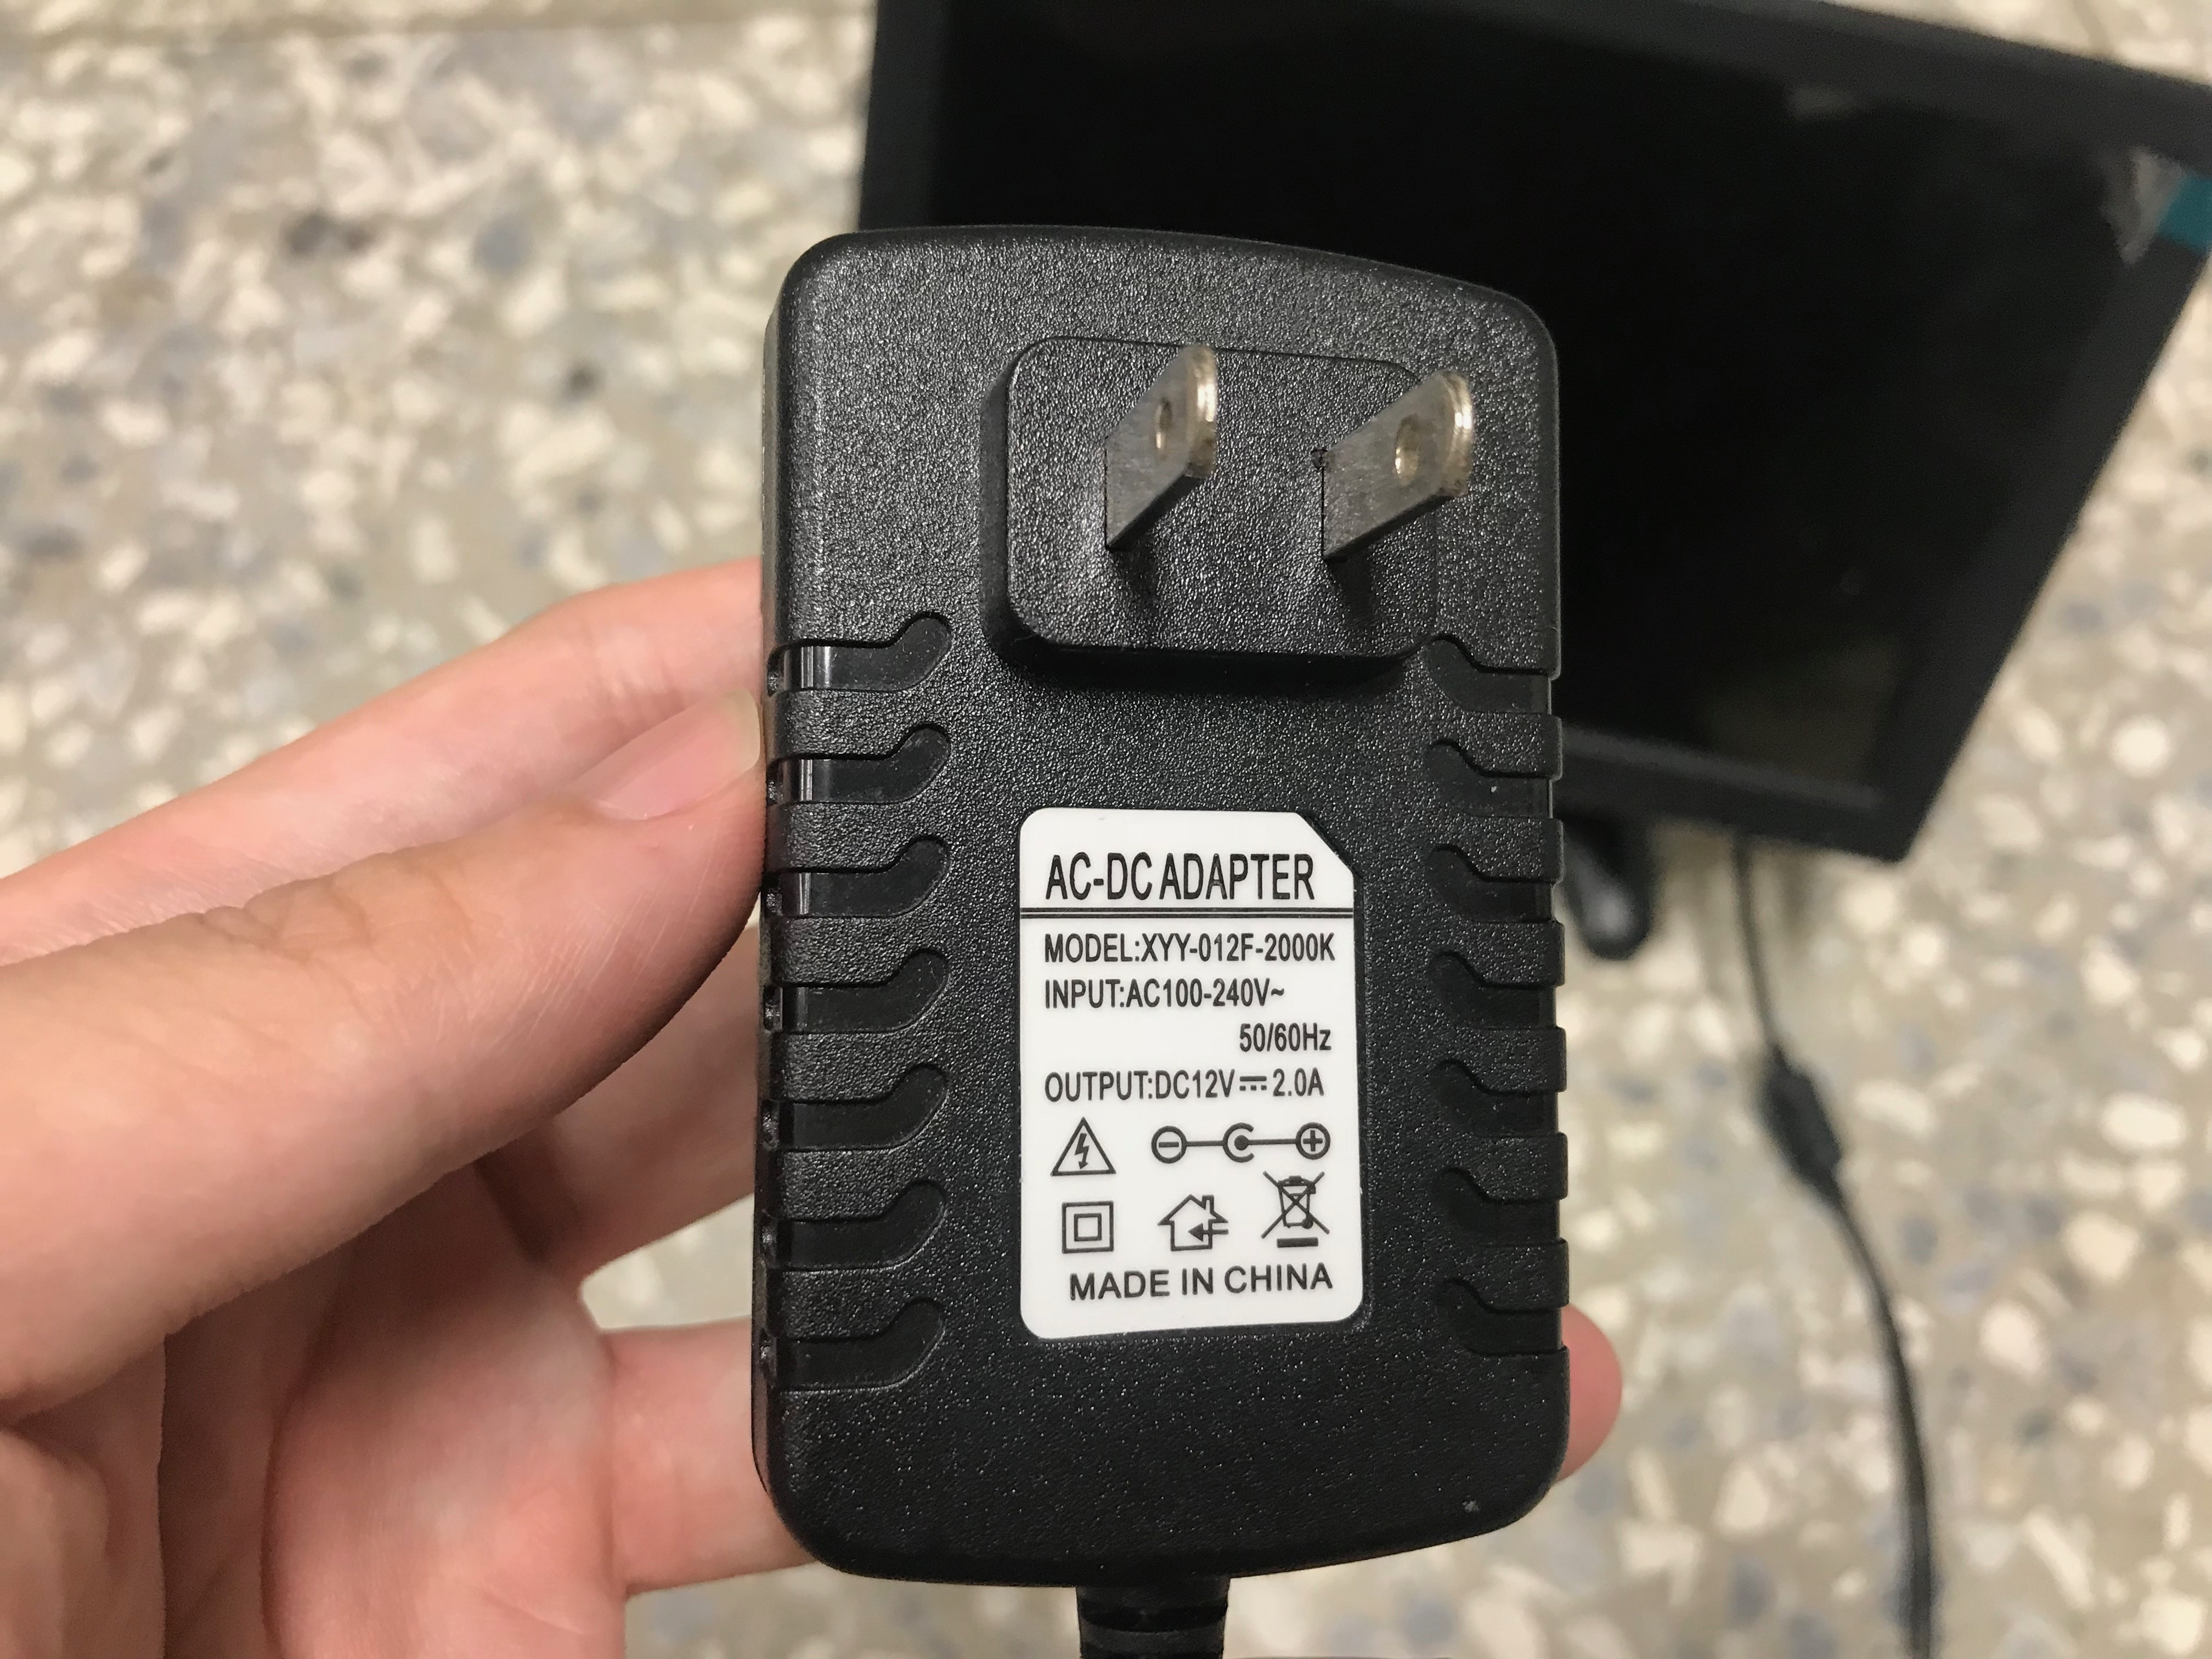
\includegraphics[width=0.6\textwidth]{img/8_spe_minimonitor_adapter}
  \caption{Mini-monitor adapter specifications}
\end{figure}
\begin{figure}[h]
  \centering
  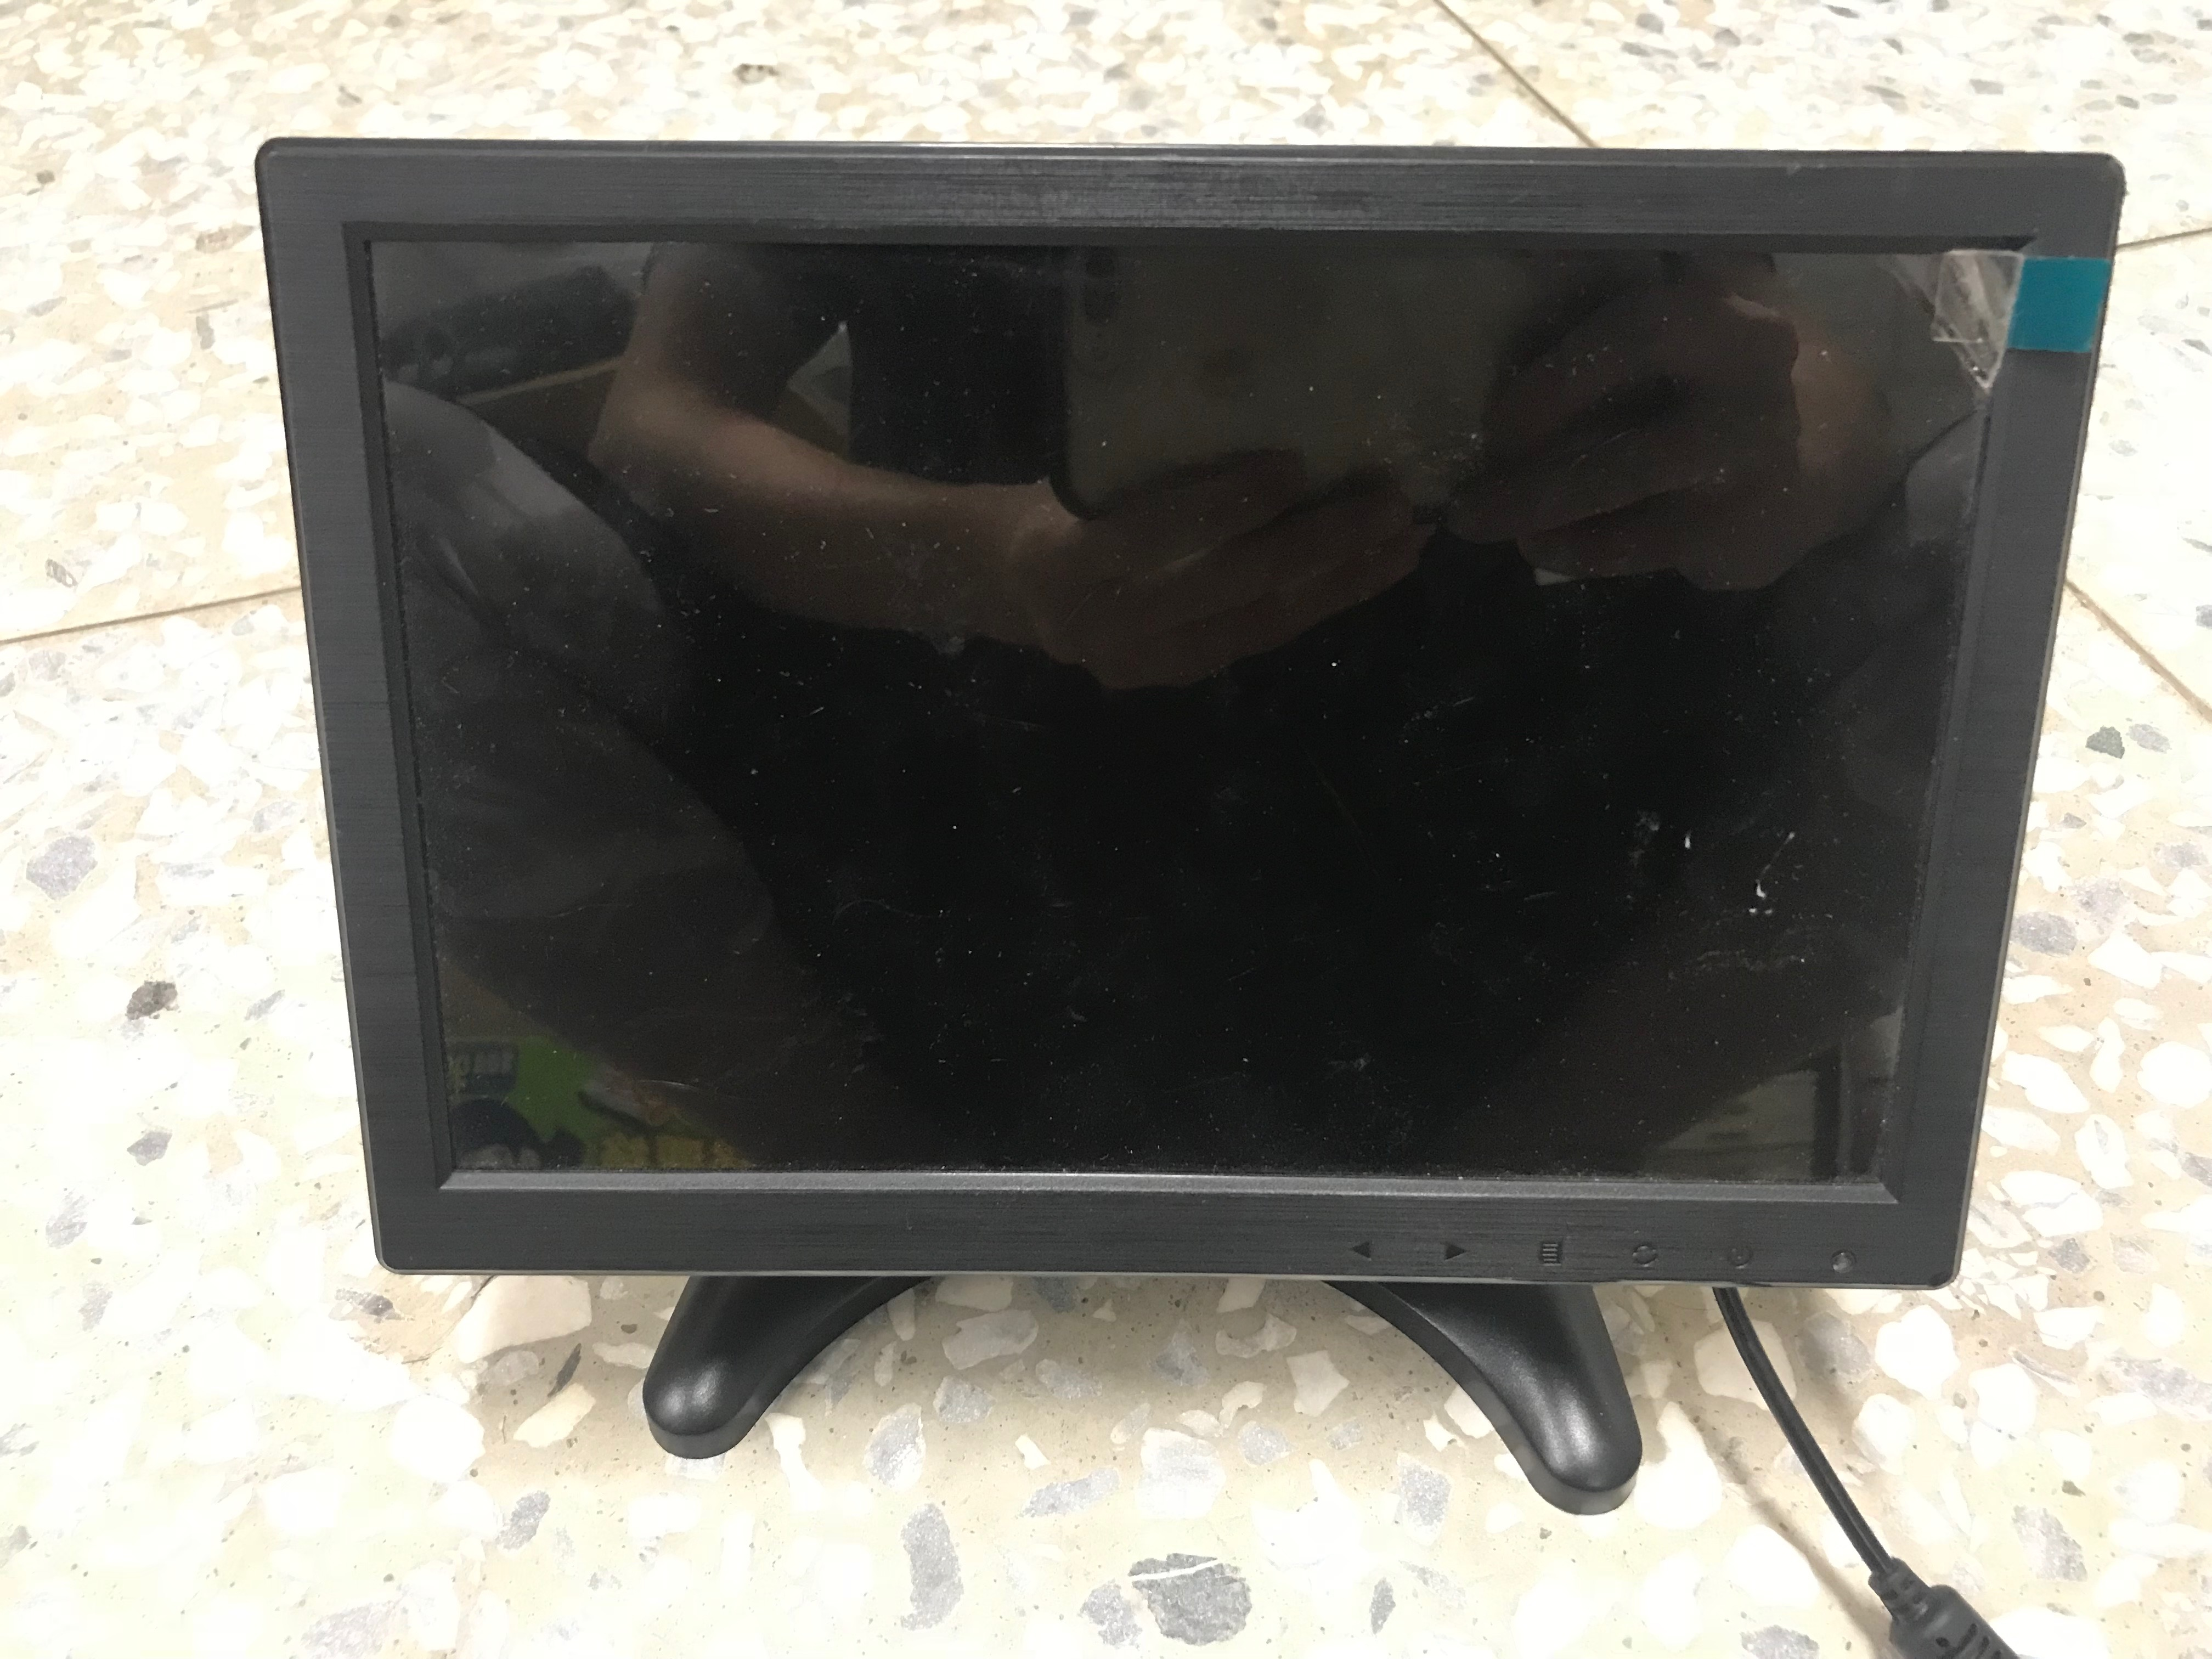
\includegraphics[width=0.6\textwidth]{img/8_pic_minimonitor}
  \caption{Mini-monitor}
\end{figure}

\clearpage

\subsection{Laptop}
\begin{figure}[h]
  \centering
  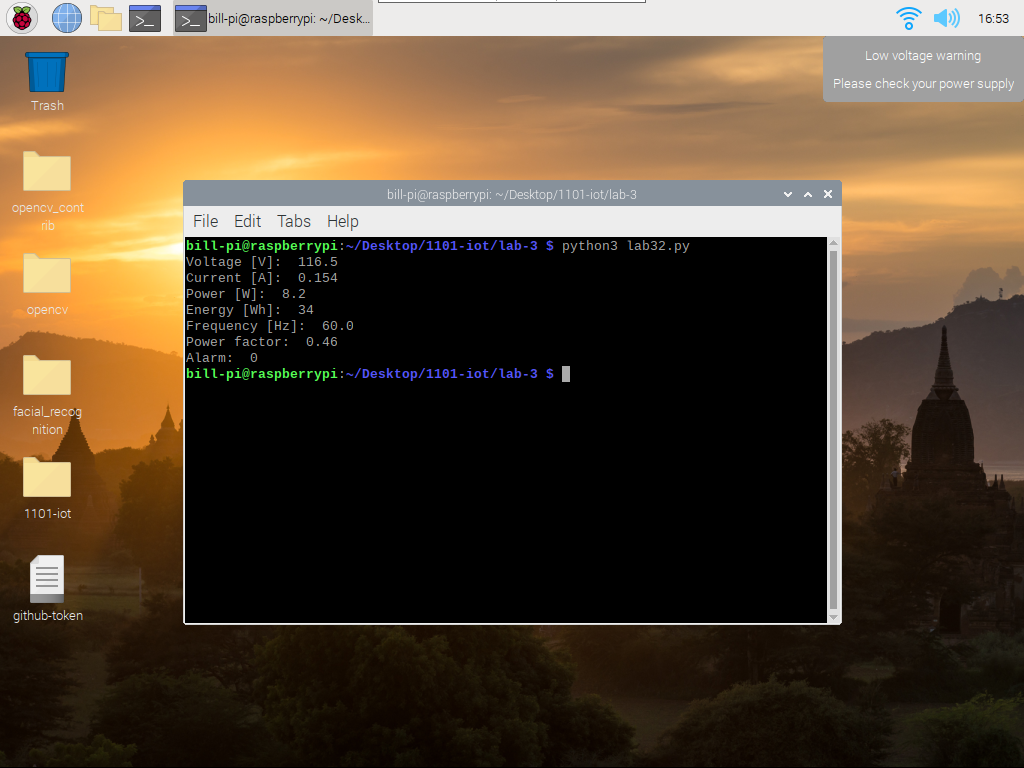
\includegraphics[width=0.6\textwidth]{img/9_res_laptop}
  \caption{Laptop result}
\end{figure}
\begin{figure}[h]
  \centering
  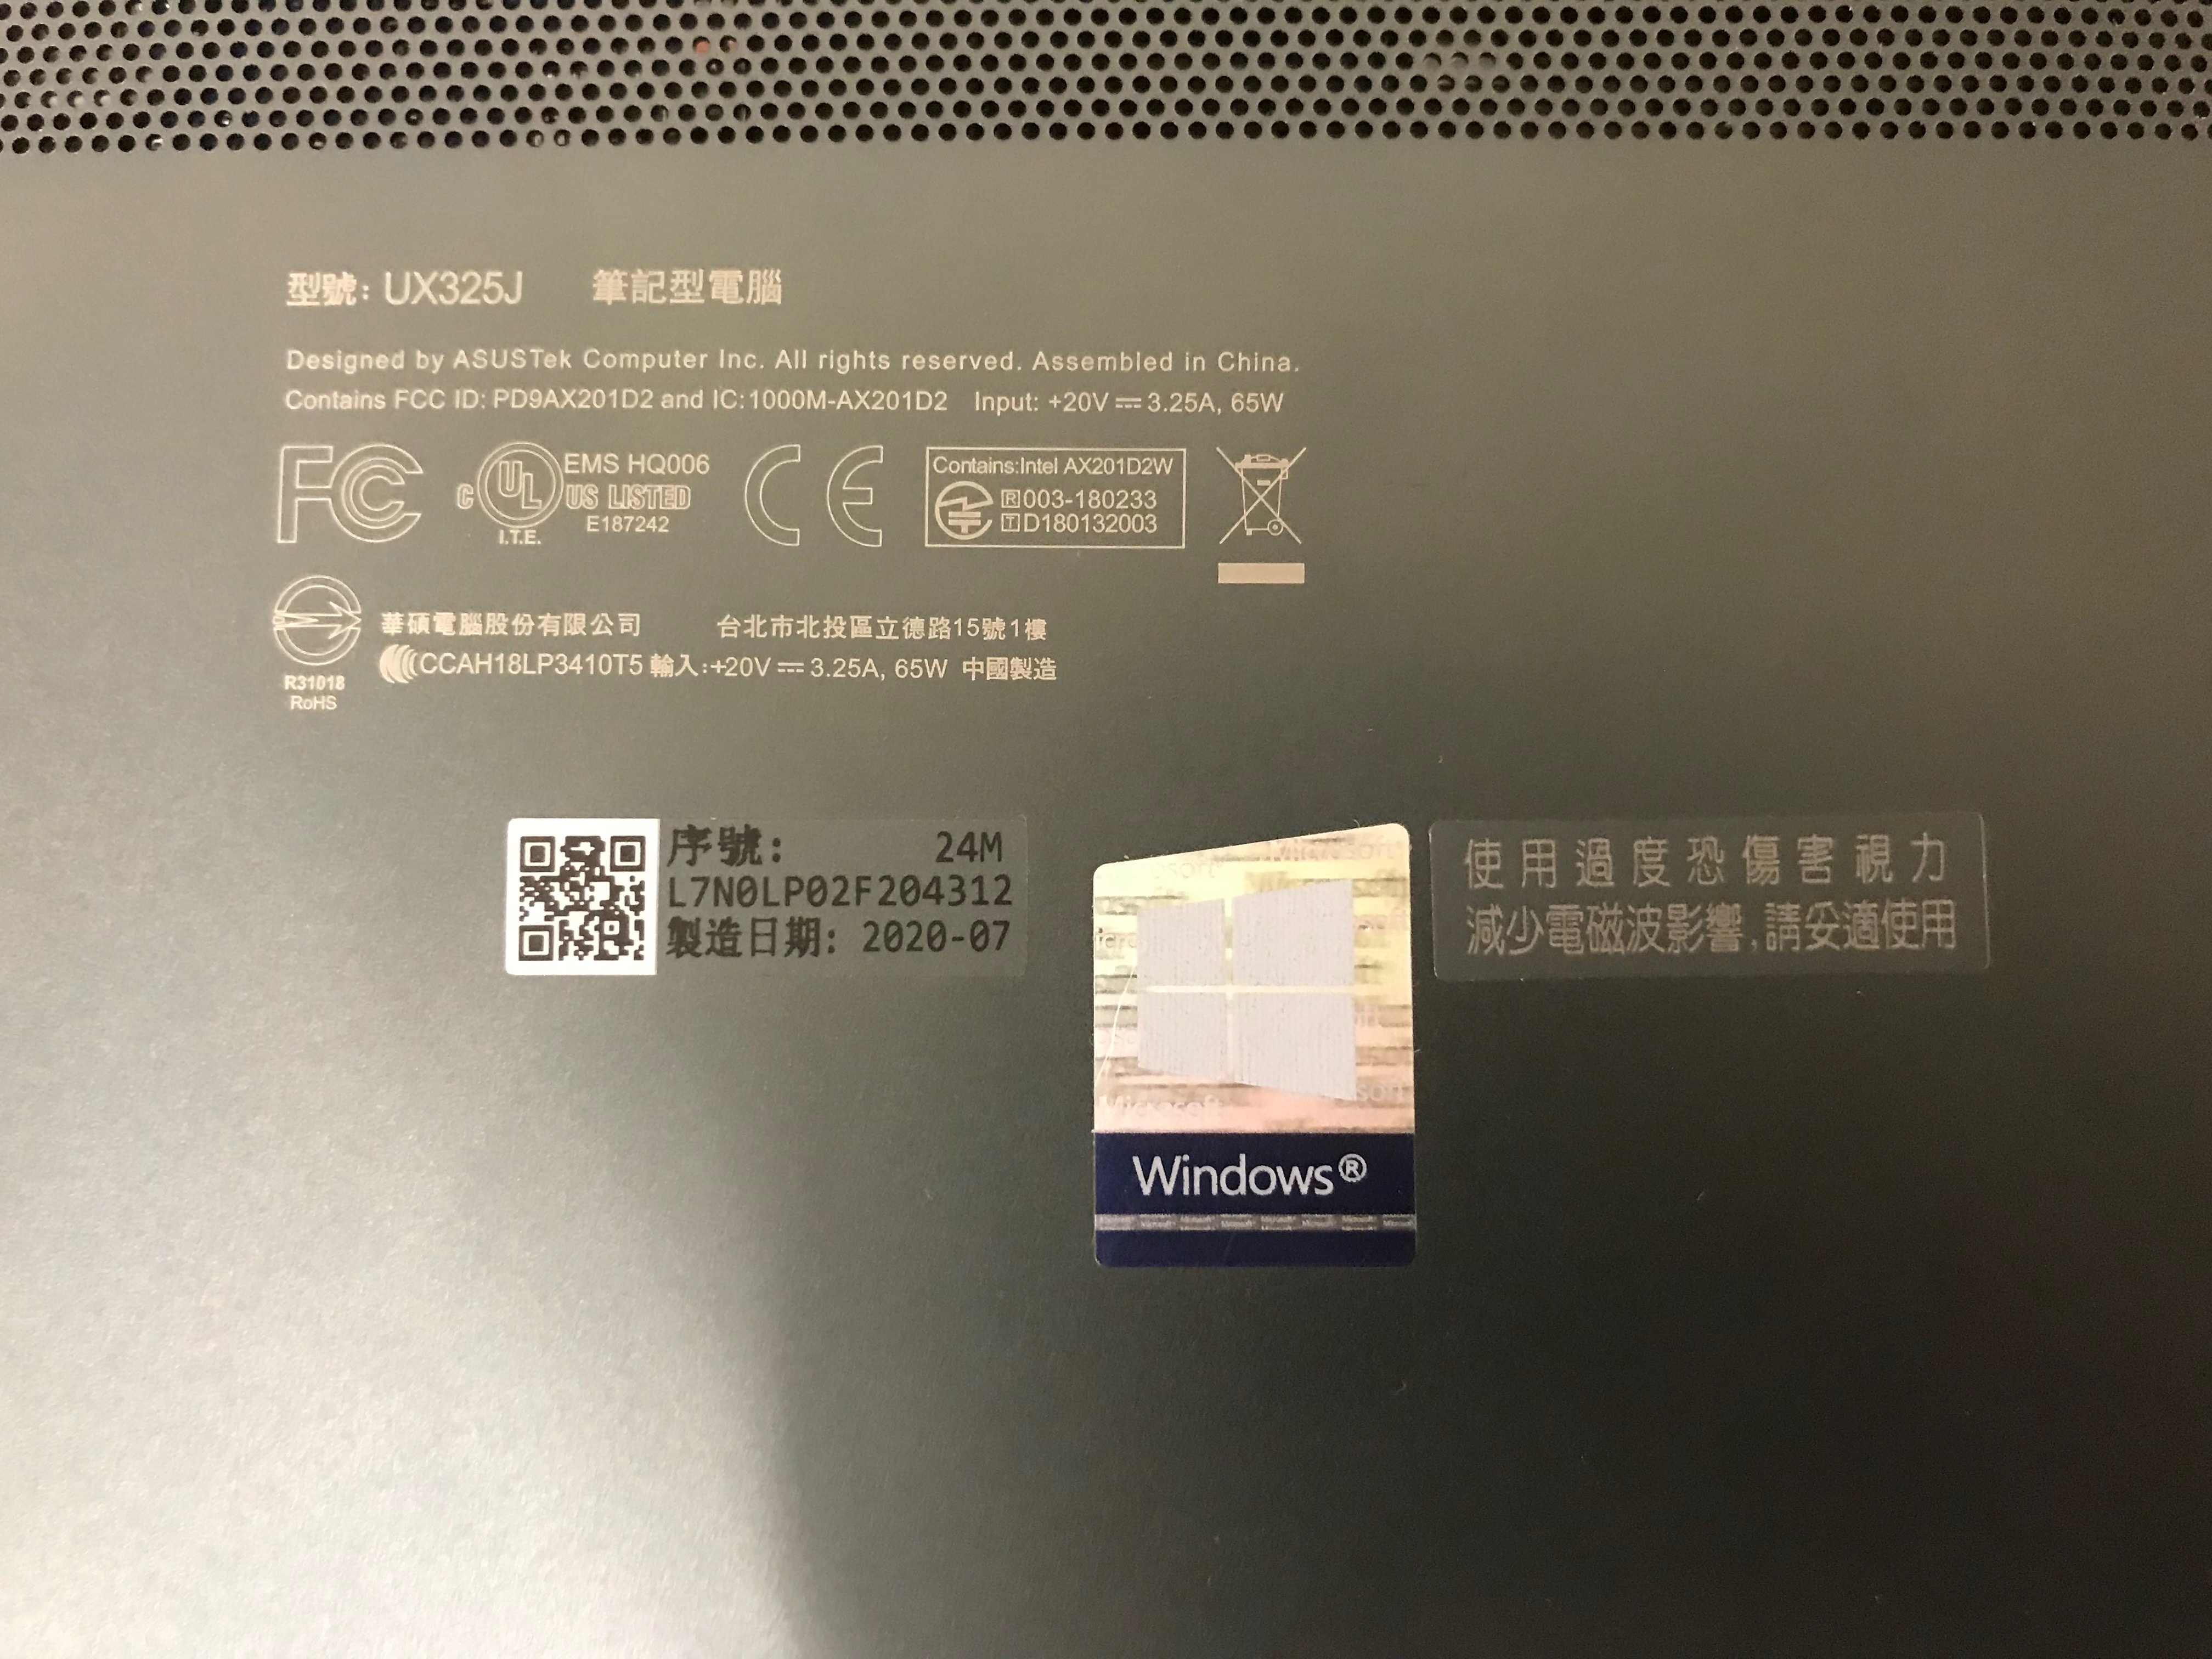
\includegraphics[width=0.6\textwidth]{img/9_spe_laptop}
  \caption{Laptop specifications}
\end{figure}
\begin{figure}[h]
  \centering
  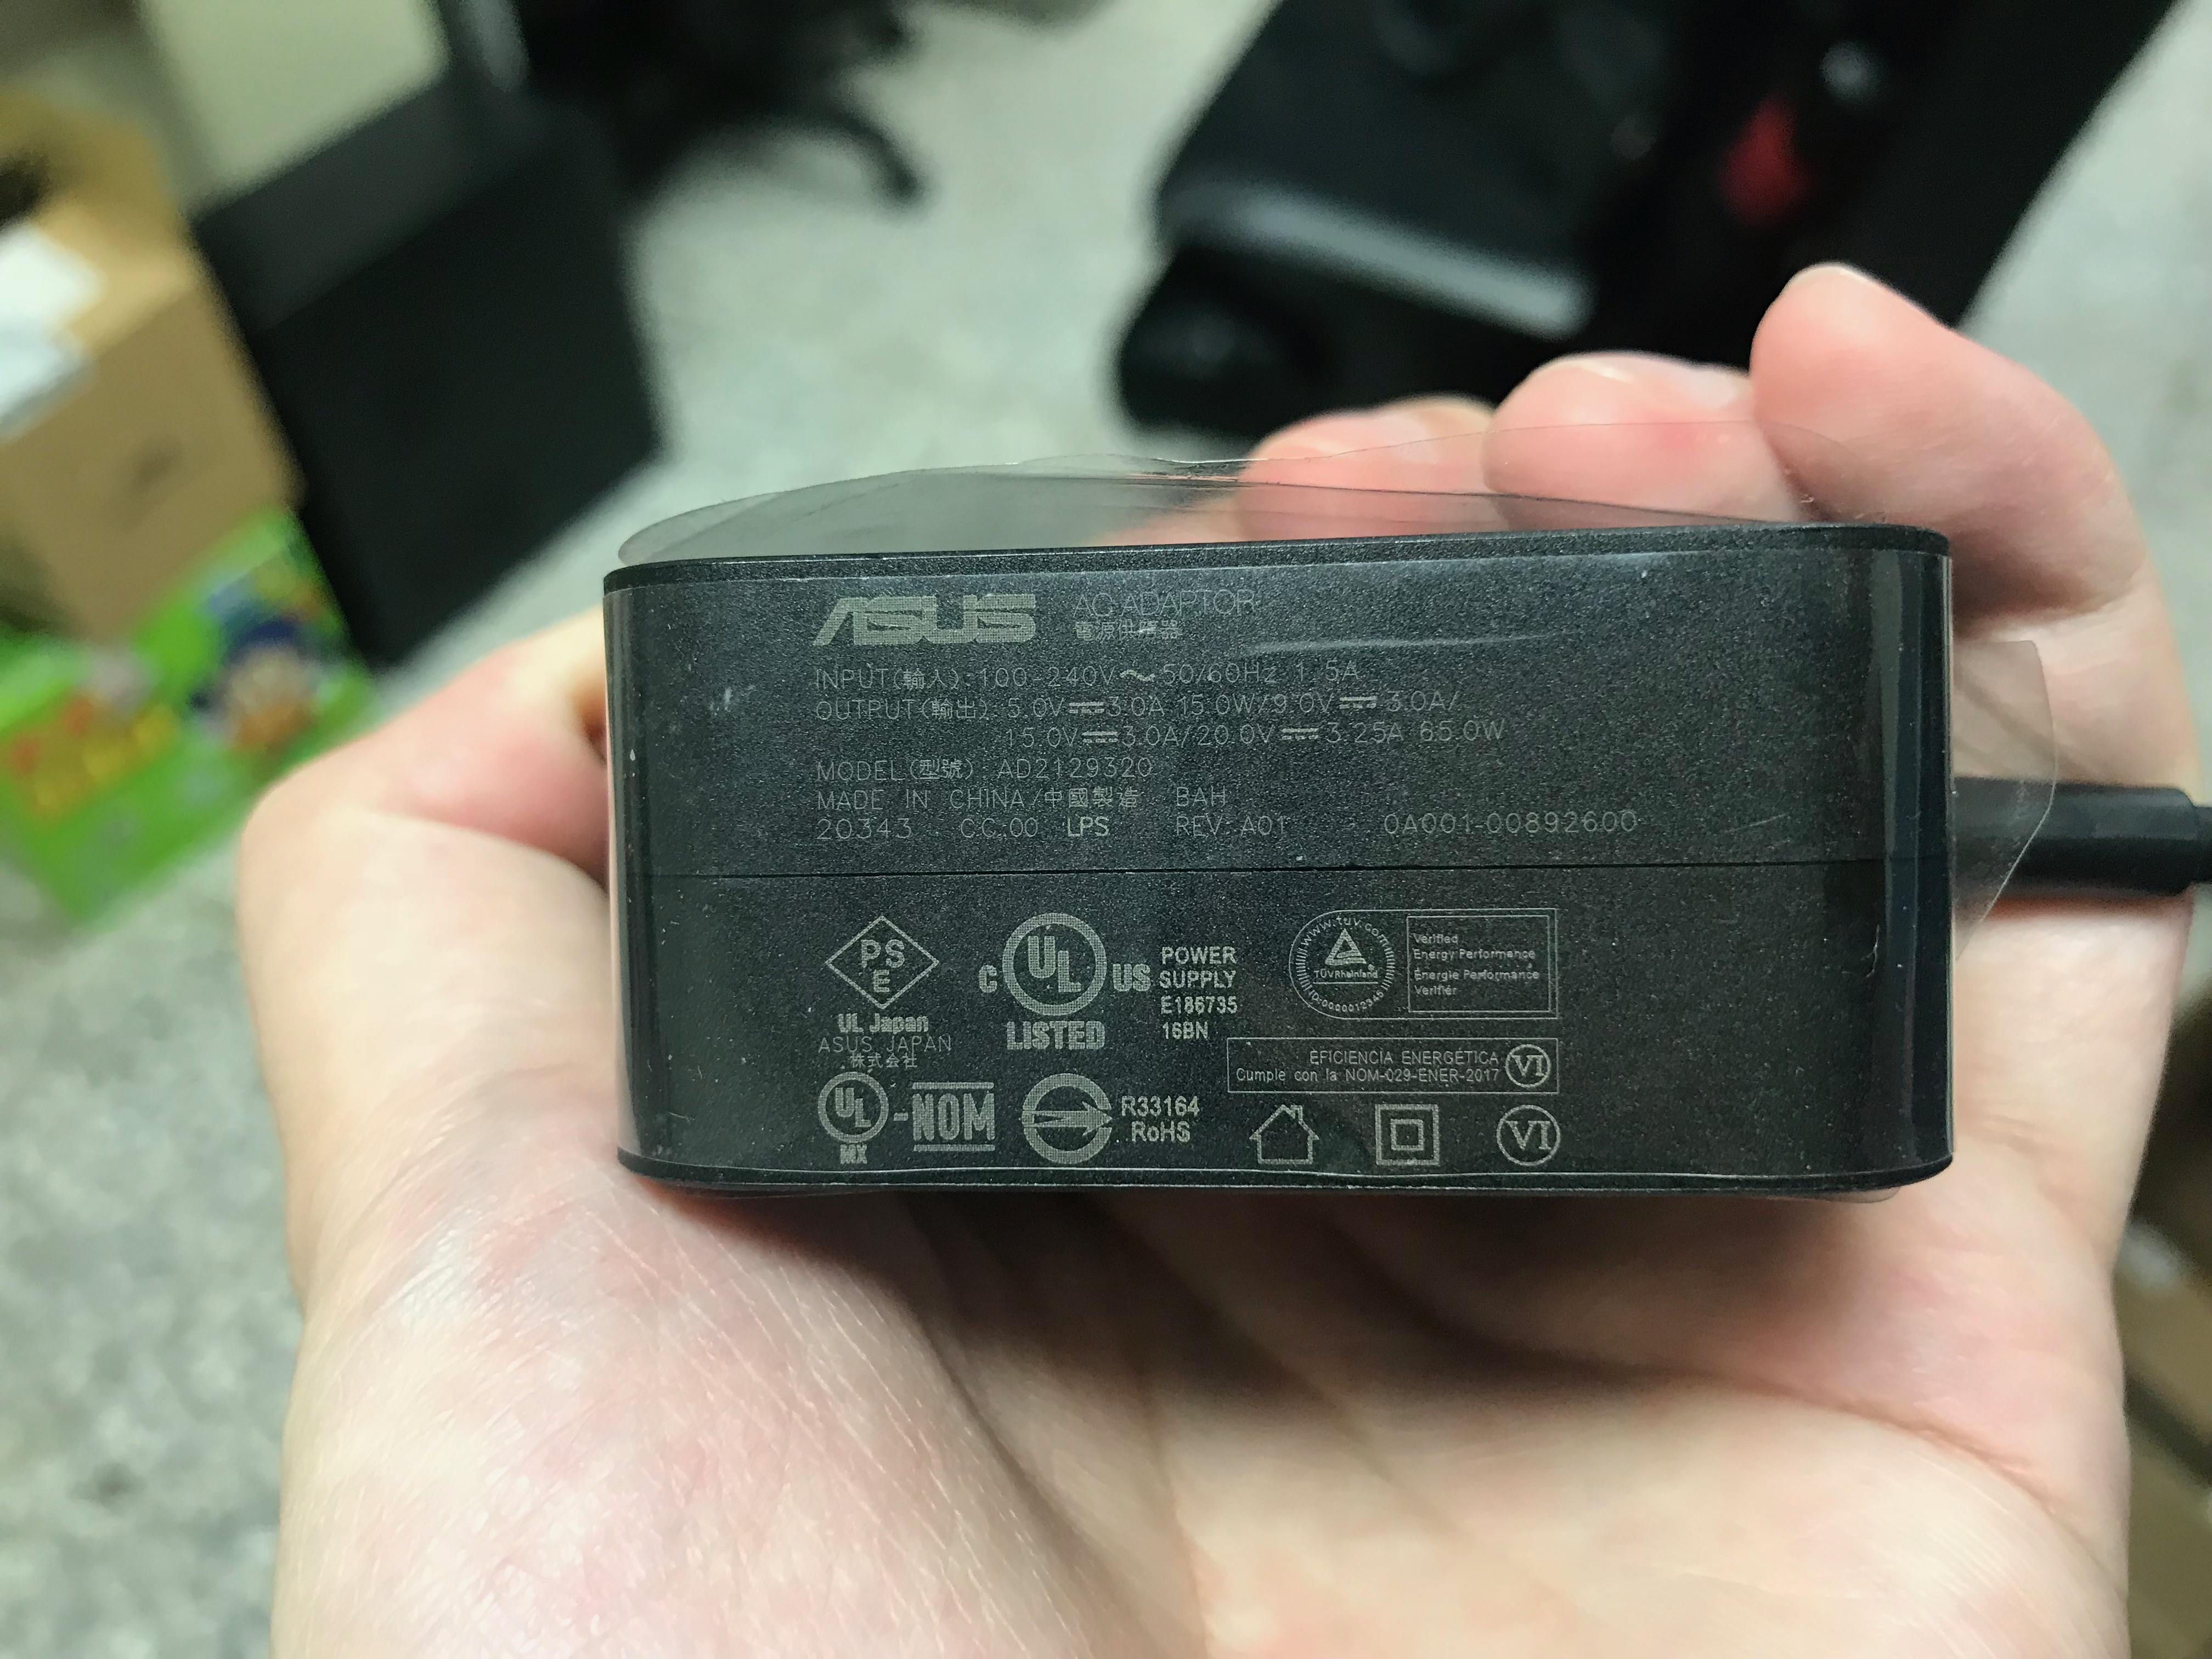
\includegraphics[width=0.6\textwidth]{img/9_spe_laptop_adapter}
  \caption{Laptop adapter specifications}
\end{figure}
\begin{figure}[h]
  \centering
  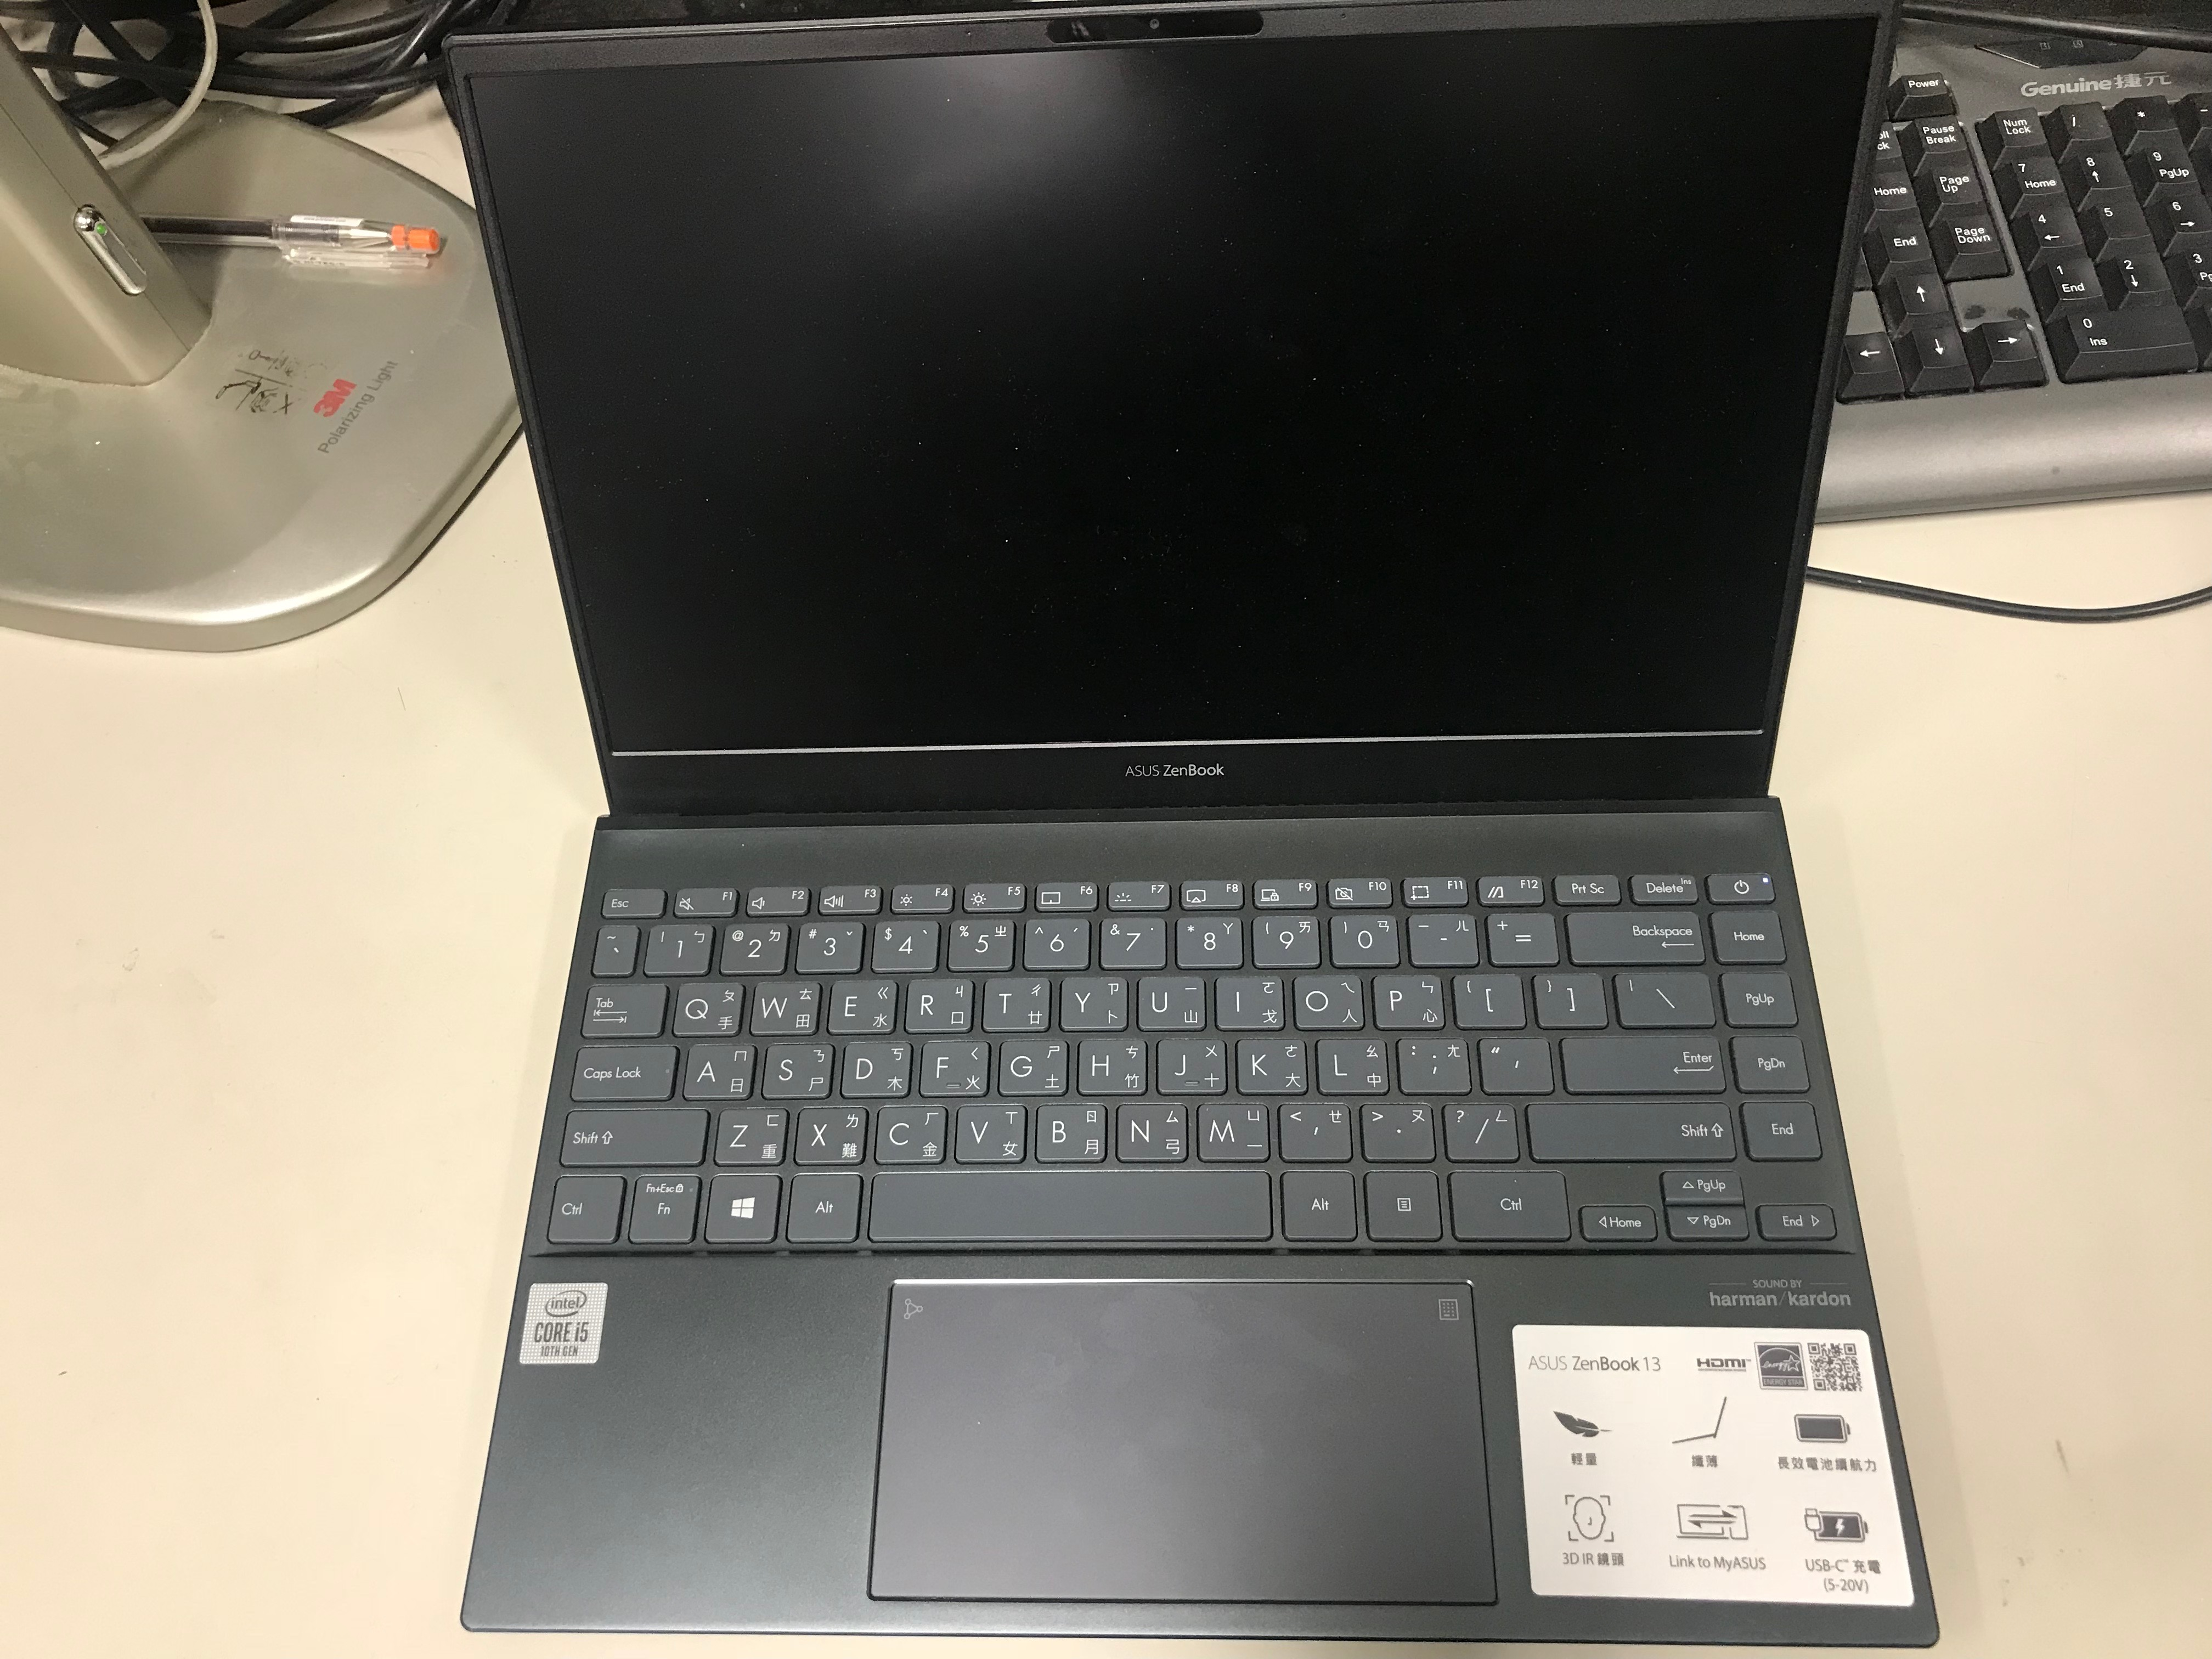
\includegraphics[width=0.6\textwidth]{img/9_pic_laptop}
  \caption{Laptop}
\end{figure}

\clearpage

\subsection{Phone}
\begin{figure}[h]
  \centering
  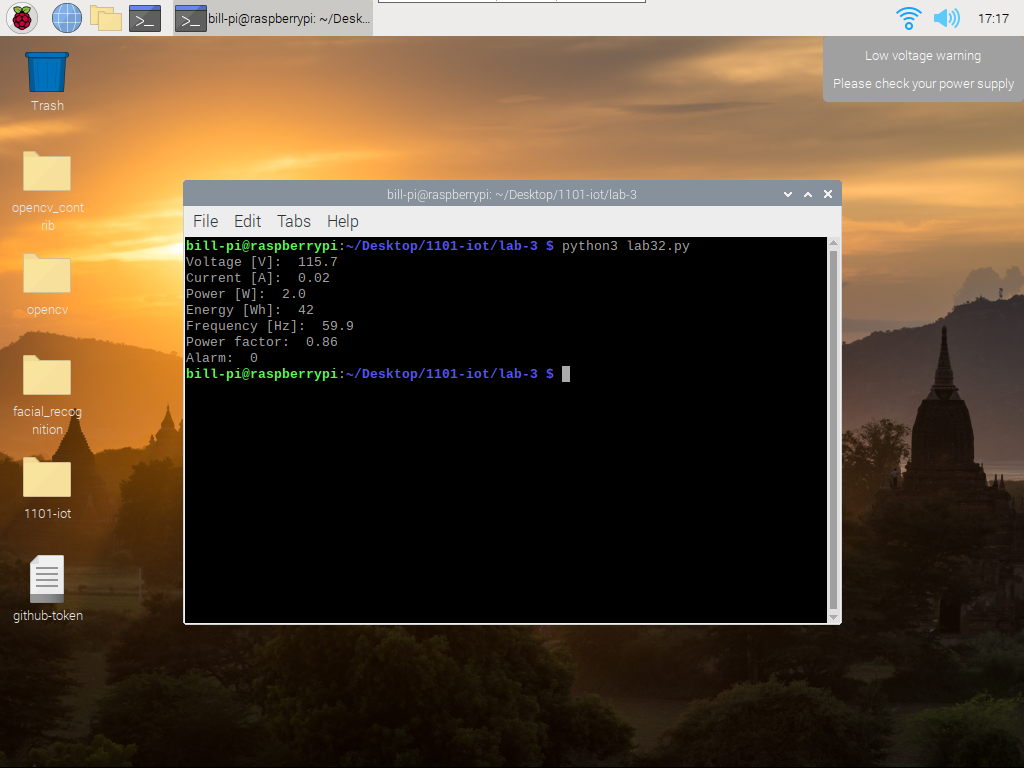
\includegraphics[width=0.6\textwidth]{img/10_res_phone}
  \caption{Phone result}
\end{figure}
\begin{figure}[h]
  \centering
  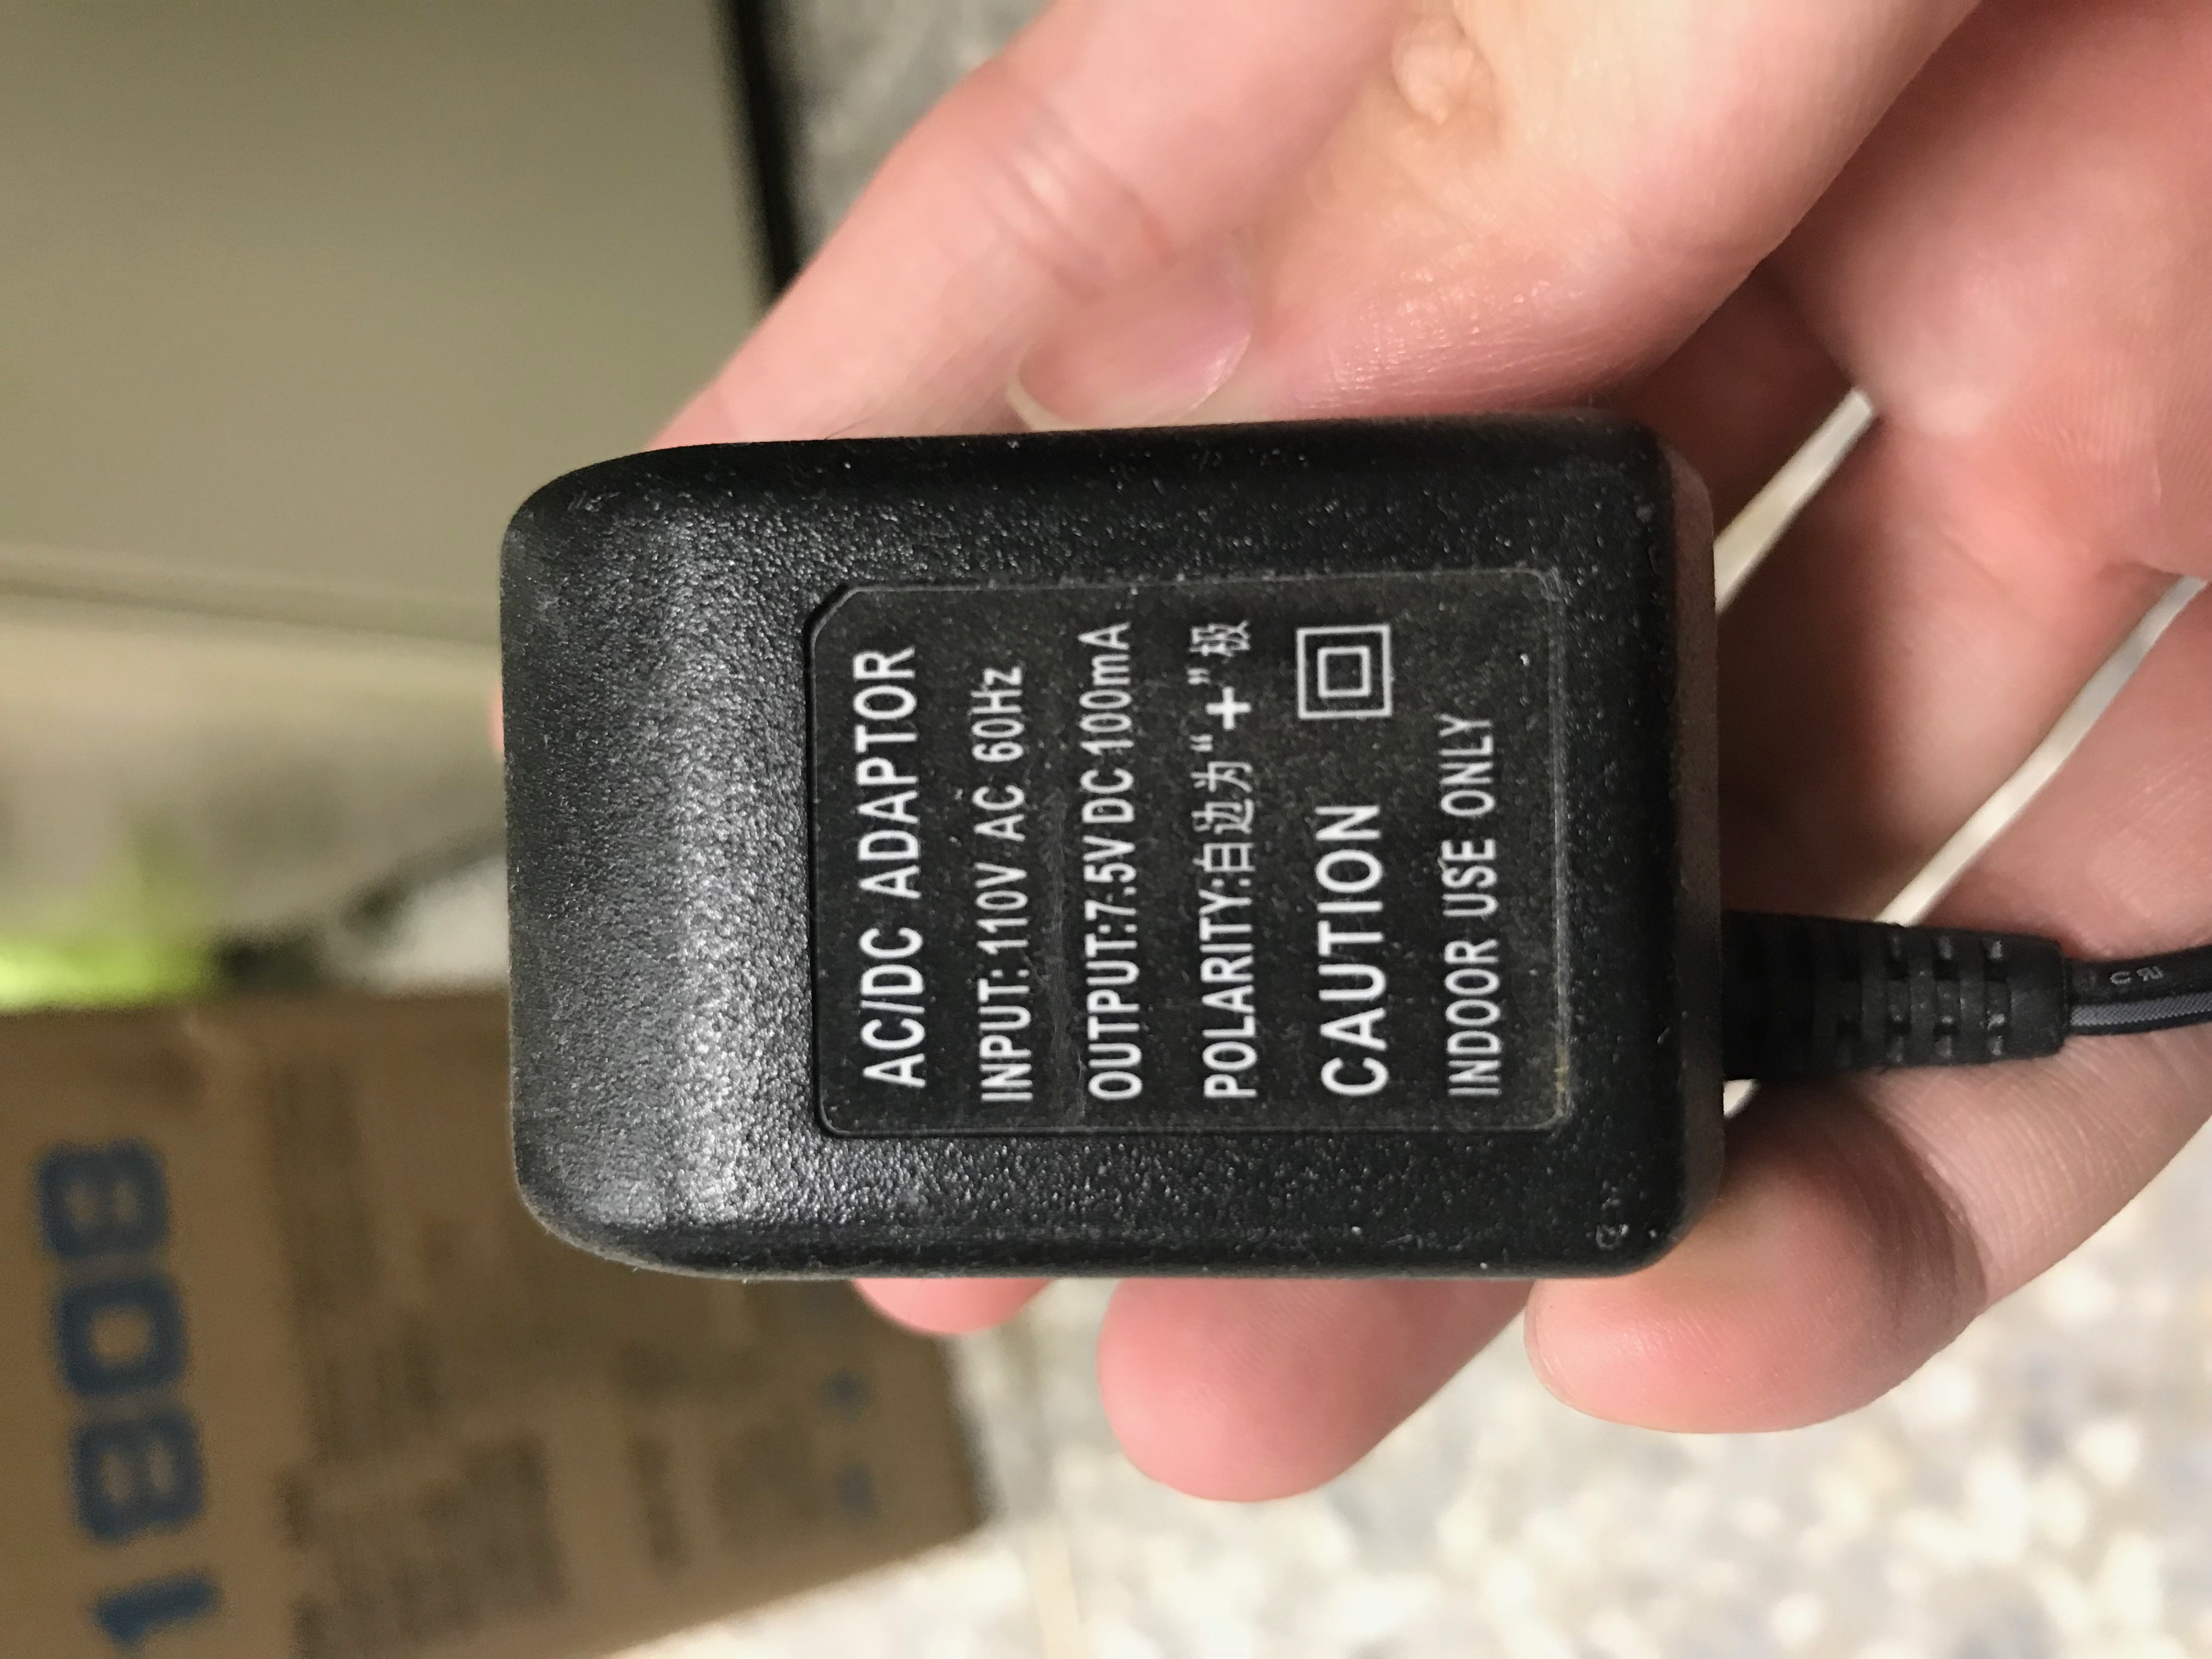
\includegraphics[angle=-90, origin=c, width=0.45\textwidth]{img/10_spe_phone_adapter}
  \caption{Phone adapter specifications}
\end{figure}
\begin{figure}[h]
  \centering
  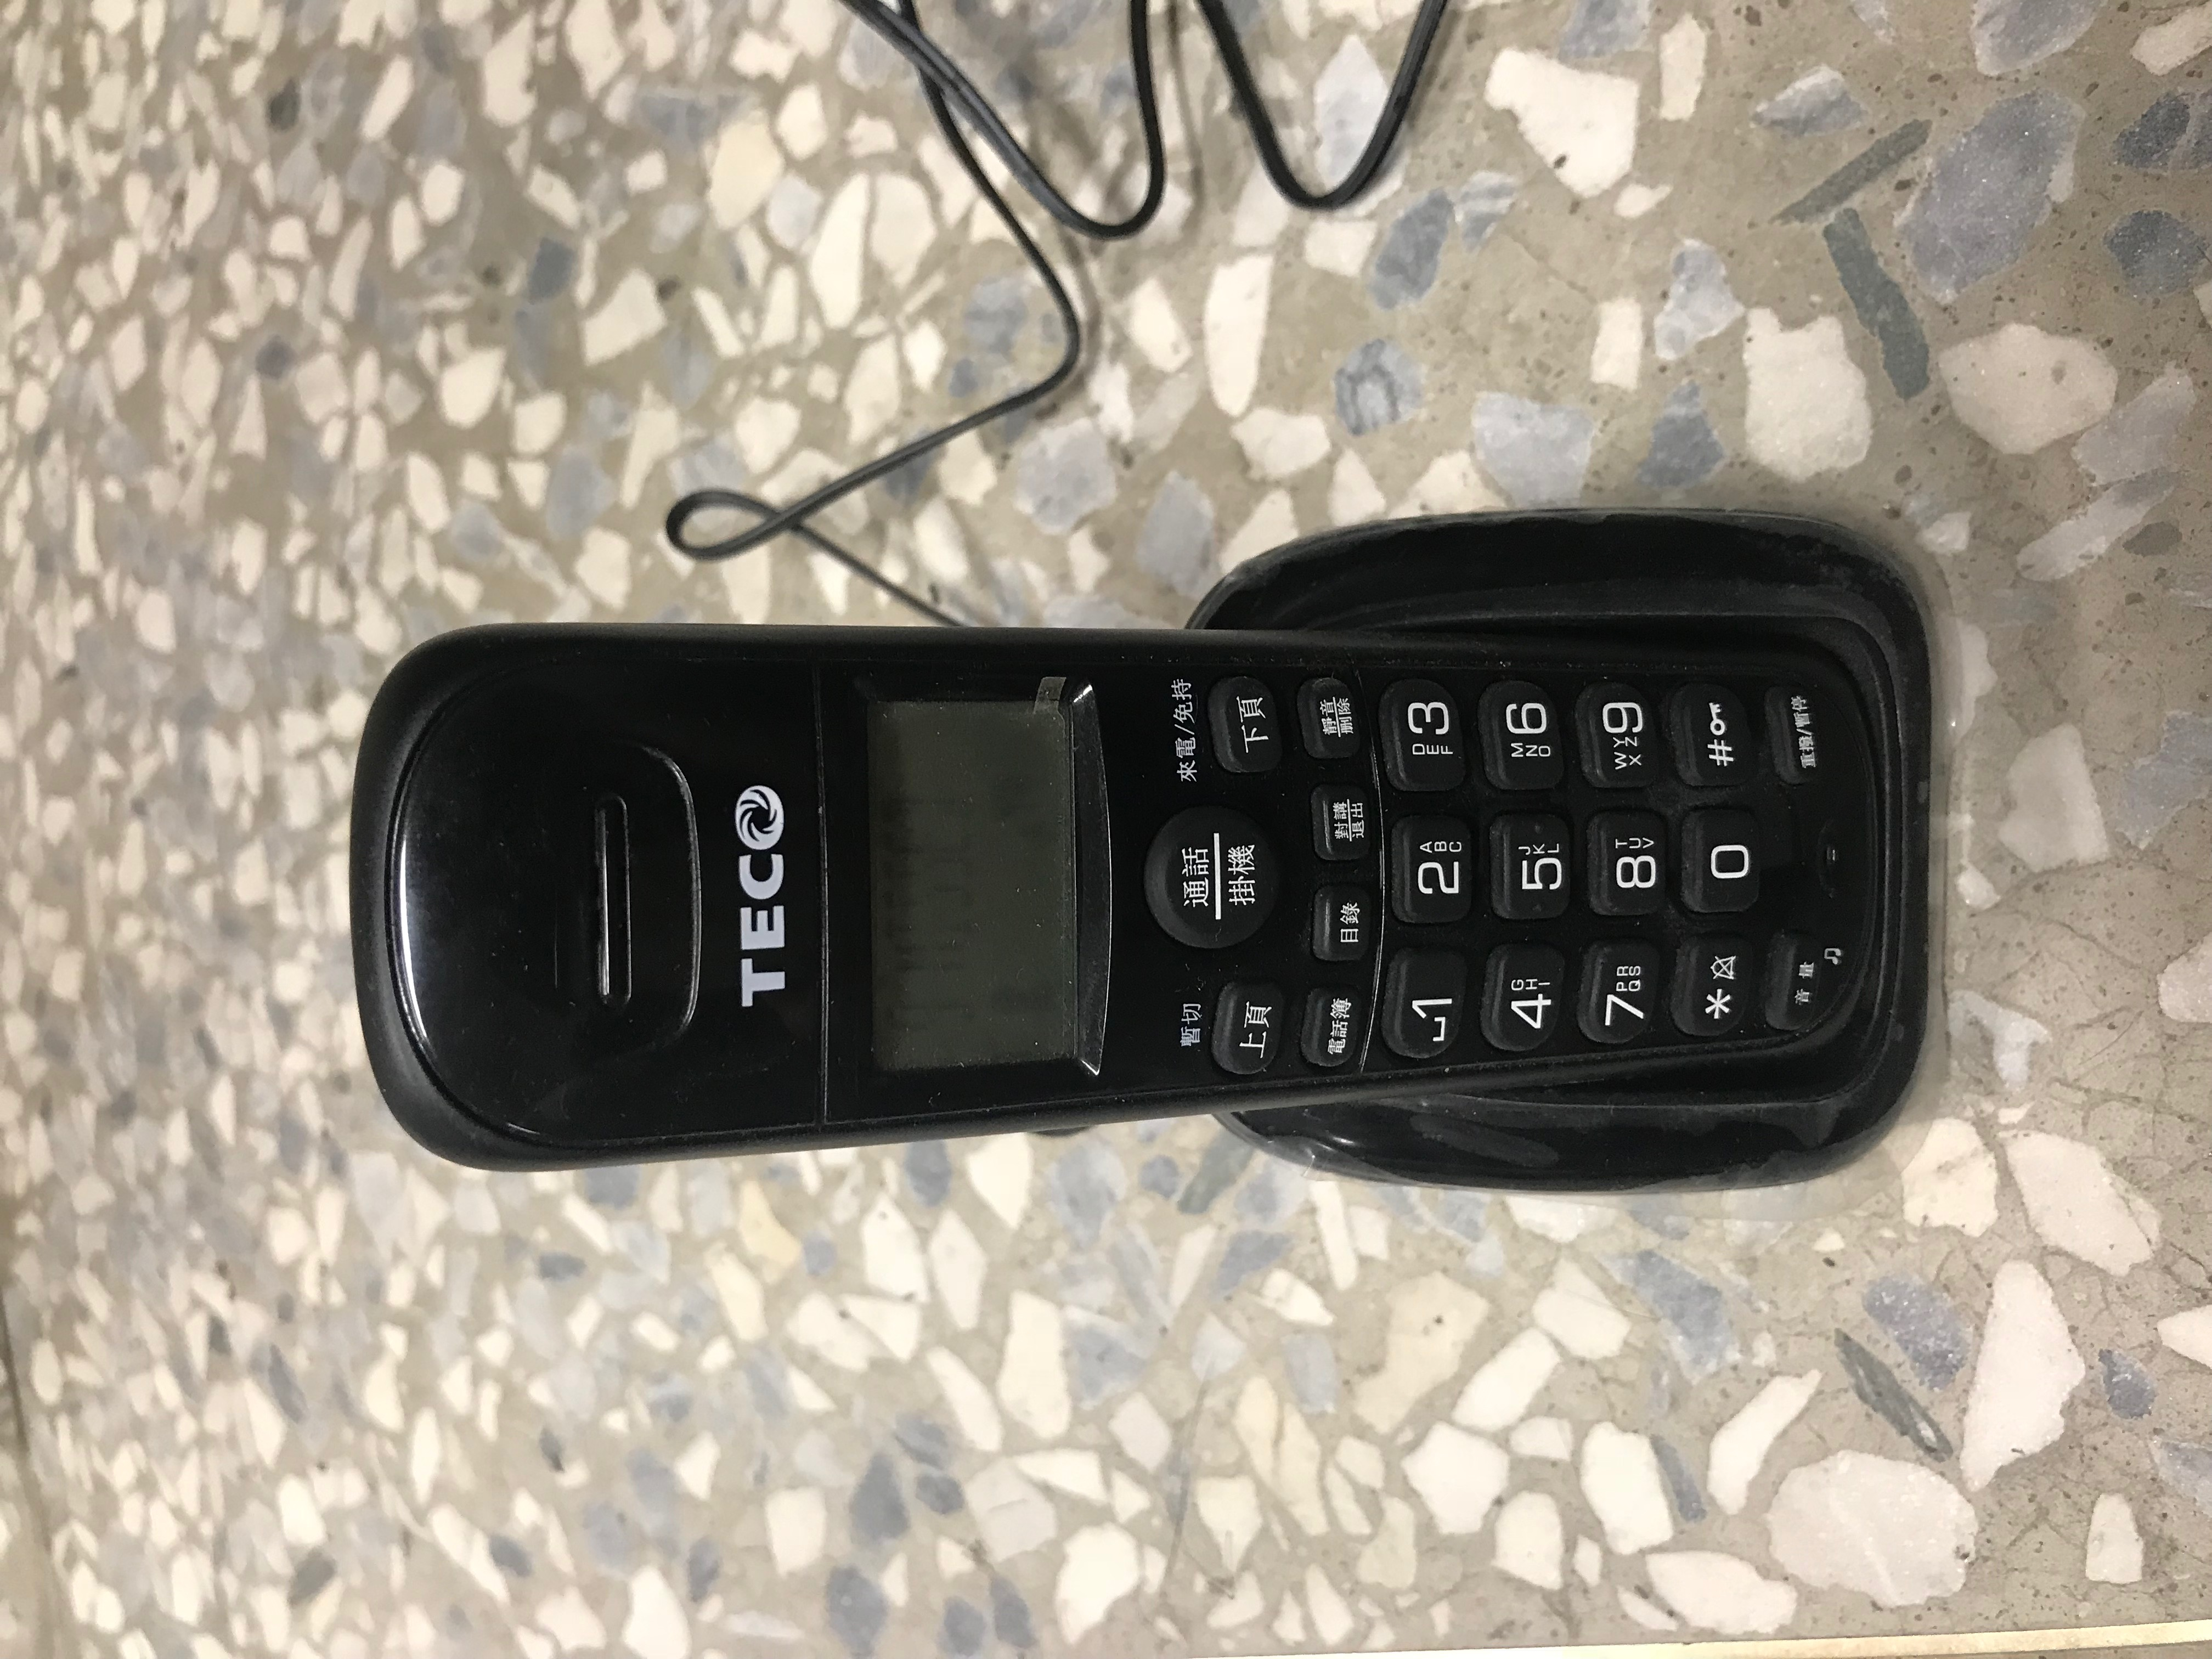
\includegraphics[angle=-90, origin=c, width=0.45\textwidth]{img/10_pic_phone}
  \caption{Phone}
\end{figure}

\end{document}
